\documentclass[a4paper,10pt]{article}
\usepackage{graphicx}
\usepackage{caption}
\usepackage{enumitem}
\usepackage{multicol}
\usepackage{mathtools}
\usepackage{amsmath,amsthm,amssymb,cancel,bm}
\usepackage{floatrow}
\setcounter{tocdepth}{2}
\usepackage{geometry}
\geometry{total={210mm,297mm},
left=25mm,right=25mm,%
bindingoffset=0mm, top=20mm,bottom=20mm}
\newcommand{\linia}{\rule{\linewidth}{0.5pt}}
\AtBeginDocument{%
   \setlength\abovedisplayskip{-3pt}
   \setlength\belowdisplayskip{5pt}}

\usepackage{hyperref}
\hypersetup{colorlinks=true,linkcolor=blue,citecolor=green,filecolor=cyan,urlcolor=magenta}

% my own titles
\makeatletter
\renewcommand{\maketitle}{
\begin{center}
\vspace{2ex}
{\huge \textsc{\@title}}
\vspace{1ex}
\\
\linia\\
\@author
\vspace{4ex}
\end{center}
}
\makeatother

% custom footers and headers
\usepackage{fancyhdr,lastpage}
\pagestyle{fancy}
\lhead{}
\chead{}
\rhead{}
\renewcommand{\headrulewidth}{0pt}
\lfoot{General Qualifying Exam Solutions}
\cfoot{}
\rfoot{Page \thepage\ /\ \pageref*{LastPage}}

% --------------------------------------------------------------
%
%                           TITLE PAGE
%
% --------------------------------------------------------------

\begin{document}
\hfill{\textit{Last modified \today}}
\title{General Qualifying Exam Solutions: Physics}
\author{Jessica Campbell, Dunlap Institute for Astronomy \& Astrophysics (UofT)}
\date{\today}
\maketitle

\tableofcontents



% --------------------------------------------------------------
%
%
%                              PHYSICS 
%
%
% --------------------------------------------------------------

\newpage
\section{Physics}

% --------------------------------------------------------------
%               1. 
% --------------------------------------------------------------

\subsection{Question 1}

Draw the geometry of gravitational microlensing of one star by another, and estimate the angular displacement of the background star's image.

\subsubsection{Short answer}

Answer.

\subsubsection{Additional context}

The first written account of the deflection of light by gravity appeared in the article ``On The Deflection Of Light Ray From Its Straight Motion Due To The Attraction Of A World Body Which It Passes Closely,'' by Johann Soldner in 1804. In his article Soldner predicted that a light ray passing close to the solar limb would be deflected by an angle  $\alpha=0.84\,{\rm arcsec}$. More than a century later,in 1919, Albert Einstein directly addressed
the influence of gravity on light. At this time Einstein's General Theory of Relativity was not fully developed. This is the reason why Einstein obtained (unaware of the earlier result) the same value for the deflection angle as Soldner had calculated with Newtonian physics. In this paper Einstein found $\alpha=2GM_\odot/c^2R_\odot=0.83\,{\rm arcsec}$ for the deflection angle of a light ray grazing the Sun (here $M_\odot$ and $R_\odot$ are the mass and radius of the Sun, $c$ and $G$ are the speed of light and the gravitational constant respectively). 

{\noindent}Einstein emphasized his wish that astronomers investigate this equation. In 1913 Einstein contacted the director of Mount Wilson observatory, George Hale, and asked if it will be possible to measure the positions of stars near the Sun during the day in order to establish the angular deflection effect of the Sun. The first observational attempt to test Einstein's prediction for the deflection angle was in 1914. This attempt was never accomplished which was fortunate for Einstein whose predicted value for the angular deflection was actually wrong. With the completion of the General Theory of Relativity in 1916, Einstein was the first to derive the correct formula for the deflection angle $\alpha$ of a light passing at a distance $r$ from an object with mass $M$ as

\begin{align*}
    \alpha = \frac{4GM}{c^2}\frac{1}{r^2} ~ [{\rm arcsec}].
\end{align*}

{\noindent}The additional factor of two (compared to the ``Newtonian'' value) is due to the spatial curvature which is missed if photons are just treated as particles.

{\noindent}For the Sun, Einstein obtained

\begin{align*}
    \alpha_\odot = \frac{4GM_\odot}{c^2}\frac{1}{R_\odot^2} = 1.74 ~ [{\rm arcsec}].
\end{align*}

{\noindent}This value was first confirmed to within $20\%$ by Arthur Eddington and his group during a Solar total eclipse in 1919. Recently this value was confirmed to within $0.02\%$.

{\noindent}In 1924 Chwolson mentioned the idea of a ``factious double star.'' He also mentioned the symmetric case of one star exactly behind another star, resulting in a circular image. In 1936 Einstein also reported about the appearance of a ``luminous'' circle of perfect alignment between the source and the lens, such a configuration is called \textbf{Einstein Ring}. In 1937 Fritz Zwicky pointed out that galaxies are more likely to be gravitationally lensed than a star and that one can use the gravitational lens as natural telescope.

{\noindent}\textbf{The geometry of gravitational lensing}: Gravitational lensing results when light follows the straightest possible worldline (ie., a \textbf{geodesic}) as it travels though the curved spacetime around a massive object. It is analogous to the normal refraction of light by a glass lens that occurs as the light crosses the lens surface, passing from one index of refraction $n$ to another, where $n\equiv c/v$ is just the ratio of the speed of light in a vacuum to its speed $v$ in the medium. 

{\noindent}The apparent speed of light, the rate at which the spatial coordinates of a photon change, is called the \textbf{coordinate speed of light}. Starting with the Schwarzschild metric with ${\rm d}s=0$,

\begin{align*}
    0 = \left(c{\rm d}t \sqrt{1-\frac{2GM}{rc^2}}\right)^2 - \left(\frac{{\rm d}r}{\sqrt{1-\frac{2GM}{rc^2}}}\right)^2 - (r{\rm d}\theta)^2 - (2\sin\theta{\rm d}\alpha)^2,
\end{align*}

{\noindent}we can calculate the coordinate speed of a vertically travelling photon. Inserting ${\rm d}\theta={\rm d}\alpha=0$ shows that, in general, the coordinate speed of light in the radial direction is

\begin{align*}
    \frac{{\rm d}r}{{\rm d}t} = c\left(1-\frac{2GM}{rc^2}\right) = c\left(1-\frac{r_S}{r}\right) ~ [{\rm m\,s^{-1}}],
\end{align*}

{\noindent}When $r\gg r_S$, ${\rm d}r/{\rm d}t\simeq c$, as expected in flat spacetime. However, at $r=r_S$, ${\rm d}r/{\rm d}t=0$.

{\noindent}Thus, the effective ``index of refraction'' is

\begin{align*}
    n = \frac{c}{{\rm d}r/{\rm d}t} = \left(1-\frac{2GM}{rc^2}\right)^{-1} \simeq 1+ \frac{2GM}{rc^2} ~ [{\rm dimensionless}]
\end{align*}

{\noindent}for radially travelling light, assuming that $r_S/r\ll1$. At a distance of $10^4\,{\rm pc}$ from a galaxy with a mass of $10^11\,{\rm M_\odot}$, the effective index of refraction is $n=1+9.6\times10^{-7}$. (Of course, the light passing by the point mass will never be travelling exactly radially. This was merely used to estimate the magnitude of the effect of gravity in a gravitational lens.) Obviously, the deviation of the light from a straight line will be extremely small. 

\begin{figure}[t]
    \centering
    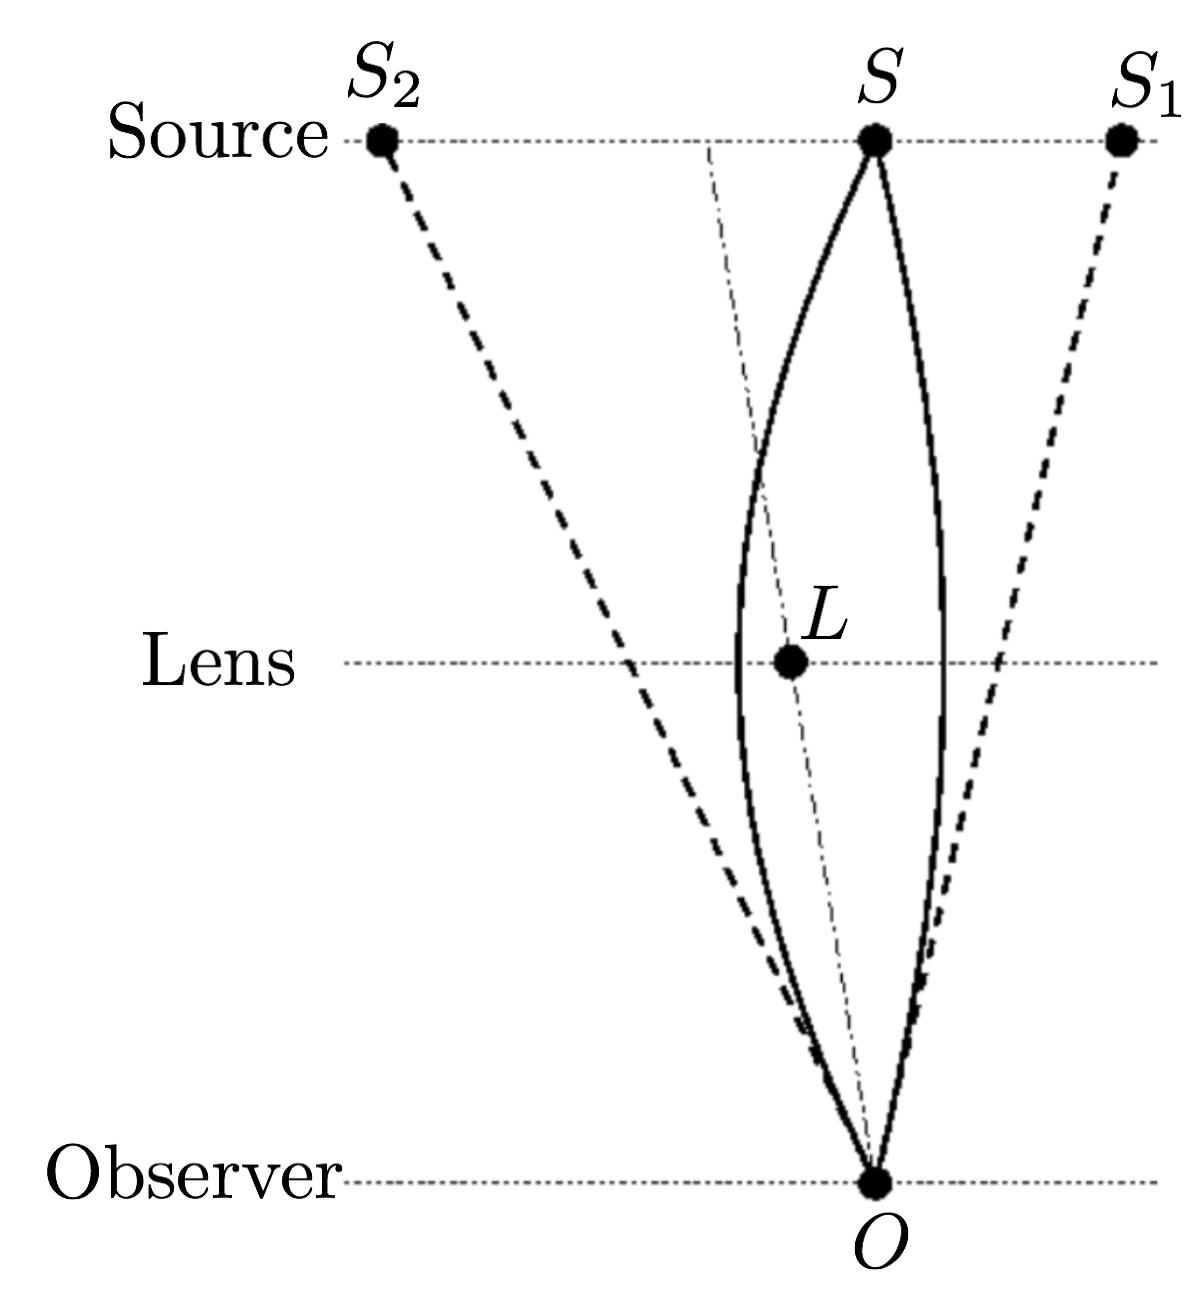
\includegraphics[width=7.5cm]{figures/GravitationalLens.png}
    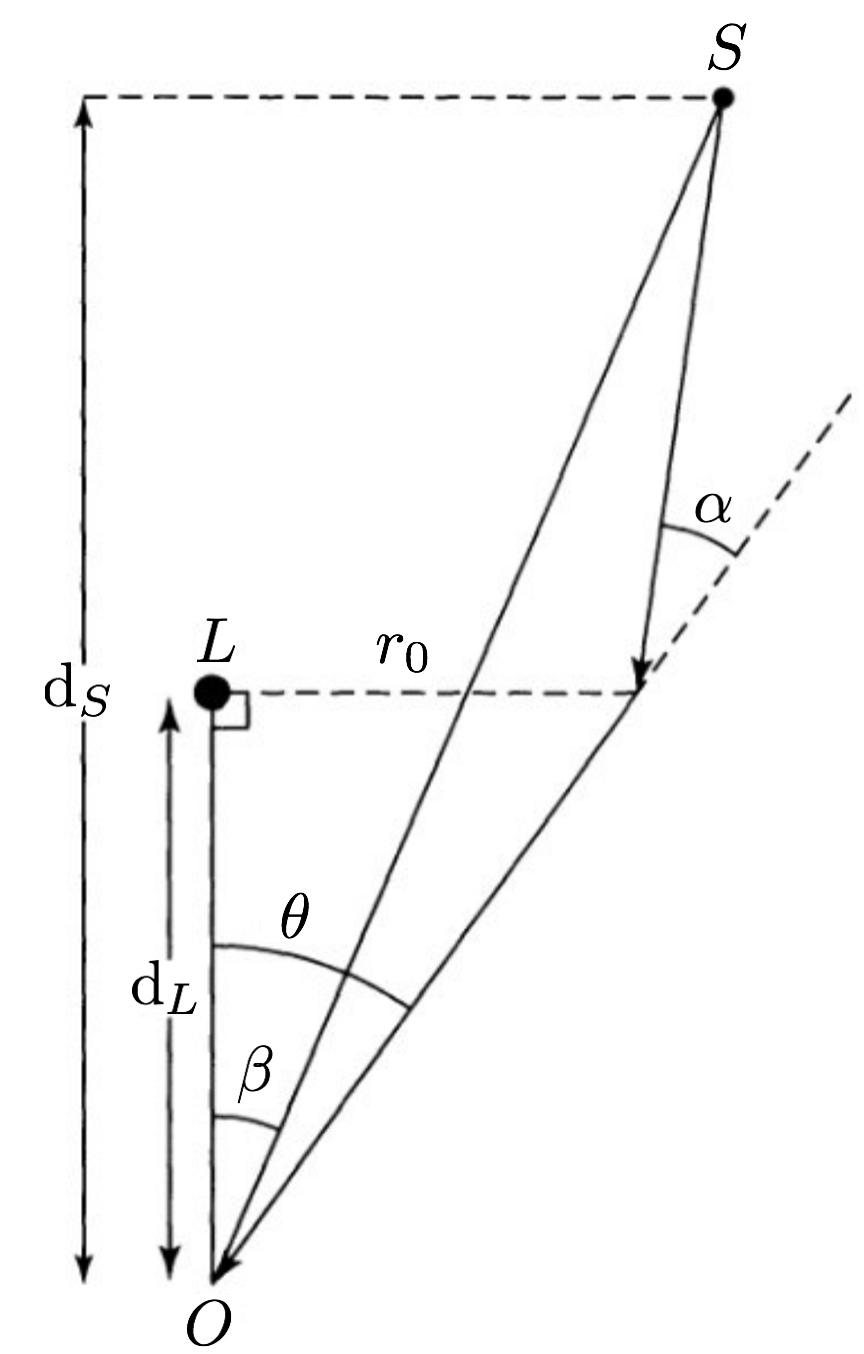
\includegraphics[width=5.5cm]{figures/GravitationalLensAngles.png}
    \caption{\footnotesize{\textbf{(Left)}: Setup of a gravitational lens. Figure taken from Abdo. \textbf{(Right)}: The geometry for a gravitational lens. The path of light is taken from a source at point $S$, as it is deflected through an angle $\alpha$, by the gravitational lens due to a point mass $M$ at point $L$. Figure taken from Carroll \& Ostlie (2007).}}
    \label{fig:gravitationallens}
\end{figure}

{\noindent}Figure \ref{fig:gravitationallens} shows the setup of a gravitational lens (left) as well as its detailed geometry (right). The path of light is taken from a source at point $S$, as it is deflected through an angle $\alpha$, by the gravitational lens due to a point mass $M$ at point $L$.

{\noindent}The angular deviation of a photon passing a distance $r_0$ (very nearly the distance of closest approach) from a mass $M$ is

\begin{align*}
    \alpha = \frac{4GM}{r_0c^2} ~ [{\rm rad}].
\end{align*}

{\noindent}which includes the factor of $2$ as a correction from the ``Newtonian'' value. The distance to the source is $d_S/\cos\beta\simeq d_S$ where $\beta\ll1$, and $d_L$ is the distance to the lensing mass. It is then a matter of simple trigonometry to show that the angle $\theta$ between between the lensing mass and the image of the source must satisfy the equation

\begin{align*}
    \theta^2 - \beta\theta - \frac{4GM}{c^2} \left(\frac{d_S-d_L}{d_Sd_L}\right) = 0
\end{align*}

{\noindent}where $\theta$and $\beta$ are measured in radians.

{\noindent}This quadratic equation indicates that for the geometry shown in Figure \ref{fig:gravitationallens} (left) there will be two solutions for $\theta$, and so two images will be formed by the gravitational lens. Designating these solutions as $\theta_1$ and $\theta_2$, these angles can be measured observationally and then used to find the values of $\beta$ and $M$. The results are

\begin{align*}
    \beta = \theta_1 + \theta_2 ~ [{\rm rad}]
\end{align*}

{\noindent}and

\begin{align*}
    M = -\frac{\theta_1\theta_2c^2}{4G} \left(\frac{d_S-d_L}{d_Sd_L}\right) ~ [{\rm M_\odot}].
\end{align*}

{\noindent}Referring back to Figure \ref{fig:gravitationallens} (left) note that $\beta=\theta_1+\theta_2$ implies $\theta_1$ and $\theta_2$ have opposite signs. As a result, two images are formed on opposite sides of the gravitational lens, so $M$ will be positive.

{\noindent}\textbf{Einstein rings and crosses}: If a quasar or other bright source lies exactly along the line of sight to the lensing mass, then it will be images as an \textbf{Einstein ring} encircling the lens (this phenomenon was described by Einstein in 1936). In this case, $\beta=0$ in Figure \ref{fig:gravitationallens} (left) and so the quadratic equation for $\theta$ can be solved immediately for the angular radius of the Einstein ring:

\begin{align*}
    \theta_E = \sqrt{\frac{4GM}{c^2} \left(\frac{d_S-d_L}{d_Sd_L}\right)} ~ [{\rm rad}].
\end{align*}

{\noindent}Of course, for a point source, the change of an exact alignment with the lensing mass is essentially zero. For an extended source, the requirements of for an Einstein ring are are that $\beta<\theta_E$ and that the line of sight through the lensing mass must pierce the extended source. 

{\noindent}The value of $\theta_E$ can be calculated for any gravitational lens, regardless of the alignment of the lens and the source. Although the image may not be a ring, $\theta_E$ does provide a useful parameter for describing the properties of any gravitational lens. If $\beta<\theta_E$, as shown in Figure \ref{fig:gravitationallens} (left), there will be two images formed by the point mass. If $\beta\gg\theta_E$, the position and brightness of the source are only slightly altered, but a secondary image appears close to the lensing mass that is reduced in angular size by a factor of $(\theta_E/\beta)^4$.

{\noindent}A point mass is clearly a crude representation of an actual galaxy. A better model of the lensing galaxy is provided by an isothermal sphere around a central core, similar to the model used for the central bulge of the MW. Another improvement is to depart from spherical symmetry and use an isothermal ellipsoid, which can produce either three or five images (an extended distribution of mass will produce an odd number of images.)

{\noindent}\textbf{Luminous arcs in galaxy clusters}: Another striking example of gravitational lensing is the formation of arcs by light passing through a cluster of galaxies. One such arc is in the cluster Abell 370. Up to $60$ additional \textbf{arclets} and several distorted distant background galaxies have also been observed in that cluster. The source of the large arc must be a resolved object such as a galaxy rather than the star-like nucleus of a QSO. According to one model of Abell 370, the lensing mass (visible galaxies and DM) needed to produce the images in Abell 370 is at most $5\times10^{14}\,{\rm M_\odot}$. Taken with the combined luminosity of a few $\times10^{11}\,{\rm L_\odot}$ for the lensing galaxies, this implies a mass-to-light ratio of at least $1000\,{\rm M_\odot/L_\odot}$, indicating the presence of large amounts of DM.

{\noindent}\textbf{Time variability of multiple images}: An interesting effect occurs when the source for a pair of images increases its luminosity. Because the light from the source takes different paths on its way to the observer,there will be a time delay between the brightening of the lensed images. A time delay of about $1.4-1.5\,{\rm yr}$ has been measured for the original double quasar. Q0957+561. It turns out that the time delay is also inversely proportional to the Hubble constant. This offers a way of determining the value of $H_0$ that is independent of any other distance measurement. 

{\noindent}\textbf{Microlensing}: Microlensing refers to the special case of gravitational lensing where the multiple images produced are too close together on the sky to be observed as separate images. However, the lensing can still be detected because these multiple images appear as a single object of increased apparent brightness. Although this is not detectable in a one-off observation (since we do not know the `normal' brightness of the source), with the passage of time the lens moves across the Earth-source line and the amount of brightening changes. Typically the source will appear to brighten, reach a maximum and then fade symmetrically back to normal over the course of a few weeks or months; this is called a \textbf{microlensing event}. The major application of microlensing, suggested by Paczynski in 1986, is in the search for DM which is strongly believed to exist from rotation curves of spiral galaxies etc. Since the lensing effect depends only on lens mass, it can be used to search for very faint or invisible objects such as brown dwarfs, neutron stars, old white dwarfs or black holes, which might make up DM. These are collectively known as \textbf{massive compact halo objects} or MACHOs, in contrast to the hypothetical \textbf{weakly interacting massive particles} or WIMPs.

{\noindent}To understand the basics of microlensing, consider a small massive object (the lens) situated exactly on the line of sight from Earth to a background star and consider a number of light rays radiating from the star passing the lens at different distances and being bent towards the lens. Since \textit{the bending angle for a light ray increases with decreasing distance from the lens}, it is clear that there is a unique `miss distance' such that the ray will be deflected just enough to hit the Earth; this distance is called the \textbf{Einstein radius}. By rotational symmetry about the Earth-star axis, an observer on Earth with perfect resolution would see the star lensed into an annulus centered on its `true' position, called an \textbf{Einstein ring}. As the lens is moved slightly off the line of sight (e.g., by $0.1$ Einstein ring radii), the Einstein ring splits into two banana-shaped arcs, one on the same side of the lens as the source, one on the opposite side. As the lens moves further off (more than $1$ Einstein radius), the arcs become more circular, the `opposite-side' arc fades very rapidly and the `same-side' arc turns into a slightly deflected and nearly circular image of the star. Figure \ref{fig:microlensing} illustrates a sequence of such images for a typical microlensing event.

\begin{figure}[t]
    \floatbox[{\capbeside\thisfloatsetup{capbesideposition={right,top},capbesidewidth=4cm}}]{figure}[\FBwidth]
    {\caption{\footnotesize{A microlensing event seen at `perfect' resolution. The axes show angular offsets on the sky from the lens (central dot) in units of the Einstein angle; the dashed circle is the Einstein ring. The series of small open circles shows the `true' source position at successive timesteps. For each source position, there are two images (solid blobs) collinear with the lens and source, as indicated by the dotted line; the arrows illustrate their motion. Figure taken from Encyclopedia of Astronomy and Astrophysics (2001).}}
    \label{fig:microlensing}}
    {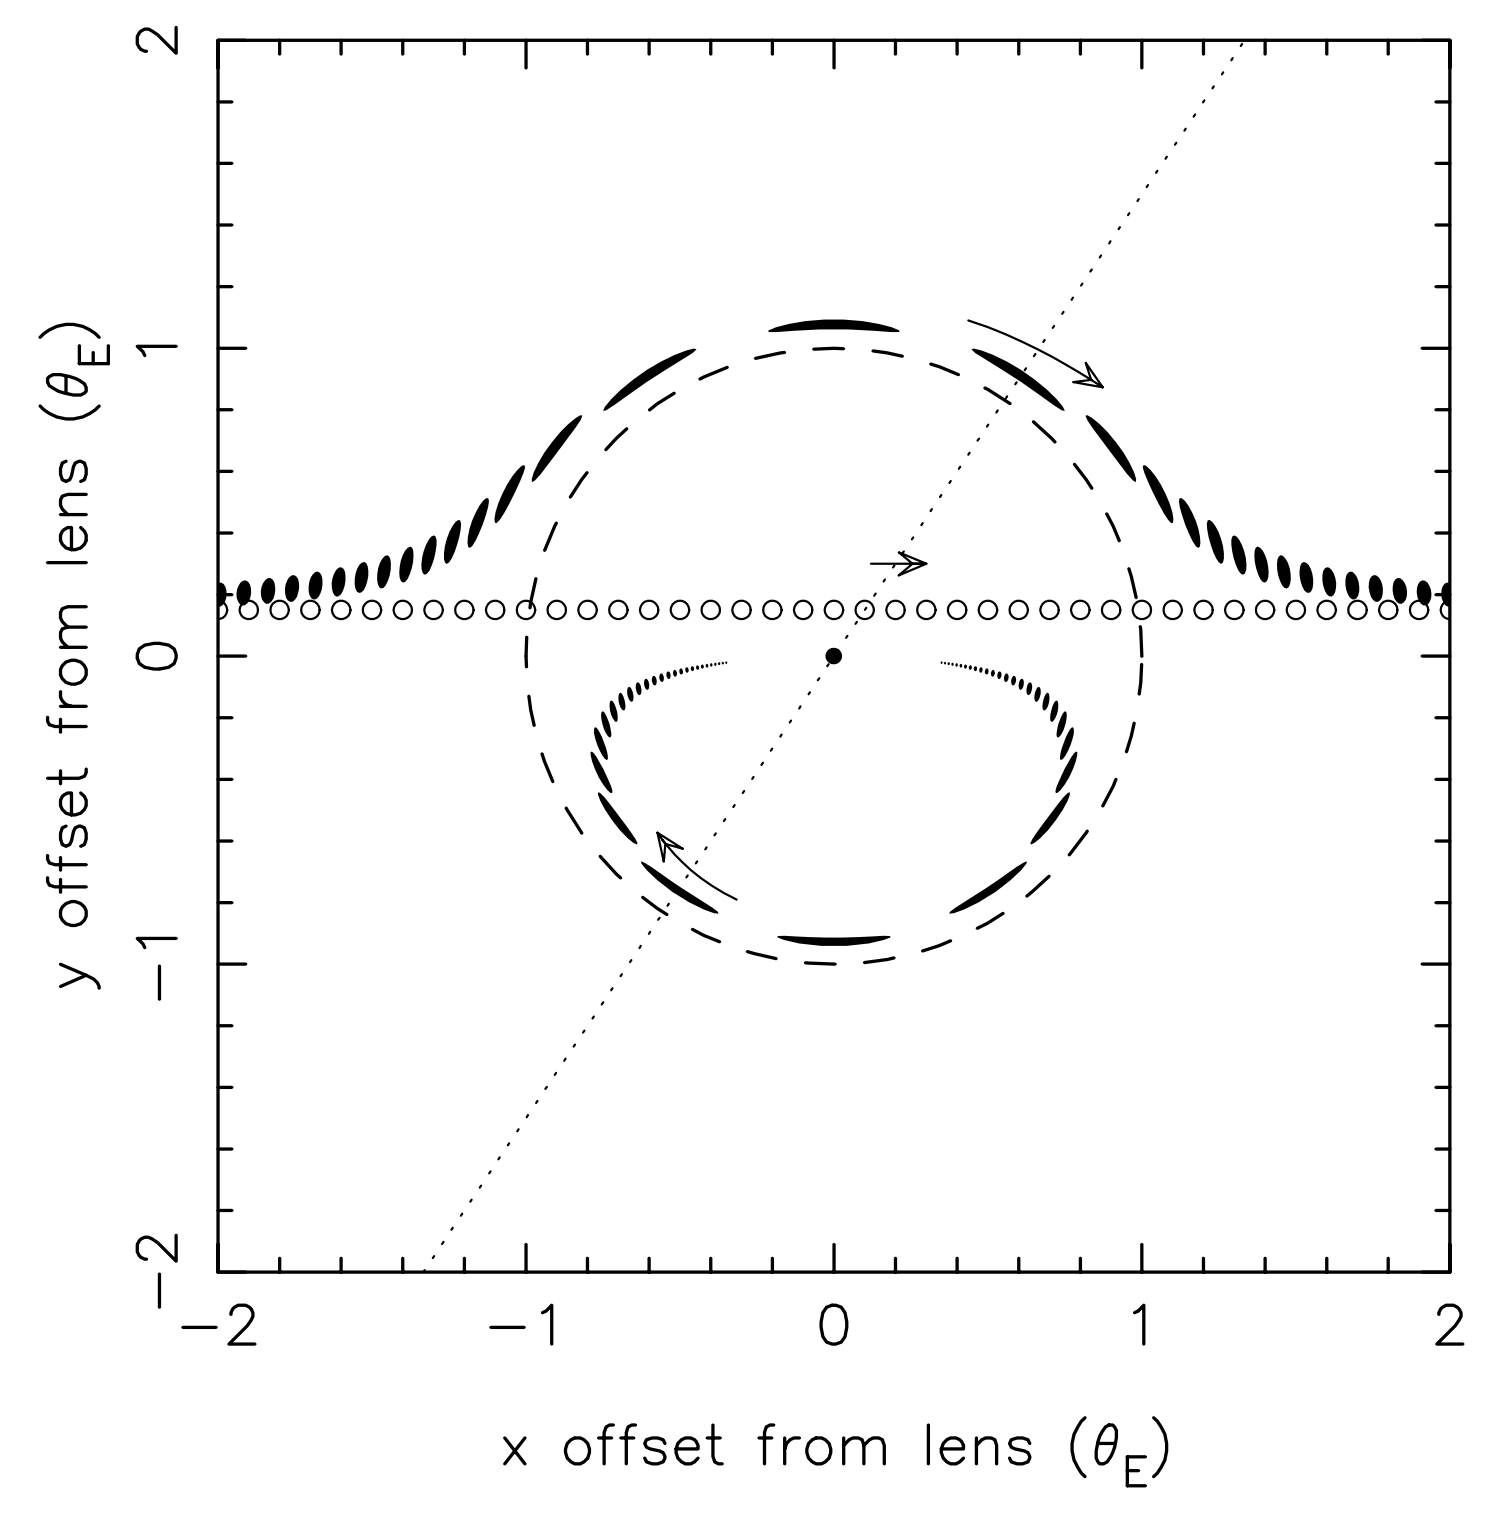
\includegraphics[width=6cm]{figures/microlensing.png}}
\end{figure}

{\noindent}Although the perfect alignment giving the Einstein ring will rarely occur in practice, it is still a very important concept because the size of the hypothetical Einstein ring sets the length scale over which substantial brightening will occur. As we will see, for a typical lens in our Galaxy the radius of the Einstein ring $r_E$ is roughly $8\sqrt{M/{\rm M_\odot}}\,{\rm AU}$, where $M$ is the lens mass. Knowing this scale allows us to understand most of the general characteristics of microlensing: it is extremely small compared with the typical distance to a lens, so the angular separation of the two images will be too small to resolve, hence the `micro'lensing. However, it is considerably larger than either the size of a star or the size of a MACHO, so we can usually approximate the lens and source as point-like, which leads to a simple prediction for the light curve shape. Also, $r_E$ is very small compared with the typical separation of objects in the Galaxy, which implies that microlensing will be a very rare phenomenon. Another notable feature is that $r_E$ is proportional to the square root of the lens mass. This means that the area of sky `covered' by a lens (at fixed distance) is proportional to its mass, so the total fraction of sky covered depends only on the total mass density in lenses, not the individual lens masses. This fraction is called the \textbf{optical depth} $\tau$, and is $\sim10^{-6}$ for Galactic microlensing. The duration for a microlensing event is given by the time for the lens to move by $2r_E$ relative to the Earth-star line; for typical Galactic speeds of $200\,{km\,s^{-1}}$, this is $\sim130\,{\rm days}\times\sqrt{M/{\rm M_\odot}}$.

{\noindent}For perfect alignment, simple geometry gives the (small) deflection angle of the light ray meeting Earth as $\alpha = r_E/d_L + r_E/(d_S-d_L)$, where $d_L$ is the observer–lens distance and $d_S$ is the source distance. Requiring this to equal the general relativity deflection, $\alpha=4GM/r_Ec^2$, we obtain

\begin{align*}
    r_E = \sqrt{\frac{4GMd_L}{c^2} \left(\frac{d_S-d_L}{d_S}\right)} ~ [{\rm AU}].
\end{align*}

{\noindent}The angular Einstein radius is just $\theta_E\equiv r_E/d_L$. If we now introduce a small offset of the lens by a distance $b$ from the Earth-source line (i.e., an angle $\delta\equiv b/d_L$, a simple generalization gives the two image angular positions (relative to the lens) as

\begin{align*}
    \theta_\pm = 0.5 \left[\delta\pm\sqrt{\delta^2+4\theta_E^2}\right] ~ [{\rm rad}].
\end{align*}

{\noindent}Since lensing preserves surface brightness, the magnification $A_i$ of each image is given by the ratio of image to source areas, which for a `small' source and any axisymmetric lens is just

\begin{align*}
    A_i = \left\lvert \frac{\theta_i}{\delta}\frac{{\rm d}\theta_i}{{\rm d}\delta} \right\rvert ~ [{\rm dimensionless}].
\end{align*}

{\noindent}For a point lens, this leads to a total observed magnification as the sum of the two image magnifications,

\begin{align*}
    A = A_+ + A_- = \frac{(\delta/\theta_E)^2+2}{(\delta/\theta_E)\sqrt{(\delta/\theta_E)^2+4}} ~ [{\rm dimensionless}].
\end{align*}

{\noindent}This behaves as $A\approx(\delta/\theta_E)^{-1}$ for $(\delta/\theta_)\lesssim0.5$, so the magnification may be large, but as $A\approx1+2(\delta/\theta_E)^{-4}$ for $(\delta/\theta_E)\gtrsim2$, so the magnification rapidly becomes negligible at large $(\delta/\theta_E)$. For uniform motions, we will have $(\delta/\theta_E)(t) = \sqrt{(\delta/\theta_E)_{\rm min}^2 + [v_\perp(t-t_0)/r_E]^2}$ where $v_\perp$ is the transverse velocity of the lens relative to the line of sight and $(\delta/\theta_E)_{\rm min}$ is the value of $(\delta/\theta_E)$ at closest approach, which occurs at time $t_0$. Substituting this into the equation for the magnitude $A$ gives the light curve $A(t)$; some examples are shown in Figure \ref{fig:microlensinglightcurve}.

\begin{figure}[t]
    \floatbox[{\capbeside\thisfloatsetup{capbesideposition={right,top},capbesidewidth=4cm}}]{figure}[\FBwidth]
    {\caption{\footnotesize{Microlensing event light curves (magnification versus time) for six values of the impact parameter $(\delta/\theta_E)_{\rm min}=0.0,0.2,...,1.0$ as labelled. Time is in units of the Einstein radius crossing time $r_E/v_\perp$. The inset illustrates the Einstein ring (dotted circle) and the source paths relative to the lens (dot) for the six curves. Figure taken from Encyclopedia of Astronomy and Astrophysics (2001).}}
    \label{fig:microlensinglightcurve}}
    {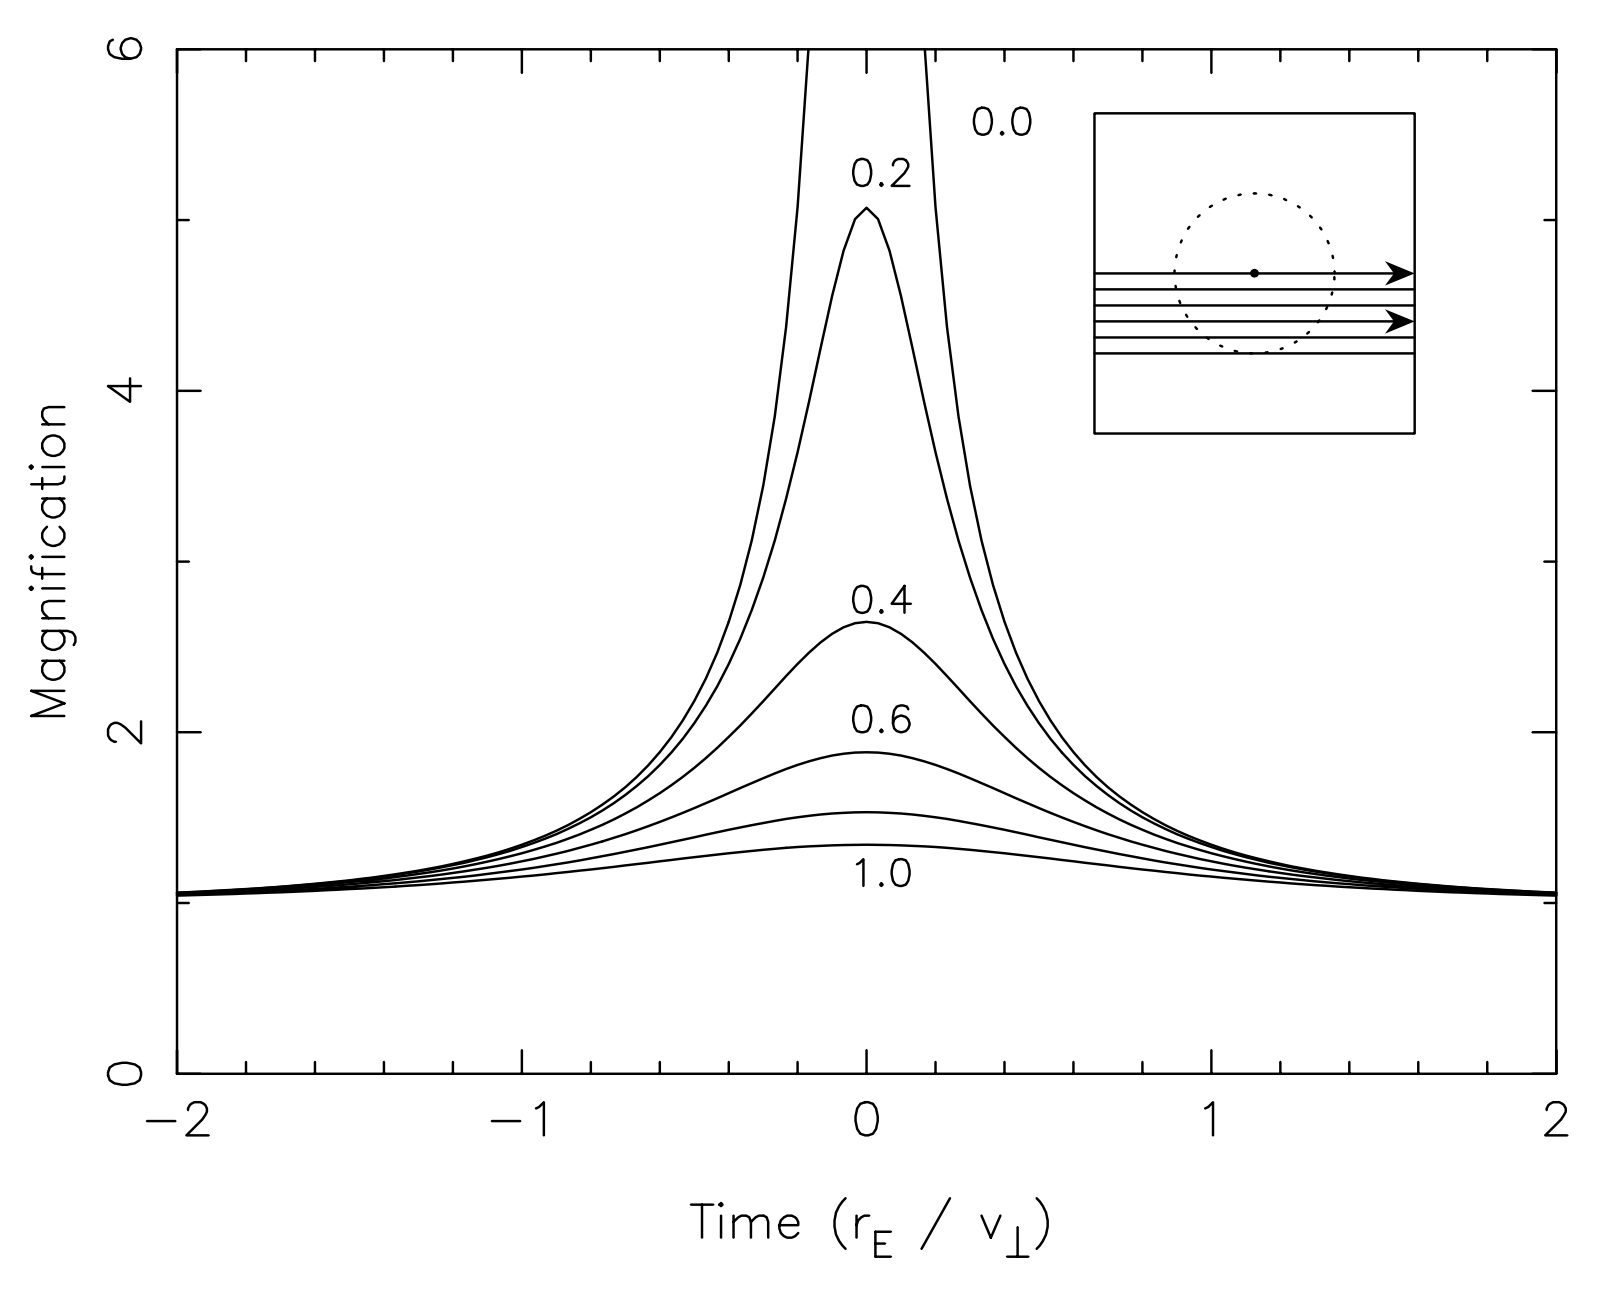
\includegraphics[width=10cm]{figures/MicrolensingLightcurve.png}}
\end{figure}

{\noindent}\textbf{Observations of microlensing}: To search for microlensing by MACHOs, since it is so rare we need millions of source stars and they should be far enough away to give a good path length for lensing, but not so far away that the individual stars  are faint. The obvious targets for dark-matter lenses are the LMC and SMC, the largest of our MW's many satellite galaxies, since the sight line to them passes mainly through the Galactic halo. The Galactic bulge is also an interesting target, although here because of the high stellar density the microlensing should be mainly due to intervening faint stars rather than dark matter. Around 1991, several teams of astronomers called MACHO, EROS and OGLE began large projects using wide-field $1\,{\rm m}$ class telescopes to search for microlensing events. The novel feature of these experiments is their massive data volume, requiring large amounts of disk and tape storage and special high-speed photometry programs. The expected number of microlensing events is much smaller than the fraction of intrinsic variable stars, but fortunately microlensing has many strong `signatures' that are distinct from all previously known types of variable star: the most important is the `uniqueness', (i.e., any given star should be microlensed at most once in a human lifetime), while almost all variable stars are periodic or quasi-periodic. Also, most events should have a symmetrical shape as in Figure \ref{fig:microlensinglightcurve}, and they should be achromatic (the source's colour should not change during the event), since lensing is independent of wavelength.

{\noindent}The MACHO, EROS and OGLE teams announced their first candidate microlensing events near simultaneously in late 1993 (Figure \ref{fig:microlensingcurve}). Since then, they have accumulated much more extensive datasets, and completed detailed calculations of their microlensing detection efficiency as a function of event duration; thus a number of general results have become clear:

\begin{enumerate}
    \item Hundreds of events have been observed towards the Galactic bulge. They are distributed `randomly' across the color-magnitude diagram, and their distribution of peak magnifications matches the theoretical prediction, which provides a very convincing check that microlensing works as predicted and that the experiments can detect it. The event rate towards the bulge is greater than initially predicted by Galactic models, favoring a barred structure for the Galaxy. The distribution of timescales is consistent with most of the lenses being low-mass stars as expected and can provide constraints on the stellar mass function at low masses.
    \item Towards the Magellanic Clouds, no `short' events (timescales from a few hours up to $20$ days) have been seen by any group. This places strong limits on `Jupiters' in the dark halo: specifically, compact objects in the mass range $10^{-6}-0.05\,{\rm M_\odot}$ contribute less than $10\%$ of the dark matter around our Galaxy. This is a very important result, as these objects were previously thought to be the most plausible form of baryonic DM, and (for masses below $0.01\,{\rm M_\odot}$) they would have been virtually impossible to detect directly.
    \item Approximately $18$ events with durations $30-200$ days have been observed towards the Magellanic Clouds. The implied optical depth is well above expectation from `known' stars, and is roughly $1/3$ of the value expected ($\tau\approx5\times10^{-7}$) for an all-MACHO dark halo. The relatively long durations imply lens masses of roughly $0.3-0.7\,{\rm M_\odot}$, which is a puzzle.
    \item Many events are now detected in real time and announced on the world-wide web. This enables more frequent monitoring of ongoing events, giving more precised tests of the shape. This has attracted considerable interest since, where the lens is a low-mass star (probably the case for most of the events towards the Galactic bulge), a planet around the lens star may give rise to a short-duration `blip' superimposed on the smooth microlensing light curve: this method is potentially sensitive to low-mass planets down to a few Earth masses, below the range accessible to radial-velocity planet searches. Two groups called PLANET and MPS are now searching for this effect.
\end{enumerate}

\begin{figure}[t]
    \floatbox[{\capbeside\thisfloatsetup{capbesideposition={right,top},capbesidewidth=4cm}}]{figure}[\FBwidth]
    {\caption{\footnotesize{\\The first LMC microlensing candidate from the MACHO project. (Expanded view: $6\,{\rm yr}$ of constant data are outside the plot). Upper and middle panels show brightness versus time in blue and red passbands respectively, in units of the baseline value. Points with error bars are observations, the curve is the best microlensing fit. The lower panel shows the ratio of red/blue flux, illustrating the lack of color change. Figure taken from Encyclopedia of Astronomy and Astrophysics (2001).}}
    \label{fig:microlensingcurve}}
    {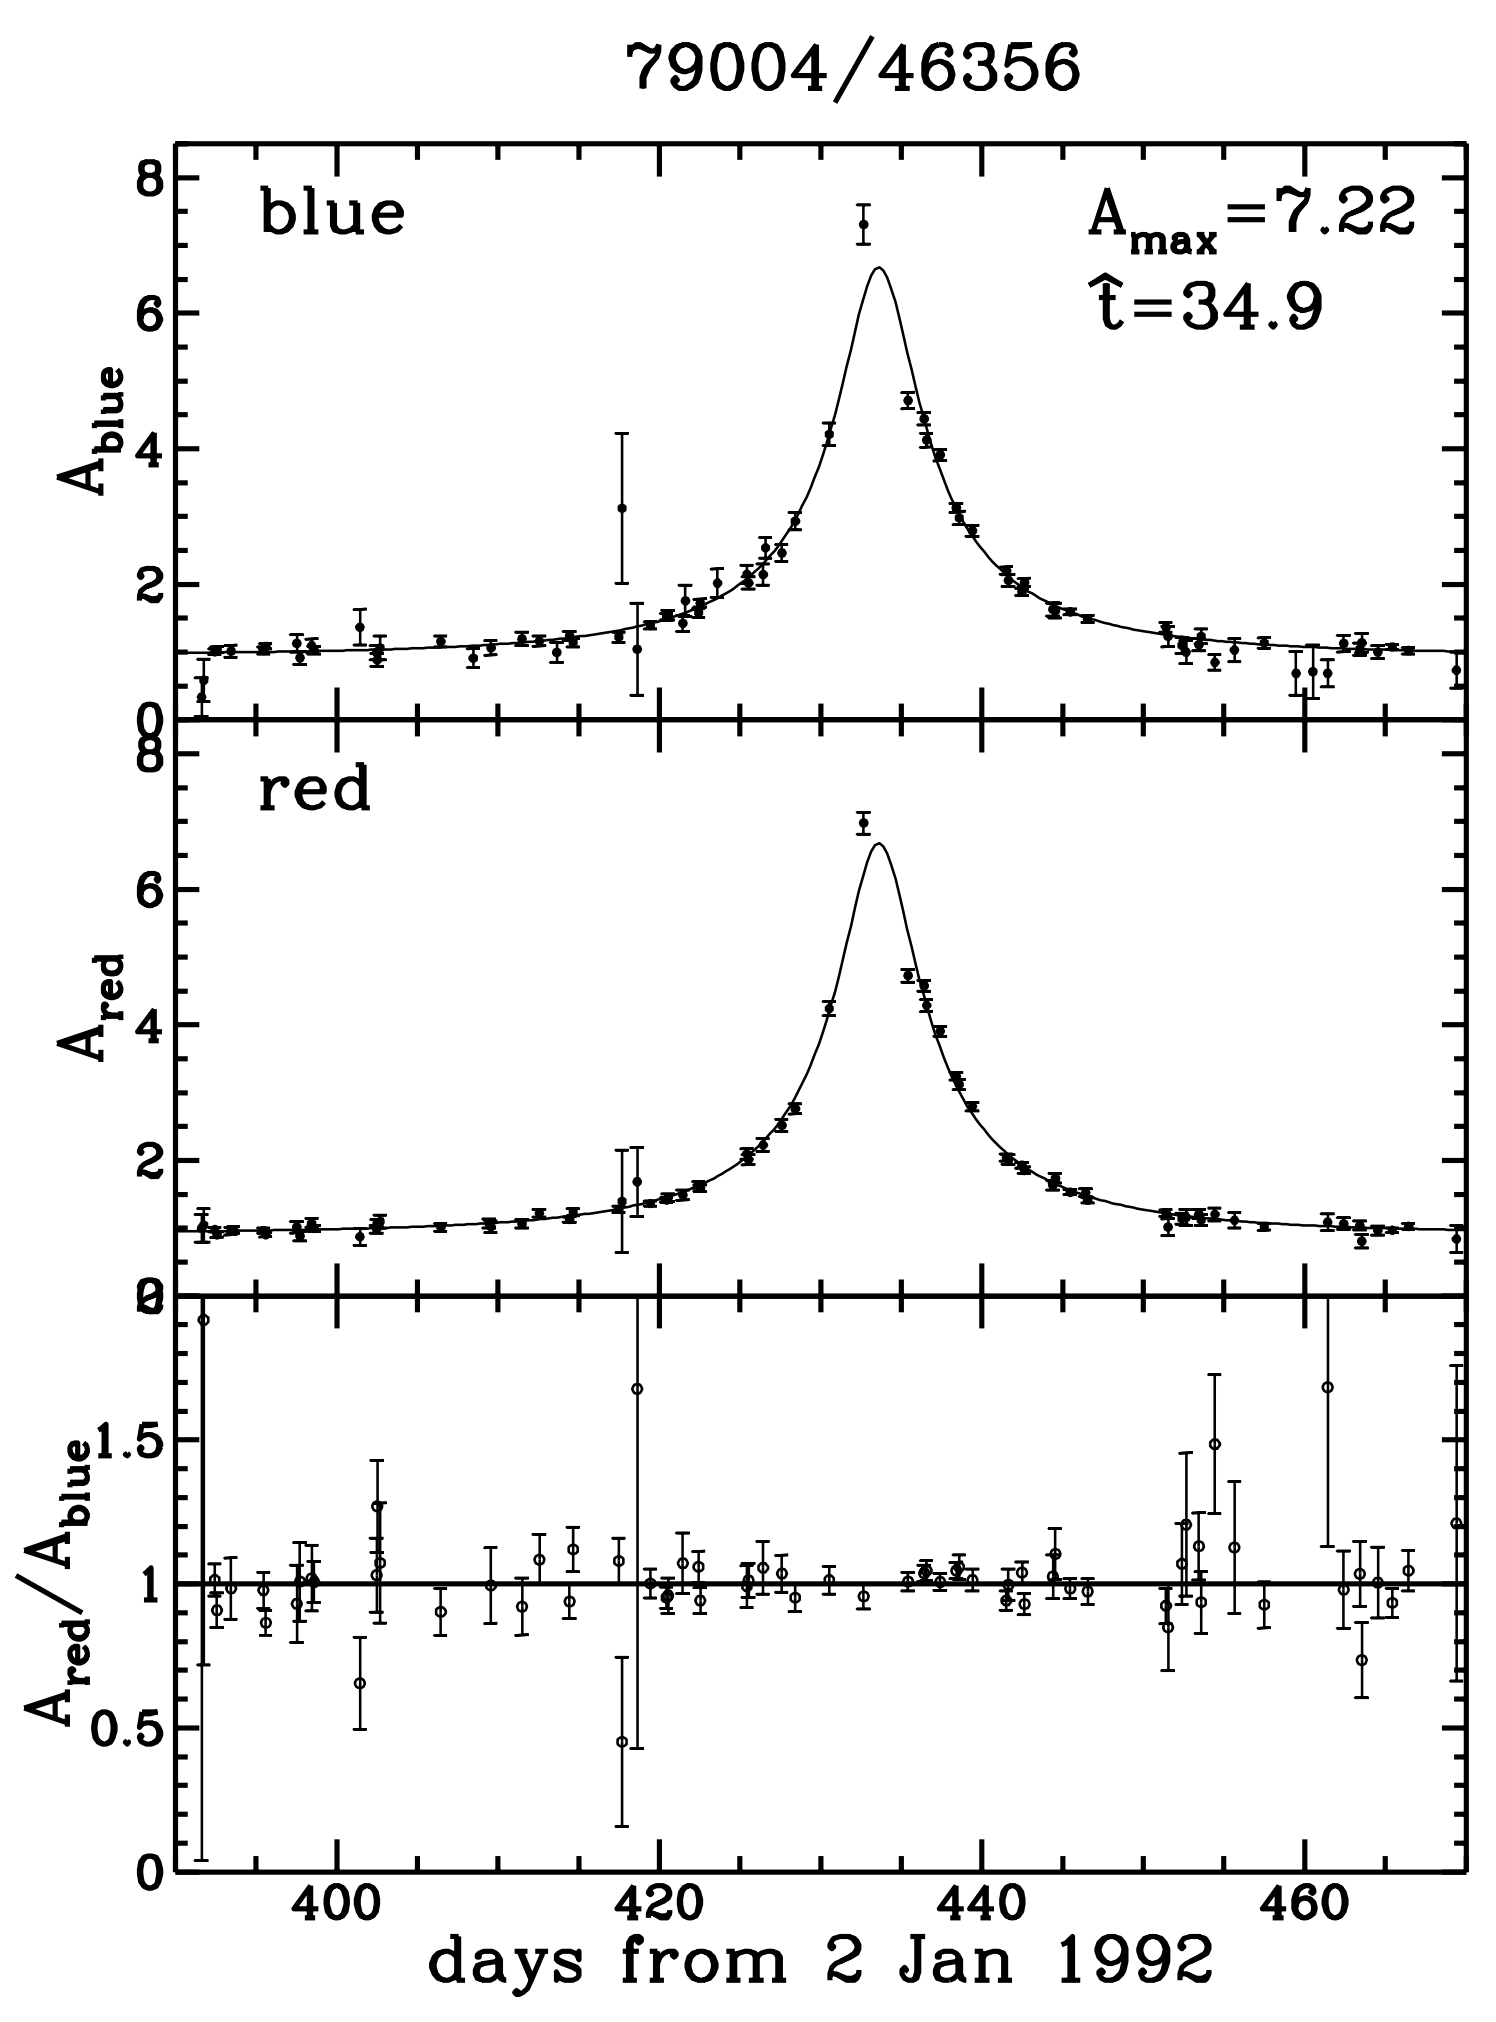
\includegraphics[width=8cm]{figures/MicrolensingCurve.png}}
\end{figure}

{\noindent}\textbf{Current questions in microlensing}: The nature of the objects giving rise to the lensing towards the Magellanic Clouds is a significant puzzle at present; the inferred lens masses are well above $0.1\,{\rm M_\odot}$, which means that they cannot be ordinary hydrogen-burning stars in a spherical halo, as these would be visible in large numbers in deep images (e.g., the Hubble Deep Field). There are two classes of solution: either the lenses are in the halo but are much fainter (e.g., old white dwarfs or possibly primordial black holes), or they are low-mass stars but in a non-halo population (i.e., preferentially concentrated in the foreground of the LMC). The white-dwarf solution has significant problems associated with early metal production but has received some support recently from a possible detection of proper motions of faint objects in the Hubble Deep Field. Various classes of non-halo population have been proposed (e.g., a `thick' LMC disk, a small dwarf galaxy projected in front of the LMC, a warped Milky Way disk etc.), but several searches for such populations have been negative.

{\noindent}There are several ways of testing these possibilities: one is to measure distances to individual lenses. In a `standard' microlensing event as in Figure \ref{fig:microlensinglightcurve} it is impossible to measure the lens distance since the one physical parameter (event duration) depends on three unknowns, the lens mass, distance, and transverse velocity. However, as proposed by Gould and others, a small fraction of observed events should deviate from the standard shape for one of several reasons: the non-uniform motion of the Earth, the finite size of the source, a binary lens etc. In these cases we can obtain an additional observable which constrains the location of the lens. At present there are only one or two such cases for Magellanic Cloud lensing. Future satellite observations may help to measure lens distances, either by measuring the `parallax' effect or the small centroid shift during the event.

{\noindent}Another active area is the search for microlensing towards the Andromeda galaxy, M31. This is considerably more challenging since the greater distance means that there are multiple unresolved stars per resolution element, and sophisticated image differencing techniques are necessary. However, it has the advantage that microlensing from M31's own halo will produce substantially more events towards the far side of M31's disk than towards the near side, owing to the nearly edge-on inclination. Two groups called AGAPE and MEGA have done pilot studies and are currently undertaking large-scale searches towards M31.

{\noindent}\textbf{Cosmological microlensing}: Although microlensing within the Local Group is the main application at present, microlensing of `point' sources at cosmological distances (e.g., QSOs, SNe, or gamma-ray bursts) may also be observable. In the case of a QSO lensed into multiple images by a foreground galaxy, the individual stars in the galaxy may act as microlenses. Here the microlensing appears as brightness changes unique to one image of the multiplet (after correcting for the time delay); in this case the optical depth is typically close to unity (because the surface density must be of order the `critical' surface density to produce multiple imaging), so the interpretation of the light curve is complex. Other searches are in progress for microlensing of quasars behind the Virgo Cluster by dark objects in the cluster, and the Next Generation Space Telescope should be easily able to detect microlensing of stars in the Virgo galaxy M87.

\subsubsection{Follow-up Questions}

\begin{itemize}
    \item Can you derive $\alpha$ from a Newtonian approach?
    \item Why/how does gravitational lensing magnify a star?
\end{itemize}

% --------------------------------------------------------------
%               2. 
% --------------------------------------------------------------

\newpage
\subsection{Question 2}

A two-element interferometer consists of two telescopes whose light is combined and interfered. Sketch the response of such an interferometer to a nearby red giant star, as a function of the (projected) separation between the two telescopes. The red giant subtends one-fiftieth of an arc second on the sky, and the telescope operates at a wavelength of 2 microns.

\subsubsection{Short answer}

Answer.

\subsubsection{Additional context}

{\noindent}\textbf{The two-element quasi-monochromatic interferometer}: The simplest radio interferometer is a pair of radio telescopes whose voltage outputs are correlated (multiplied and averaged), and even the most elaborate interferometers with $N\gg2$ antennas, often called \textbf{elements}, can be treated as $N(N-1)/2$ independent two-element interferometers. Figure \ref{fig:radiointerferometer} shows two identical dishes separated by the \textbf{baseline vector} $\vec{b}$ of length $b$ that points from antenna $1$ to antenna $2$. Both dishes point in the same direction specified by the unit vector $\hat{s}$, and $\theta$ is the angle between $\vec{}b$ and $\hat{s}$. Plane waves from a distant point source in this direction must travel an extra distance $\vec{b}\cdot\hat{s}=b\cos\theta$ to reach antenna $1$, so the output of antenna $1$ is the same as that of antenna $2$, but it lags in time by the geometric delay

\begin{align*}
    \tau_g = \frac{\vec{b}\cdot\hat{s}}{c} ~ [{\rm s}].
\end{align*}

{\noindent}For simplicity, we first consider a quasi-monochromatic interferometer, one that responds only to radiation in a very narrow band $\Delta\nu\ll2\pi/\tau_g$ centered on frequency $\nu=\omega/(2\pi)$. Then the output voltages of antennas $1$ and $2$ at time $t$ can be written as

\begin{align*}
    V_1 &= V\cos[\omega(t-\tau_g)] ~ [{\rm V}] \\
    V_2 &= V\cos(\omega t) ~ [{\rm V}].
\end{align*}

{\noindent}These output voltages are amplified versions of the antenna input voltages; they have not passed through square-law detectors. Instead, a \textbf{correlator} multiplies these two voltages to yield the product

\begin{align*}
    V_1V_2 = V^2\cos[\omega(t-\tau_g)]\cos(\omega t) = \left(\frac{V^2}{2}\right) [\cos(2\omega t-\omega \tau)g)+\cos(\omega\tau_g)] ~ [{\rm V}]
\end{align*}

{\noindent}which follows directly from the trigonometric identity $\cos x\cos y = [\cos(x+y)+\cos(x-y)]/2$. The correlator also takes a time average long enough ($\Delta t\gg(2\omega)^{-1}$) to remove the high-frequency term $\cos(2\omega t-\omega\tau_g)$ from the \textbf{correlator response} (output voltage) $R$ and keep only the slowly varying term

\begin{align*}
    R = \langle V_1V_2 \rangle = \left(\frac{V^2}{2}\right)\cos(\omega\tau_g) ~ [{\rm V^2}].
\end{align*}

{\noindent}The voltages $V_1$ and $V_2$ are proportional to the electric field produced by the source multiplied by the voltage gains of the two antennas and receivers. Thus the correlator output amplitude $V^2/2$ is proportional to the flux density $S$ of the point source multiplied by $\sqrt{A_1A_2}$, where $A_1$ and $A_2$ are the effective collecting areas of the two antennas.

{\noindent}Notice that the time-averaged response $R$ of a multiplying interferometer is zero. There is no DC output, so fluctuations in receiver gain do not act on the whole system temperature $T_s$ as for a total-power observation with a single dish. Uncorrelated noise power from very extended radio sources such as the CMB and the atmosphere over the telescopes, also averages to zero in the correlator response. Short interference pulses with duration $t\ll \lvert b\rvert/c$ are also suppressed because each pulse does not reach both telescopes simultaneously. Likewise, a multiplying radio interferometer differs from a classical \textbf{adding interferometer}, such as the optical Michelson interferometer, that adds the uncorrelated noise power contributions.

{\noindent}The correlator output voltage $R=(V^2/2)\cos(\omega\tau_g)$ varies sinusoidally as the Earth's rotation changes the source direction relative to the baseline vector. These sinusoids are called \textbf{fringes}, and the \textbf{fringe phase}

\begin{align*}
    \phi = \omega\tau_g = \frac{\omega}{c} b\cos\theta ~ [{\rm rad}]
\end{align*}

{\noindent}depends on $\theta$ as follows:

\begin{align*}
    \frac{{\rm d\phi}}{{\rm d}\theta} = \frac{\omega}{c} b\sin\theta = 2\pi \left(\frac{b\sin\theta}{\lambda}\right) ~ [{\rm dimensionless}].
\end{align*}

\begin{figure}[t]
    \floatbox[{\capbeside\thisfloatsetup{capbesideposition={right,top},capbesidewidth=6cm}}]{figure}[\FBwidth]
    {\caption{\footnotesize{This block diagram shows the components of a two-element quasi-monochromatic \textbf{multiplying interferometer} observing in a very narrow radio frequency range centered on $\nu=\omega/(2\pi)$. $\hat{s}$ is the unit vector in the direction of a distant point source and $\vec{b}$ is the baseline vector pointing from antenna $1$ to antenna $2$. The output voltage $V_1$ of antenna $1$ is the same as the output voltage $V_2$ of antenna $2$, but it is retarded by the geometric delay $\tau_g=\vec{b}\cdot\hat{s}/c$ representing the additional light-travel delay to antenna $1$ for a plane wavefront from a source at angle $\theta$ from the \textbf{baseline vector}. These voltages are amplified, multiplied ($\times$), and time averaged ($\vert\rvert$) by the \textbf{correlator} to yield an output response whose amplitude $R$ is proportional to the flux density of the point source and whose phase ($\omega\tau_g$) depends on the delay and the frequency. The quasi-sinusoidal output \textbf{fringe} shown occurs if the source direction in the interferometer frame is changing at a constant rate ${\rm d}\theta/{\rm d}t$. The broad Gaussian envelope of the fringe shows the primary-beam attenuation as the source passes through the beam of the dishes. Figure taken from Condon \& Random (2016).}}
    \label{fig:radiointerferometer}}
    {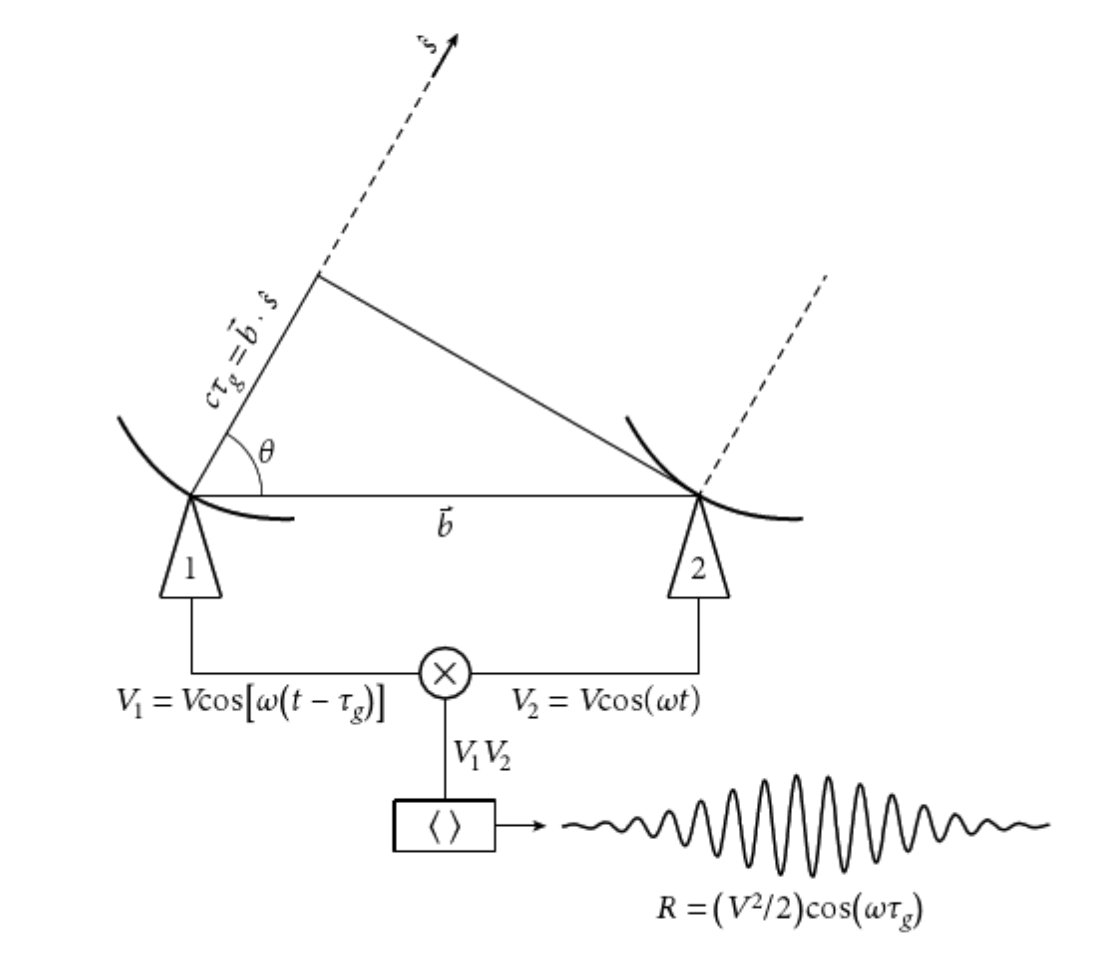
\includegraphics[width=10cm]{figures/RadioInterferometer.png}}
\end{figure}

{\noindent}The \textbf{fringe period} $\phi=2\pi$ corresponds to an angular shift $\theta=\lambda/(b\sin\theta)$. The fringe phase is an exquisitely sensitive measure of source position if the \textbf{projected baseline} $b\sin\theta$ is many wavelengths long. Note that fringe phase and hence measured source position is not affected by small tracking errors of the individual telescopes. It depends on time, and times can be measured by clocks with much higher accuracy than angles (ratios of lengths of moving telescope parts) can be measured by rulers. Also, an interferometer whose baseline is horizontal is not affected by the plane-parallel component of atmospheric refraction, which delays the signals reaching both telescopes equally. Consequently, interferometers can determine the positions of compact radio sources with unmatched accuracy. Absolute positions with errors as small as $\sigma_\theta\approx10^{-3}\,{\rm arcsec}$ and differential positions with errors down to $\sigma_\theta\approx10^{-5}\,{\rm arcsec}<10^{-10}\,{\rm rad}$ have frequently been measured.

{\noindent}If the individual antennas comprising an interferometer were isotropic, the interferometer point-source response would be a sinusoid spanning the sky. Such an interferometer is sensitive to only one Fourier component of the sky brightness distribution: the component with angular period $\lambda/(b\sin\theta$). The response $R$ of a two-element interferometer with directive antennas is that sinusoid multiplied by the product of the voltage patterns of the individual antennas. Normally the two antennas are identical, so this product is the power pattern of the individual antennas and is called the \textbf{primary beam} of the interferometer. The primary beam is usually a Gaussian much wider than a fringe period, as indicated in Figure \ref{fig:radiointerferometer}. The convolution theorem states that the Fourier transform of the product of two functions is the convolution of their Fourier transforms, so the interferometer with directive antennas responds to a finite range of angular frequencies centered on $b\sin\theta/\lambda$. Because the antenna diameters $D$ must be smaller than the baseline $b$ (else the antennas would overlap), the angular frequency response cannot extend to zero and the interferometer cannot detect an isotropic source -- the bulk of the $3\,{\rm K}$ CMB for example. The missing short spacings ($b<D$) can be provided by a single-dish telescope with diameter $D>b$. Thus the $D=100\,{\rm m}$ GBT can fill in the missing baselines $b<25\,{\rm m}$ that the $D=25\,{\rm m}$ VLA dishes cannot obtain.

{\noindent}Improving the instantaneous point-source response pattern of an interferometer requires more Fourier components; that is, more baselines. An interferometer with $N$ antennas contains $N(N-1)/2$ pairs of antennas, each of which is a two-element interferometer, so the instantaneous \textbf{synthesized beam} (the point-source response obtained by averaging the outputs of all of the two-element interferometers) rapidly approaches a Gaussian as $N$ increases. The instantaneous point-source responses of a two-element interferometer with projected baseline length $b$, a three-element interferometer with three baselines (projected lengths $b/3,2b/3$, and $b$), and a four-element interferometer with six baselines (projected lengths $b/6,2b/6,3b/6,4b/6,5b/6$, and $b$) are shown in Figure \ref{fig:interferometerbeam}.

{\noindent}Most radio sources are stationary; that is, their brightness distributions do not change significantly on the timescales of astronomical observations. For stationary sources, a two-element interferometer with movable antennas could make $N(N-1)/2$ observations to duplicate one observation with an $N$-element interferometer.

\begin{figure}[t]
    \floatbox[{\capbeside\thisfloatsetup{capbesideposition={right,top},capbesidewidth=6cm}}]{figure}[\FBwidth]
    {\caption{\footnotesize{The instantaneous point-source responses of interferometers with overall projected length $b$ and two, three, or four antennas distributed as shown are indicated by the thick curves. The synthesized main beam of the four-element interferometer is nearly Gaussian with angular resolution $\theta\approx\lambda/b$, but the sidelobes are still significant and there is a broad negative ``bowl'' caused by the lack of spacings shorter than the diameter of an individual antenna. Thus the \textbf{synthesized beam} is sometimes called the \textbf{dirty beam}. The instantaneous dirty beam of the multi-element interferometer is the arithmetic mean of the individual responses of its component two-element interferometers. The individual responses of the three two-element interferometers comprising the three-element interferometer and of the six two-element interferometers comprising the four-element interferometer are plotted as thin curves. Figure taken from Condon \& Random (2016).}}
    \label{fig:interferometerbeam}}
    {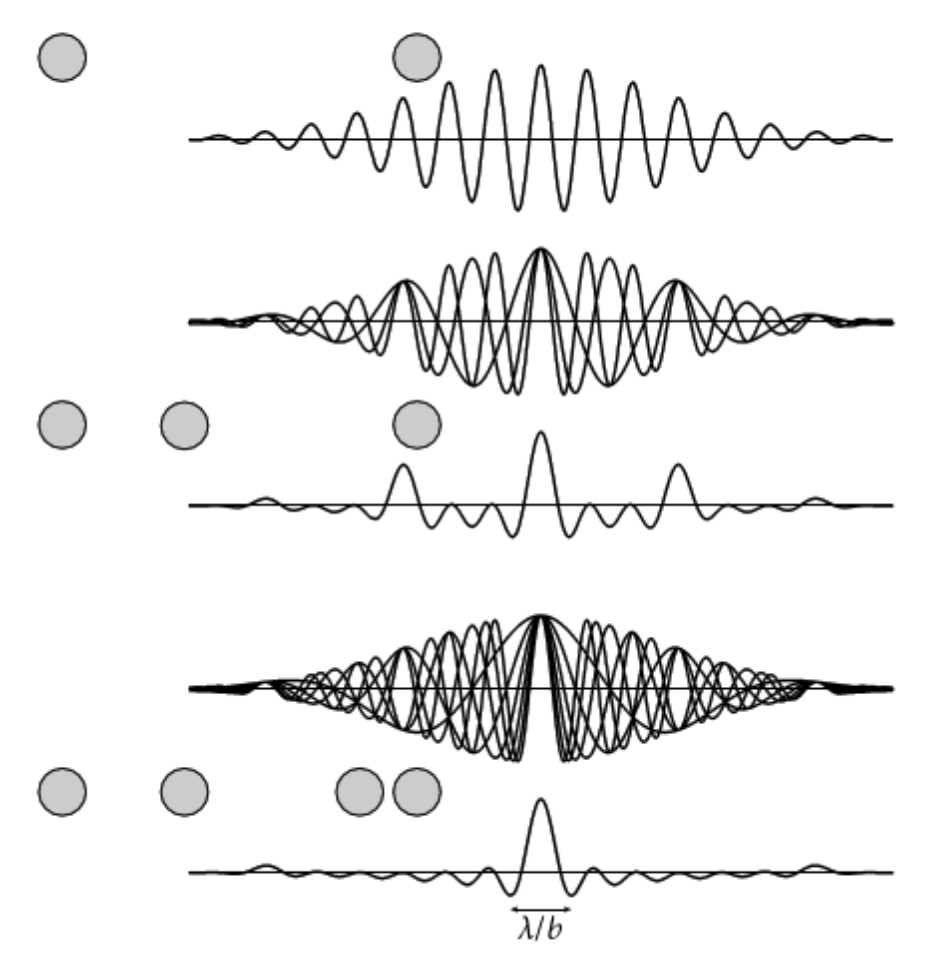
\includegraphics[width=10cm]{figures/InterferometerBeam.png}}
\end{figure}

{\noindent}\textbf{Slightly extended sources and the complex correlator}: The response $R=(V^2/2)\cos(\omega\tau_g)$ of the quasi-monochromatic two-element interferometer with a ``cosine'' correlator (Figure \ref{fig:radiointerferometer}) to a spatially incoherent slightly extended (much smaller than the primary beamwidth) source with sky brightness distribution $I_\nu(\hat{s})$ near frequency $\nu=\omega/(2\pi)$ is obtained by treating the extended source as the sum of independent point sources:

\begin{align*}
    R_c = \int I(\hat{s})\cos(2\pi\nu\vec{b}\cdot\hat{s}/c){\rm d}\Omega = \int I(\hat{s})\cos(2\pi\vec{b}\cdot\hat{s}/\lambda){\rm d}\Omega ~ [{\rm V^2}].
\end{align*}

{\noindent}Notice that the even cosine function in this response is sensitive only to the even (inversion-symmetric) part $I_E$ of an arbitrary source brightness distribution, which can be written as the sum of even and odd (anti-symmetric) parts: $I=I_E+I_O$. To detect the odd part $I_O$ we need a ``sine'' correlator whose output is odd, $R=(V^2/2)\sin(\omega\tau_g)$. This can be implemented by a second correlator that follows a $\pi/2\,{\rm rad}=90^\circ$ phase delay inserted into the output of one antenna because $\sin(\omega\tau_g)=\cos(\omega\tau_g-\pi/2)$. Then

\begin{align*}
    R_s = \int I(\hat{s})\sin(2\pi\vec{b}\cdot\hat{s}/\lambda){\rm d}\Omega ~ [{\rm V^2}]
\end{align*}

{\noindent}The combination of cosine and sine correlators is called a \textbf{complex correlator} because it is mathematically convenient to treat the cosines and sines as complex exponentials using Euler's formula

\begin{align*}
    e^{i\phi} = \cos\phi + i\sin\phi ~ [{\rm rad}].
\end{align*}

{\noindent}The \textbf{complex visibility} is defined by

\begin{align*}
    \mathcal{V} \equiv R_c - i R_s ~ [{\rm V^2}]
\end{align*}

{\noindent}which can be written in the form

\begin{align*}
    \mathcal{V} = Ae^{-i\phi} ~ [{\rm rad}],
\end{align*}

{\noindent}where 

\begin{align*}
    A = \sqrt{R_c^2 + R_s^2} ~ [{\rm dimensionless}]
\end{align*}

{\noindent}is the \textbf{visibility amplitude} and

\begin{align*}
    \phi = \arctan \left(\frac{R_s}{c}\right) ~ [{\rm rad}]
\end{align*}

{\noindent}is the \textbf{visibility phase}. The response to an extended source with brightness distribution $I(\hat{s})$ of the two-element quasi-monochromatic interferometer with a complex correlator is the complex visibility

\begin{align*}
    \mathcal{V} = \int I(\hat{s}) \exp (-i2\pi\vec{b}\cdot\hat{s}/\lambda){\rm d}\Omega ~ [{\rm V^2}].
\end{align*}

{\noindent}\textbf{Fringe patterns and Fourier transforms}: Interferometry begins with the Young’s slits fringe pattern (Fig. 1). With a single point source emitting coherent radiation, interference fringes are observed, with constructive and destructive interference observed as the relative delay of the two interfering rays changes; the separation of the fringes is λ/d, the wavelength of the light divided by the slit separation.

\begin{figure}[t]
    \floatbox[{\capbeside\thisfloatsetup{capbesideposition={right,top},capbesidewidth=5cm}}]{figure}[\FBwidth]
    {\caption{\footnotesize{Young's slits in various situations. In each panel the source is shown on the left, and on the right of the slit are shown the fringe patterns separately for each part of the source and then the added fringe pattern. \textbf{(a)}: The basic two-slit pattern, showing fringes an angular distance $\lambda/d$ apart. \textbf{(b)}: The effect of increasing the source size. An angular shift of the source position by $\theta$ shifts the fringe patterns by $\theta$ the other way. Since the patterns come from mutually incoherent sources, the intensity patterns add to give a pattern of reduced visibility. \textbf{(c)}: When the size of the source reaches $\lambda/d$, the fringes add to give zero visibility. \textbf{(d)}: If the slit spacing is then reduced, the fringe spacing increases, and the same size of source is still able to give visible fringes: the source would need to be increased in size to $\lambda/d_{\rm new}$ in order to wash out the fringes. Figure taken from Jackson.}}
    \label{fig:slitpatterns}}
    {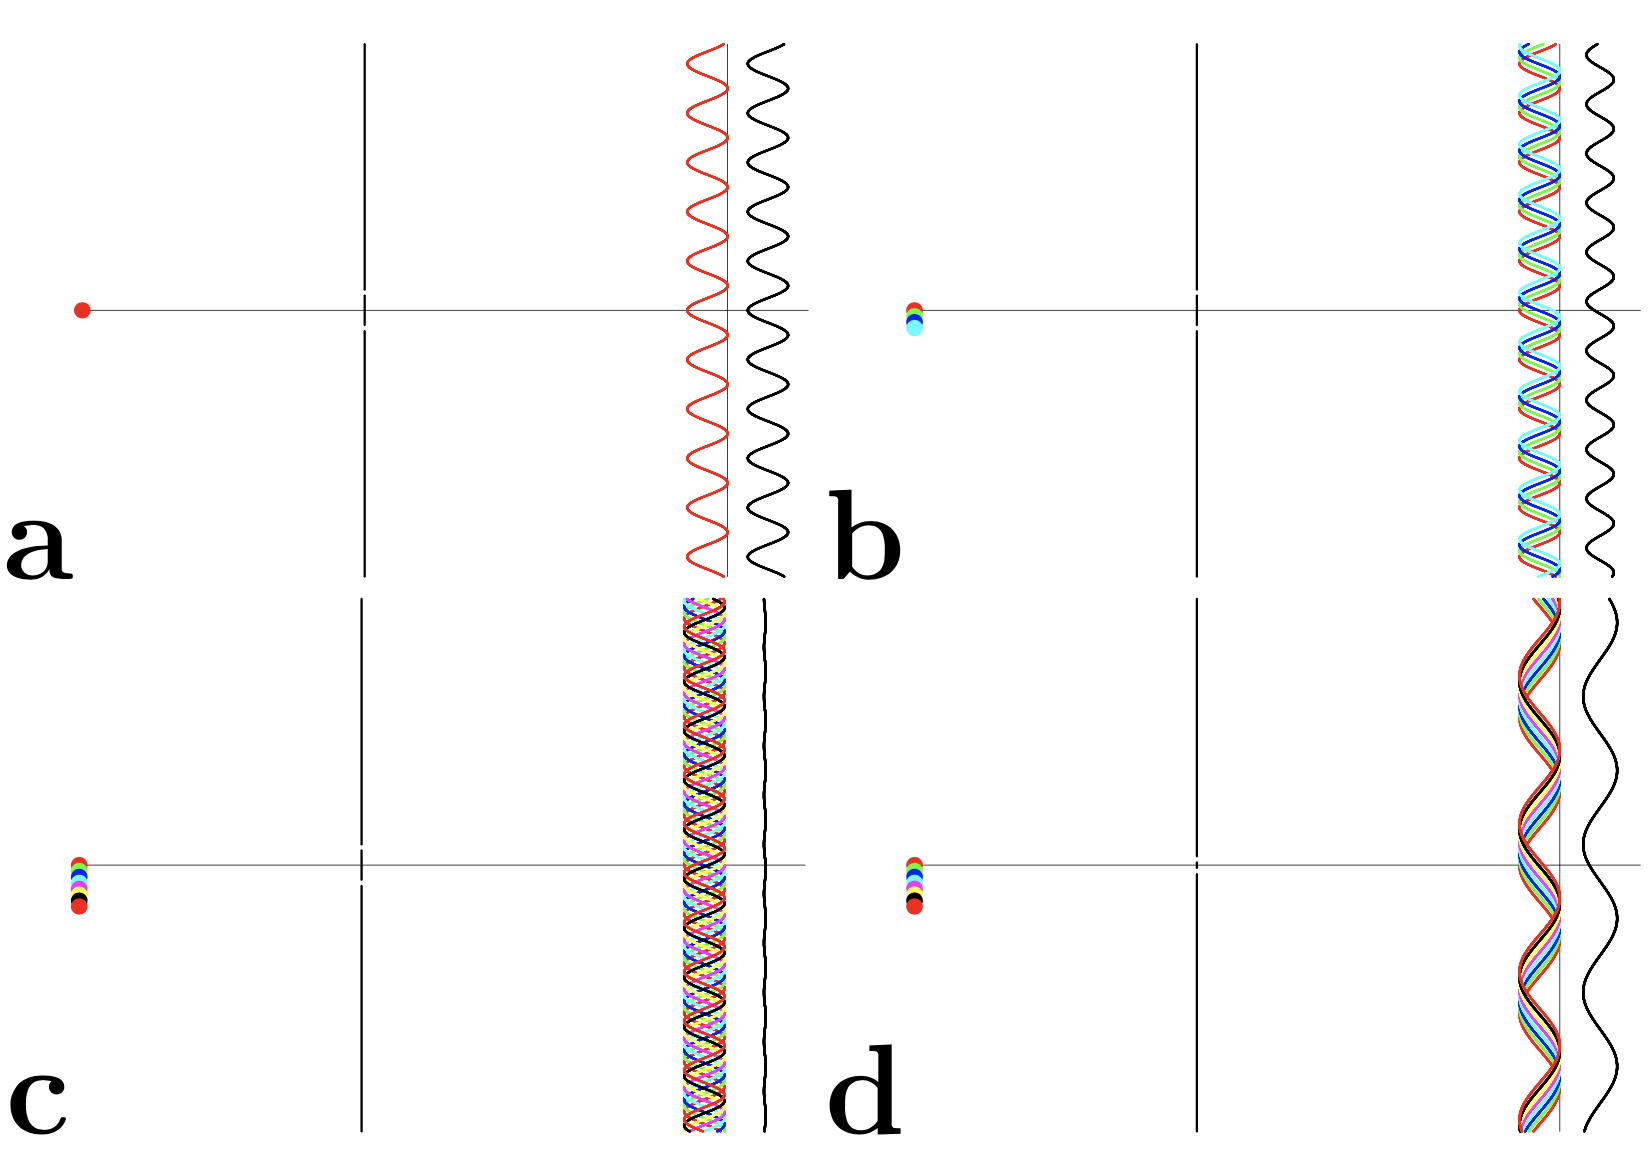
\includegraphics[width=10cm]{figures/SlitPatterns.png}}
\end{figure}

{\noindent}If the source is made wider (Figure \ref{fig:slitpatterns}b), we can think of it as a sequence of point sources each of which emit radiation which is uncorrelated with the emission from the others. It follows that the total interference intensity pattern is the sum of the individual patterns. Since an angular displacement in the source produces an equal angular displacement in the fringe pattern, as the source size approaches $\lambda/d$ the fringe patterns will add to give a constant illumination (Figure \ref{fig:slitpatterns}c). In this case, the fringe visibility (defined as the difference between maximum and minimum intensity, normalized by the sum of maximum and minimum intensity) drops to zero. Conversely, when the angular size of the source is $\lambda/d$, the fringe visibility is $1$; this corresponds to a situation in which the source size is smaller than the angular resolution of the interferometer, and only an upper limit of order $\lambda/d$ can be obtained on it.

{\noindent}Now suppose that the slit spacing $d$ is decreased. For the same size of source, this produces less ``washing-out'' of the fringes, because the same displacement of the source now produces much less displacement of the fringe patterns as a fraction of the fringe separation $\lambda/d$ (Figure \ref{fig:slitpatterns}d). The smaller the slit separation, the larger the source size that can be probed using interferometry.

{\noindent}The situation is summarized in Figure \ref{fig:fringevisibility}. If we plot, for a given source distribution, the way in which visibility varies with slit separation, it can be seen that for small sources the visibility remains high out to large slit separation (in the limit of point sources, to infinite slit separation), whereas large sources produce visibility patterns which fall off quickly as the slit separation increases.

{\noindent}The relation between $I(\theta)$ and $V(d)$ represented here is one which maps a
large Gaussian into a small Gaussian, and vice versa, and it is fairly obvious that it is a Fourier transform\footnote{This is known as the Van \textbf{Cittert-Zernicke theorem}.}.

discussion that follows.

\begin{figure}[t]
    \floatbox[{\capbeside\thisfloatsetup{capbesideposition={left,top},capbesidewidth=4cm}}]{figure}[\FBwidth]
    {\caption{\footnotesize{\\Relation between source brightness as a function of angular distance and visibility of interference fringes as a function of slit separation (baseline length). Figure taken from Jackson.}}
    \label{fig:fringevisibility}}
    {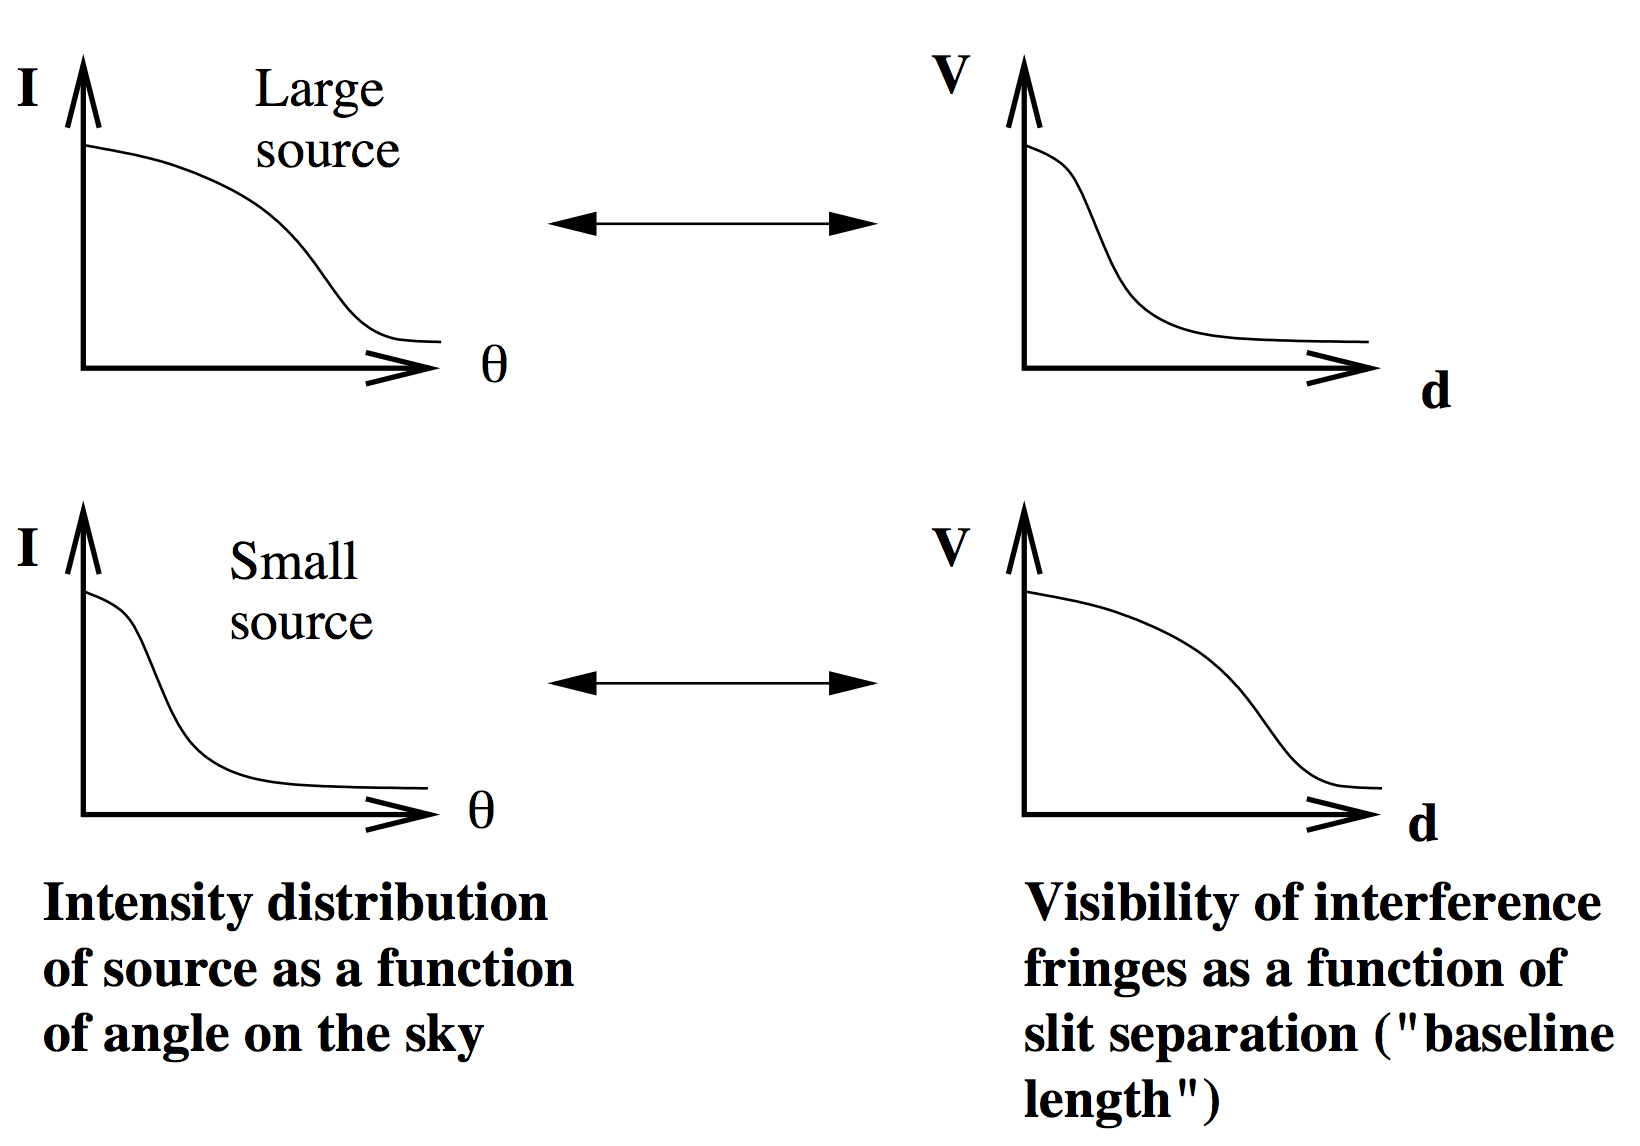
\includegraphics[width=12cm]{figures/FringeVisibility.png}}
\end{figure}

\newpage
\subsubsection{Follow-up Questions}

\begin{itemize}
    \item What do the minima in the response function tell you?
\end{itemize}

% --------------------------------------------------------------
%               3. 
% --------------------------------------------------------------

\newpage
\subsection{Question 3}

What's the minimum mass of a black hole you could survive a fall through the event horizon without being ripped to shreds? Why would you be ripped to shreds for smaller black holes? How does this relate to the BH mass range for which we expect tidal disruption flares caused by shredding main-sequence stars?

\subsubsection{Short answer}

Answer.

\subsubsection{Additional context}

Additional context.

\subsubsection{Follow-up Questions}

\begin{itemize}
    \item How would you estimate the maximum tidal acceleration a star can withstand?
    \item Why is it enough to know if the surface of the star will be disrupted?
\end{itemize}

% --------------------------------------------------------------
%               4. 
% --------------------------------------------------------------

\newpage
\subsection{Question 4}

How is synchrotron radiation generated, and how was it used to demonstrate the energy required to power radio galaxies?

\subsubsection{Short answer}

Answer.

\subsubsection{Additional context}

Synchrotron radiation from the Galaxy was the first emission detected in radio astronomy, although it was not until the 1950s when detailed radio maps of the Galaxy were produced, that the connection was made between radio emission and the synchrotron mechanism. Synchrotron radiation, also known as \textbf{magnetobremsstrahlung radiation}, is a type of \textbf{non-thermal radiation} emitted by relativistic electrons being deflected by the magnetic field of the ISM. It occurs in the diffuse ISM and in SN remnants, due in part to electron acceleration associated with the supernova blastwave and in part to increased magnetic field strengths in the shocked gas. This radiation dominates the sky brightness at frequencies $\nu\lesssim1\,{\rm GHz}$. Figure \ref{fig:haslam408} shows the all-sky radio map at $408\,{\rm MHz}$.

\begin{figure}[h]
    \centering
    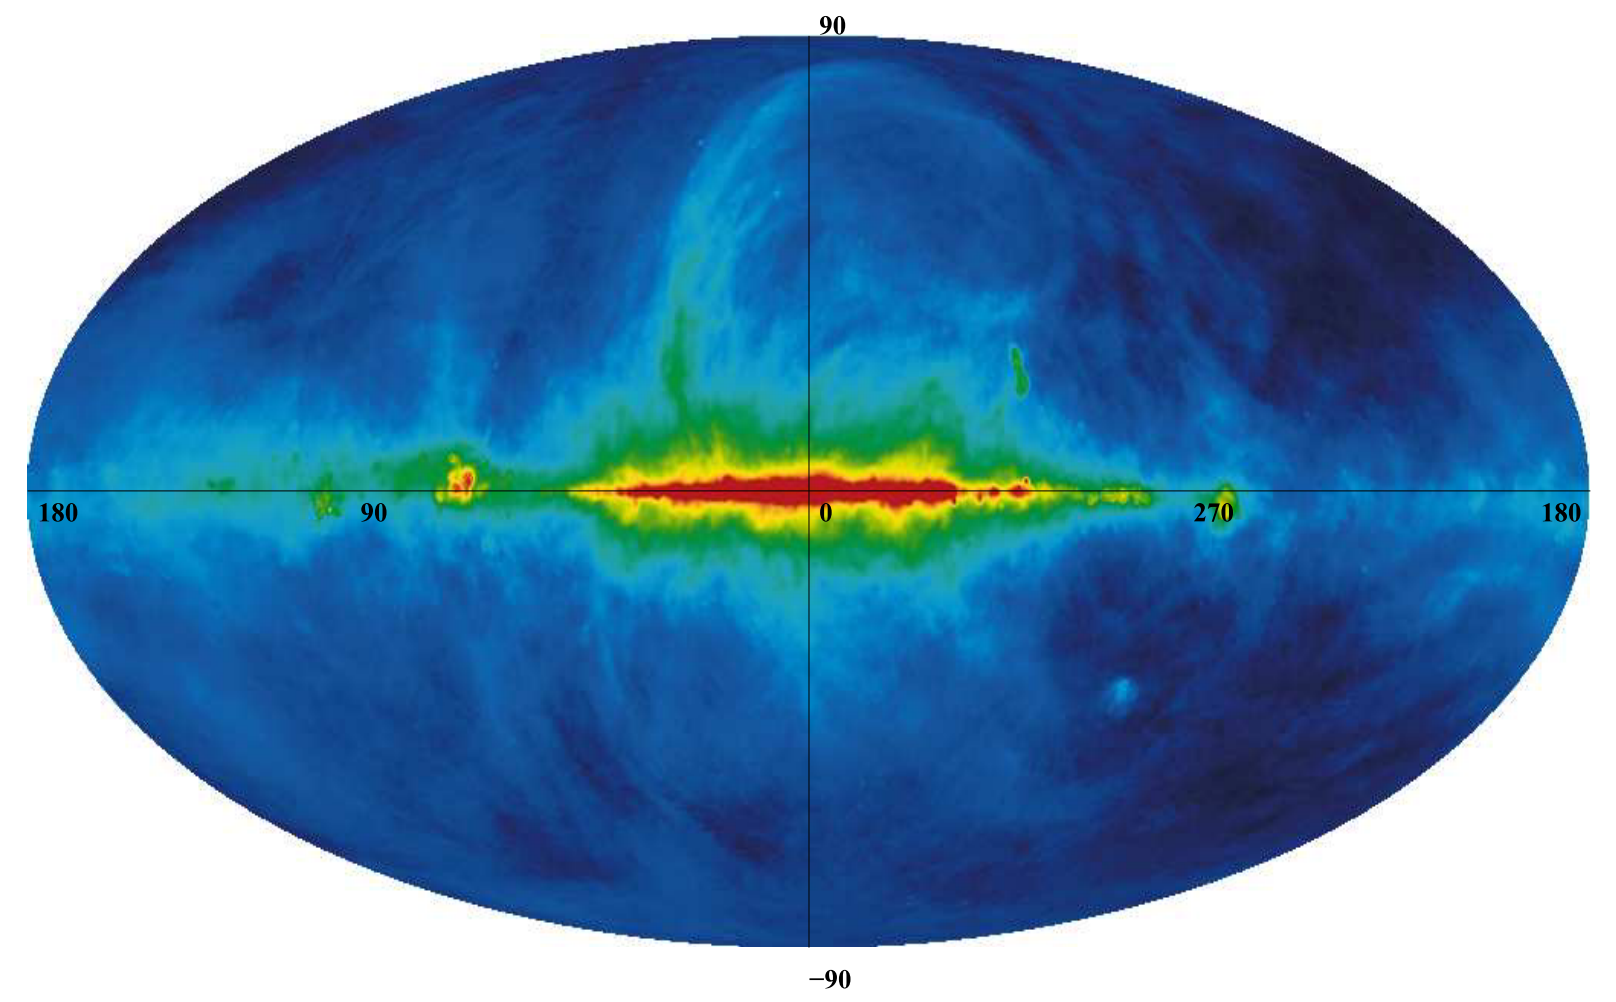
\includegraphics[width=12cm]{figures/Haslam408.png}
    \caption{\footnotesize{The synchrotron emission at $408\,{\rm MHz}$ across the entire sky in Galactic coordinates. As expected the emission is concentrated along the Galactic plane. The noticeable feature known as Loop I is clearly arching up from $\ell=55^\circ$ towards the North Galactic Pole. This figure is adapted from Haslam et al. (1981). Figure taken from Newton-McGee (2009).}}
    \label{fig:haslam408}
\end{figure}

{\noindent}\textbf{Cosmic rays} (i.e., high energy nuclei and electrons) are an important component of the ISM along with magnetic fields and interstellar gas. While the origin of cosmic rays is still not comprehensively understood, it is believed that the electrons with an energy approaching $100-1000\,{\rm TeV}$ have been accelerated in SNRs, suggesting this is one mechanism for the primary formation of cosmic rays.

{\noindent}Magnetic fields accelerate these charged particles via the \textbf{Lorentz force}. The acceleration is given by

\begin{align*}
    \frac{{\rm d}}{{\rm d}\tau}(m\gamma v) = q\left(\frac{\vec{v}}{c}\times\vec{B}\right) ~ [{\rm N}]
\end{align*}

{\noindent}where $m$ is the mass of the particle with charge $q$, $\tau$ is the retarded time, the Lorentz factor  $\gamma=(1 v^2/c^2)^{-1/2}$, and $\vec{B}$ is the magnetic field. The trajectory of the particle is \textit{helical}, with a \textbf{gyration frequency} $\omega_B$ and \textbf{pitch angle} $\theta$ (where $\theta=90^\circ$ for a circular orbit, and $\theta=0^\circ$ for a particle trajectory parallel to $\vec{B}$).

\begin{figure}[h]
    \floatbox[{\capbeside\thisfloatsetup{capbesideposition={right,top},capbesidewidth=4cm}}]{figure}[\FBwidth]
    {\caption{\footnotesize{\\The trajectory of a relativistic electron spiraling in a magnetic field B with a pitch angle $\theta$. The electric field $E$ is polarized parallel to the orbital plane. The synchrotron emission is emitted in a highly beamed cone. This figure is adapted from Kraus (1986). Figure taken from Newton-McGee (2009).}}
    \label{fig:synchrotrondiagram}}
    {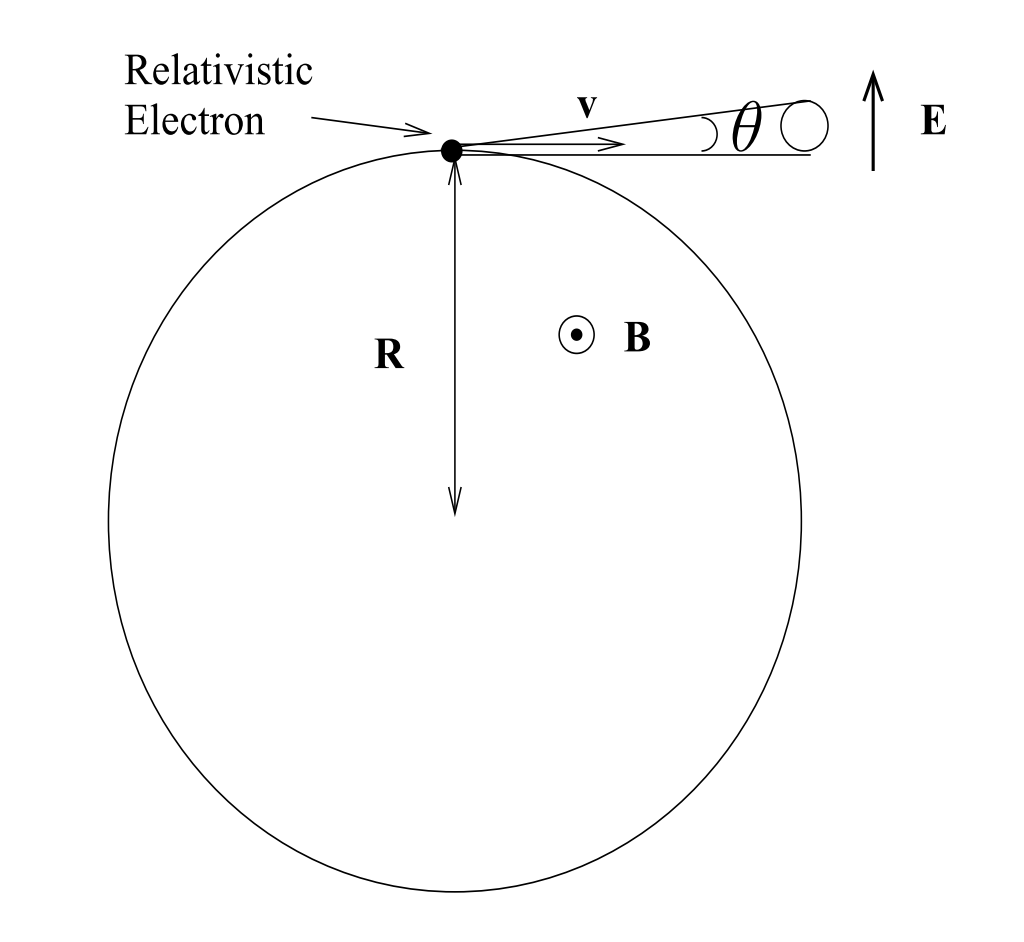
\includegraphics[width=6cm]{figures/SynchrotronDiagram.png}}
\end{figure}

{\noindent}A charged particle deflected by magnetic fields while moving at relativistic speeds emits synchrotron radiation during this acceleration. The main properties of the synchrotron radiation are the following:

\begin{itemize}
    \item high intensity;
    \item very broad and continuous spectral range from infrared up to the hard x-ray region;
    \item natural narrow angular collimation;
    \item high degree of polarization;
    \item pulsed time structure.
\end{itemize}

The graphical representation of synchrotron radiation, depicted in Figure \ref{fig:synchrotrondiagram}, shows that the velocity vector of the particle generates the surface of a cone, with the synchrotron emission beamed within the surface of the cone, at an angle of:

\begin{align*}
    \theta = \pm \frac{mc^2}{E} ~ [{\rm rad}].
\end{align*}

{\noindent}On the surface of the cone the radiation is $100\%$ linearly polarized with its electric field in the direction $-\vec{v}\times\vec{B}$, where $v$ is the direction of propagation of the electron. The degree of linear polarization, called the polarization fraction $p$, is independent of frequency and depends on the spectral index of the cosmic ray electrons:

\begin{align*}
    p(\alpha) = \frac{3-3\alpha}{5-3\alpha} ~ [{\rm dimensionless}].
\end{align*}

{\noindent}In order to understand the angular and spectral distribution of the emitted radiation of synchrotron radiation, let us remind ourselves of the emission from a classical electron moving at a speed $v$ much lower than the speed of light ($v\ll c$). In this case the emitted pattern is similar to that of an oscillating dipole with its maximum of intensity in the direction perpendicular to the acceleration and does not depend on the electron speed. For a relativistic effect, when the speed of the emitting electrons increases to relativistic values ($v\approx c$) the radiation pattern is compressed into a narrow cone in the direction of motion, resulting into an emission tangential to the particle orbit. The vertical half-opening angle $\theta$ is given by

\begin{align*}
    \theta \approx \frac{mc^2}{E} \approx \frac{1}{\gamma} ~ [{\rm rad}].
\end{align*}

{\noindent}See Figure \ref{fig:synchrotronorbits}.

\begin{figure}[h]
    \centering
    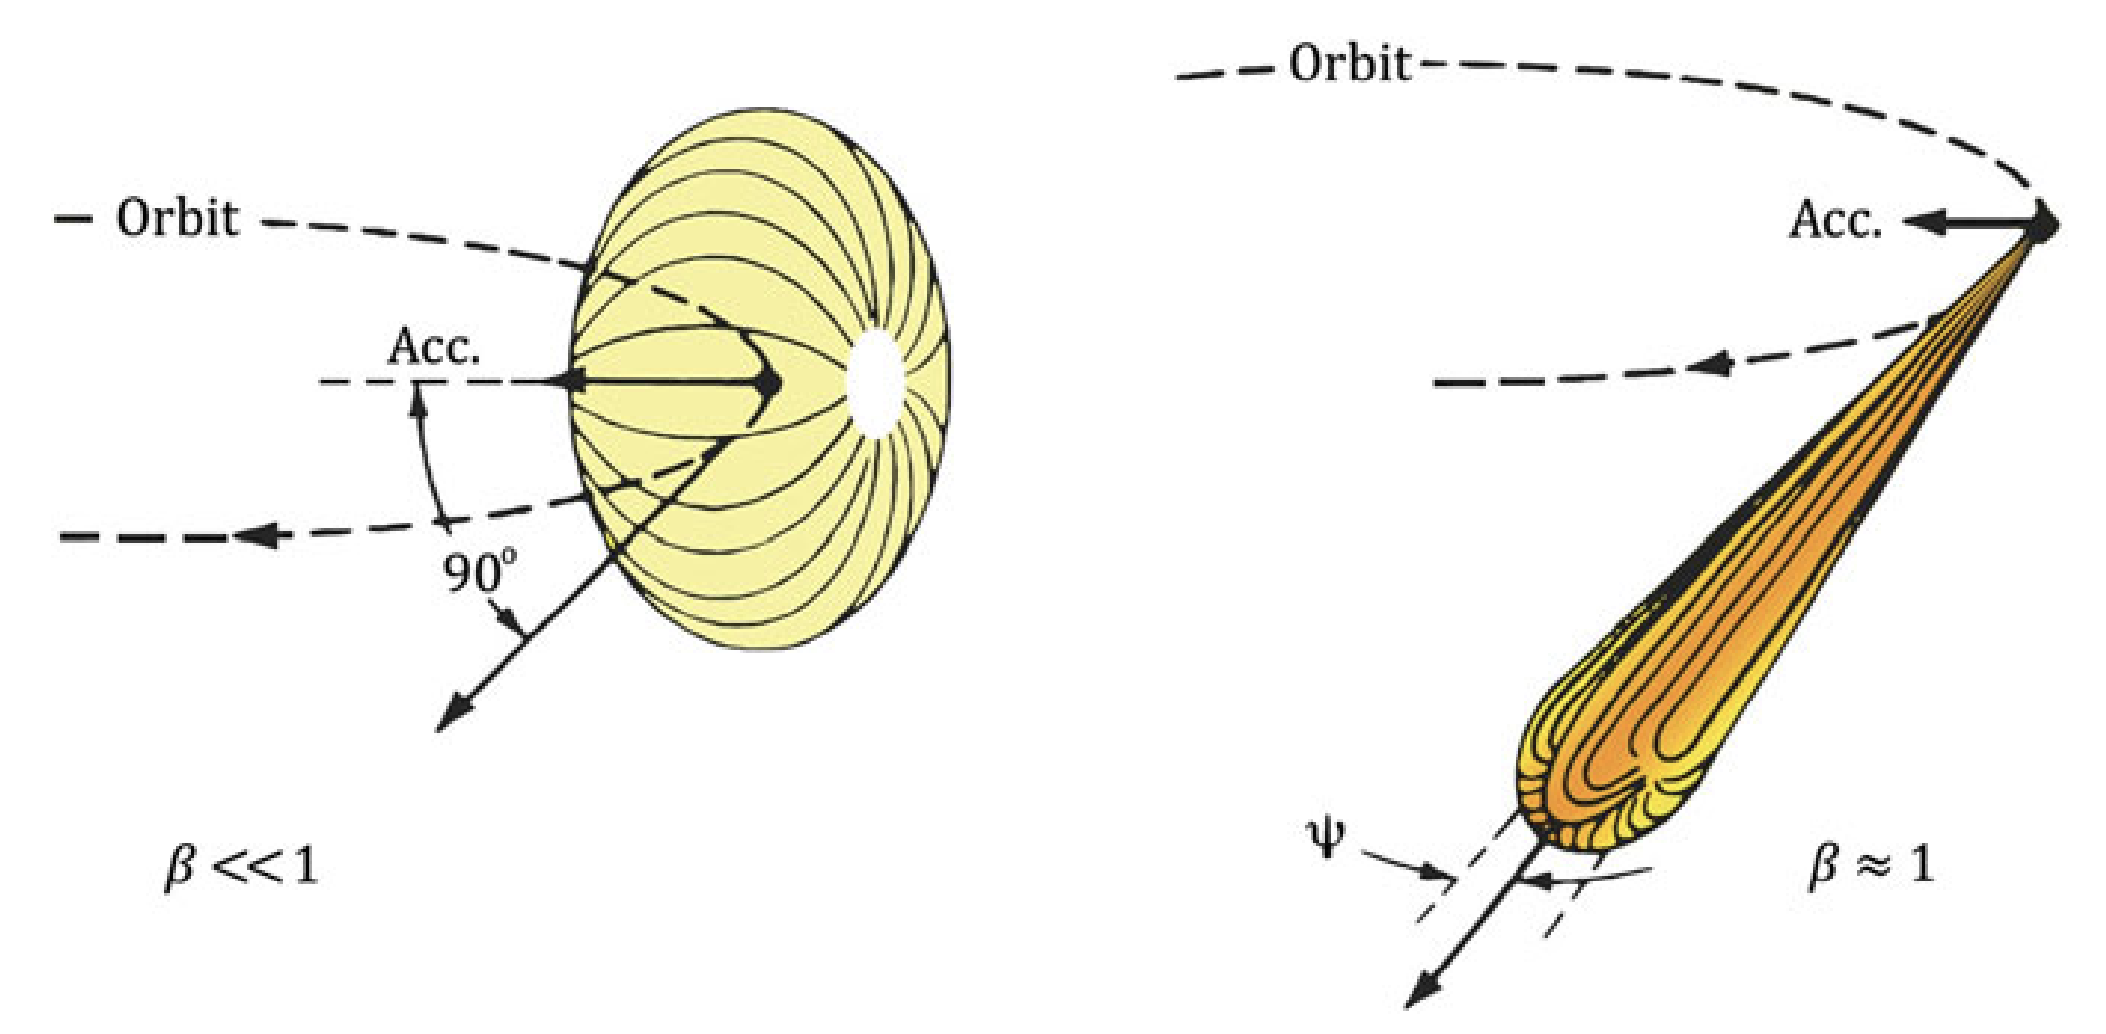
\includegraphics[width=12cm]{figures/SynchrotronOrbits.png}
    \caption{\footnotesize{Qualitative radiation patterns related to charged particles moving in a circular orbit. The dipole pattern is achieved for slow particles when $v/c\ll1$ (left); this is distorted into a narrow cone when $v/c\approx1$ (right). Figure taken from Mobilio et al. (2015).}}
    \label{fig:synchrotronorbits}
\end{figure}

{\noindent}The radiated power from the accelerating charge is given (in cgs units) by

\begin{align*}
    P = \frac{2}{3}\frac{q^4}{m^2c^5} (\gamma\nu)^2 (B\sin\theta)^2 = 2.37\times10^{-15} \left(\frac{E}{{\rm erg}}\right)^2 \left(\frac{B\sin\theta}{\mu{\rm G}}\right)^2 ~ [{\rm erg\,s^{-1}}]
\end{align*}

{\noindent}where the final equality is given for electrons in particular, since the dependence on the mass-to-charge ratio means that electrons are by several orders of magnitude dominant over protons or ions in generating synchrotron radiation. The synchrotron power peaks at the \textbf{characteristic frequency} (in Hz) of

\begin{align*}
    \nu_c = \frac{3}{4\pi}\frac{q}{mc}\gamma^2(B\sin\theta) = 6.26\times10^3 \left(\frac{E}{{\rm erg}}\right)^2 \left(\frac{B\sin\theta}{\mu{\rm G}}\right) ~ [{\rm Hz}].
\end{align*}

{\noindent}This equation tells us that for radio observations (frequencies at or above tens of ${\rm MHz}$) and with typical magnetic field strengths of order $\mu{\rm G}$, the observed population of electrons have $\gamma\gg1$. The radiation is thus highly beamed (width $\sim\gamma^{-1}$) in the direction of the velocity vector. The population of electrons has a power-law energy distribution given by

\begin{align*}
    n(\gamma){\rm d}\gamma = n_0\gamma^{-p}{\rm d}\gamma ~ [{\rm eV^{-1}}]
\end{align*}

{\noindent}where a typical value for the power law index is $p\approx2.5$. The resulting synchrotron luminosity is thus also a power law,

\begin{align*}
    L_\nu \propto \nu^{-(p-1)/2}\equiv \nu^{-\alpha} ~ [{\rm erg\,s^{-1}}]
\end{align*}

{\noindent}with a typical spectral index $\alpha=0.75$ for $p=2.5$. The particles lose energy due to the power emitted with a characteristic timescale of

\begin{align*}
    \tau_{\rm syn} = \frac{\gamma}{{\rm d}\gamma/{\rm d}\tau} = 4\pi\frac{mc}{\sigma_T}\gamma^{-1}(B\sin\theta)^{-2} ~ [{\rm yr}]
\end{align*}

{\noindent}where the \textbf{Thomson cross-section} $\sigma_T=8\pi q^4/3m^2c^4$. Since $\tau_{\rm syn}$ is shorter for more energetic electrons (higher $\gamma$) the power law in the number density $n(\gamma){\rm d}\gamma$ steepens with time (often corresponding to distance from the site of cosmic ray acceleration), therefore increasing the value of $\alpha$. This is referred to as \textbf{synchrotron aging}. Substituting for the characteristic synchrotron frequency $\nu_c$, we can see that

\begin{align*}
    \left(\frac{\tau_{\rm syn}}{{\rm yr}}\right) = 1.06\times10^9 \left(\frac{B\sin\theta}{\mu{\rm G}}\right)^{-1.5} \left(\frac{\nu_c}{{\rm GHz}}\right)^{-0.5}.
\end{align*}

{\noindent}The spectrum of synchrotron radiation must be related to the detailed variation of the electric field as seen by an observer. Because of beaming effects the emitted radiation fields appear to be concentrated in a narrow set of directions about the particle's velocity. The observer will see a pulse of radiation confined to a time interval much smaller than the gyration period. The spectrum will thus be spread over a much broader region than one of order $\omega_B/2\pi$. This is an essential feature of synchrotron radiation.

{\noindent}Non-thermal cosmic radio emission was first thought to originate in stellar atmospheres (the \textbf{radio star hypothesis}). This hypothesis seemed quite reasonable at first glance in view of the existence of quite intense sporadic radio emission from the Sun. It is easy to see, however, that to explain the observed data, these hypothetical radio stars would need to possess extremely unusual properties. The discovery of a quasi-spherical component of the general galactic radio emission imposed severe demands on the radio star hypothesis. For instance, it became clear in this connection that sources of non-thermal galactic radio emission were distributed principally in the galactic halo, the discovery of which had been made only a short time before. Nevertheless, the radio star hypothesis was still not abandoned. If, on the other hand, we equate the general galactic radio emission with synchrotron radiation we then obtain completely probable and useful estimates of the intensity of interstellar fields and the concentration of relativistic electrons. Such estimates are also encouraging in the case of discrete sources. The radio star hypothesis was thus abandoned as early as the beginning of 1953 and the synchrotron character of the major part of non-thermal cosmic radio emission was accepted. 

% --------------------------------------------------------------
%               5. 
% --------------------------------------------------------------

\newpage
\subsection{Question 5}

What are ``forbidden lines'' of atomic spectra? In what conditions are they observationally important? In what conditions do they control the temperature of interstellar material?

\subsubsection{Short answer}

Answer.

\subsubsection{Additional context}

{\noindent}\textbf{Brief overview of atomic structure:} Atoms consist of three subatomic particles: protons, neutrons, and electrons. A proton has a positive charge and a neutron has no charge. Both protons and neutrons are found in the densely packed, positively charged nucleus. The nucleus contains essentially all of the mass of the atom. Electrons carry a negative charge and are found in electron shells surrounding the nucleus. The mass of the electron is considered to be negligible.

{\noindent}All atoms have an atomic number, $Z$, and a mass number, $A$. The atomic number, $Z$, represents its number of protons and its mass number, $A$, represents its number of protons plus its number of neutrons. All atoms of a particular element will have the same atomic number, however they may differ in their number of neutrons and electrons. Two atoms with the same atomic number but different mass numbers (different numbers of neutrons) are referred to as \textbf{isotopes}. The average atomic mass found on the periodic table represents a weighted average of the naturally occurring isotopes for a particular element. Atoms with unequal numbers of protons and electrons produce charged atoms or \textbf{ions}.

{\noindent}Electrons within an atom are found in particular \textbf{orbitals}. An atomic orbital is a mathematical function that describes the wave-like behavior of either one electron or a pair of electrons in an atom. This function can be used to calculate the probability of finding any electron of an atom in any specific region around the atom's nucleus. The term atomic orbital may also refer to the physical region or space where the electron can be calculated to be present, as defined by the particular mathematical form of the orbital. 

{\noindent}Electrons within an atom can be assessed according to the shell, subshell, and orbital to which they are assigned. These assessments are based on the quantum mechanical model. \textbf{Shells} are numbered as $n=1$, $2$, $3$, $4$, etc. and increase in size and energy as they get further away from the nucleus. Shells can be subdivided into subshells.

{\noindent}The maximum number of \textbf{subshells} is equivalent to the shell number. For example, when $n=1$ (first shell), only one subshell is possible and when $n=2$ (second shell), two subshells are possible. There are four different types of subshells. These various types of subshells are denoted by the letters $s$, $p$, $d$, and $f$. Each subshell has a maximum number of electrons which it can hold: $s$: $2$ electrons, $p$: $6$ electrons, $d$: $10$ electrons, and $f$: $14$ electrons. The $s$ subshell is the lowest energy subshell and the $f$ subshell is the highest energy subshell. As was mentioned previously, the shell number is equal to the possible number of subshells. Thus, when $n=1$, the only subshell possible is the $1s$ subshell. When $n=2$, two subshells are possible: the $2s$ and $2p$. When $n=3$, three subshells are possible: the $3s$, $3p$, and $3d$. This means that in the first shell only two electrons are possible and they would be found in the $1s$ ($2$ electrons) subshell. In the second shell, $8$ electrons are possible and would be found in the $2s$ ($2$ electrons) and the $2p$ ($6$ electrons) subshells.

{\noindent}Each subshell is further divided into \textbf{orbitals}. An orbital is defined as a region of space in which an electron can be found. \textit{Only two electrons are possible per orbital}. Thus, the $s$ subshell may contain only one orbital and the $p$ subshell may contain three orbitals. Each orbital has its own distinct shape. An $s$ orbital found in an $s$ subshell is spherical, $p$ orbitals found in $p$ subshells are two-lobed, and $d$ orbitals found in $d$ subshells are four-lobed. Since there are three possible orbitals per $p$ subshell, each orbital adopts its own orientation. The $p_x$ orbital lies along the $x$ axis, the $p_y$ orbital lies along the $y$ axis, and the $p_z$ orbital lies along the $z$ axis.

\begin{figure}[t]
    \centering
    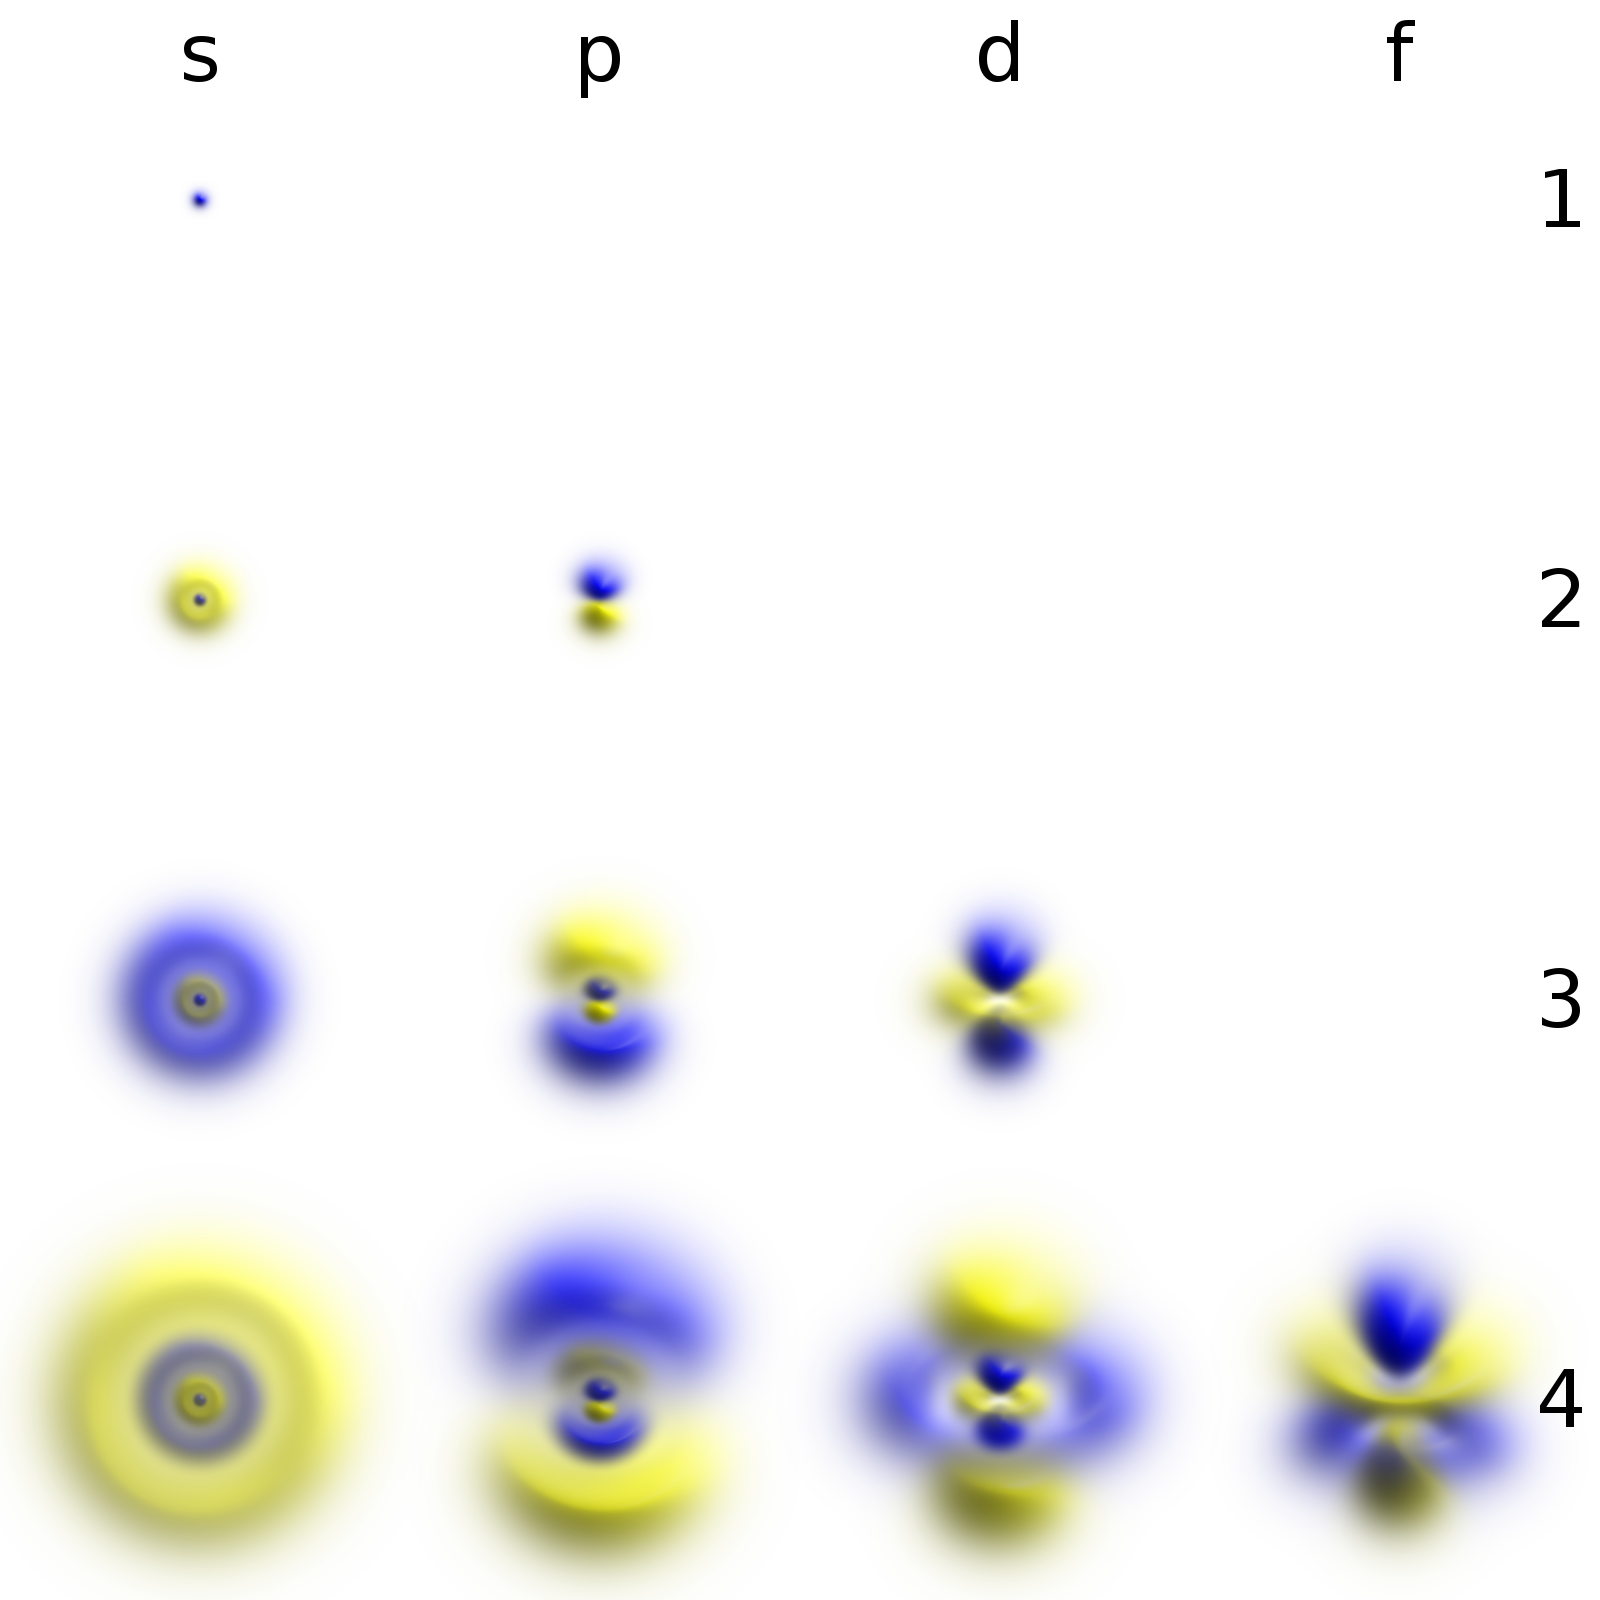
\includegraphics[width=11cm]{figures/orbitals_3D.png}
    \caption{\footnotesize{3D views of some hydrogen-like atomic orbitals. Figure taken from Wikipedia.}}
    \label{fig:orbitals3D}
\end{figure}

{\noindent}When writing electron configurations for atoms, the shorthand symbol for a subshell followed by a super-scripted number which represents the number of electrons in that subshell is used. For example, a Carbon atom with $6$ electrons would have the electron configuration: $1s^22s^22p^2$. A possible arrangement within the $2p$ subshell would be to find one of the electrons in the $2p_x$ orbital and the second electron in the $2p_y$ orbital. 

{\noindent}Figure \ref{fig:orbitals3D} shows hydrogen-like atomic structure for $s$, $p$, $d$, and $f$ orbitals.

{\noindent}\textbf{Selection rules for radiative transitions:} Some energy levels are connected by strong radiative transitions; in other cases, radiative transitions between the levels may be extremely slow. The strong transitions always satisfy what are referred to as the \textbf{selection rules for electric dipole transitions}. Here, we summarize the selection rules for the strong electric dipole transitions, and we also give the selection rules for \textbf{inter-system} and \textbf{forbidden transitions} that do not satisfy the electric dipole selection rules but nevertheless are strong enough to be astrophysically important. We will use the ion NII as an example; the first nine energy levels of NII are shown in Figure \ref{fig:NIIlevels}.

\begin{figure}[t]
    \centering
    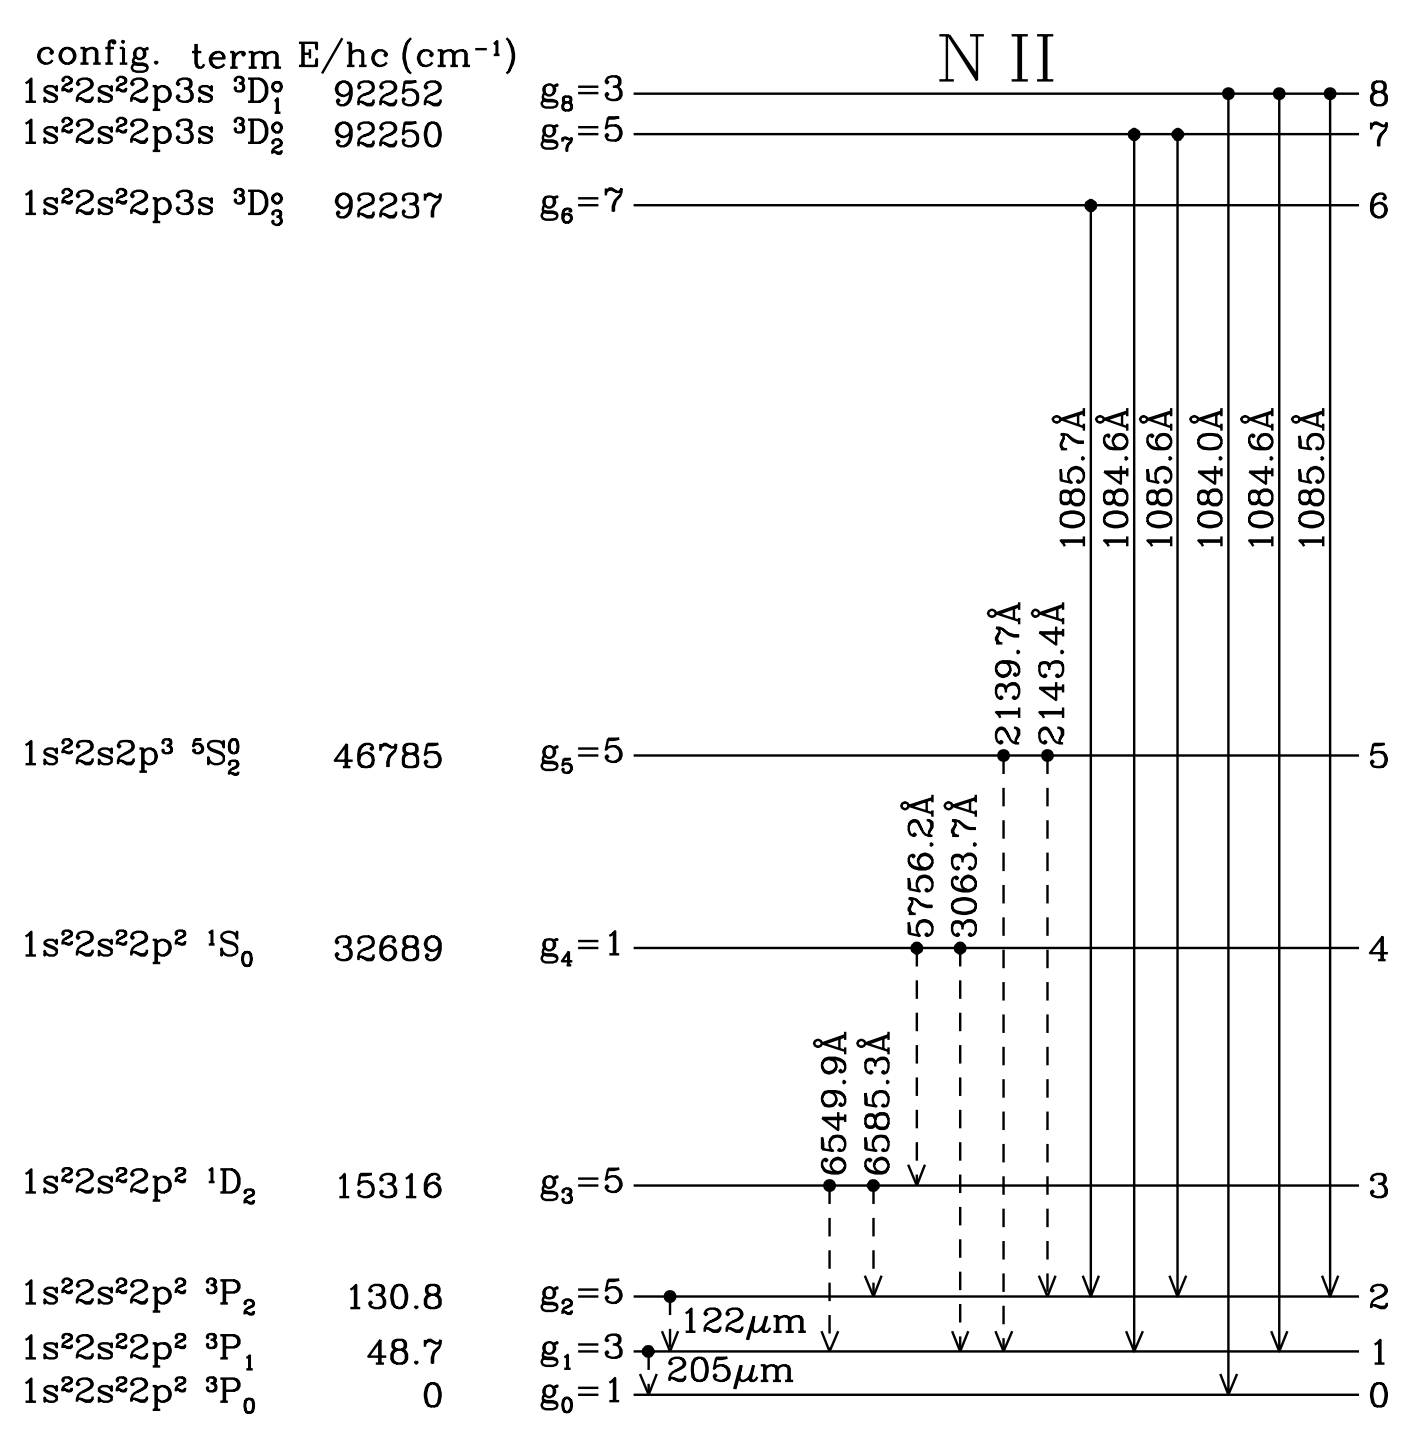
\includegraphics[width=14cm]{figures/NII_levels.png}
    \caption{\footnotesize{First nine energy levels of NII. Forbidden transitions are indicated by broken lines, and allowed transitions by solid lines; forbidden decays are not shown from levels that have permitted decay channels. Fine-structure splitting is not to scale. Hyperfine splitting is not shown. Figure taken from Draine (2015).}}
    \label{fig:NIIlevels}
\end{figure}

{\noindent}\textbf{Allowed: Electric dipole transitions:} The strongest transitions are electric dipole transitions. These are transitions satisfying the following selection rules:

\begin{enumerate}
    \item Parity must change.
    \item $\Delta L = 0, \pm1$.
    \item $\Delta J = 0, \pm1$, but $\Delta J = 0\rightarrow0$ is forbidden.
    \item Only one single-electron wave function $n\ell$ changes, with $\Delta\ell=\pm1$.
    \item $\Delta S=0$: Spin does not change.
\end{enumerate}

{\noindent}An allowed transition is denoted \textit{without} square brackets, for example,

\begin{align*}
    {\rm NII}\,1084.0{\rm \AA}\,^3P_0-^3D_1^o.
\end{align*}

{\noindent}This is a transition between the $\ell=1s^22s^22p^2\,3P_0$ and $u=1s^22s^22p3s\,^3D_1^o$ levels of NII, with a wavelength $\lambda_{u\ell}=1084.0$\,\AA. The transition has $A_{u\ell}=2.18\times10^8\,{s^{-1}}$. This decay is very fast -- the lifetime of the $^3D_1^o$ level against this decay is only $1/A_{u\ell}=4.6\,{\rm ns}$!

{\noindent}\textbf{Spin-Forbidden or inter-system transitions:} These are transitions that fulfill the electric dipole selection rules $1$ to $4$ but have $\Delta S\neq0$. These transitions are considerably weaker than allowed transitions. Such transitions are sometimes referred to as \textbf{semi-forbidden}, or \textbf{inter-combination}, or \textbf{inter-system transitions}; the latter is the terminology that we will use. An inter-system transition is denoted with a single right bracket -- for example,

\begin{align*}
    {\rm NII]}\,2143.4{\rm \AA}\,^3P_2-^5S_2^o.
\end{align*}

{\noindent}This is a transition between the $\ell=1s^22s^22p^2\,3P_2$ and $u=1s^22s2p^3\,^5S_2^o$ levels of NII, with a wavelength $\lambda_{u\ell}=2143.4$\,\AA\,and $A_{u\ell}=1.27\times10^2\,{\rm s^{-1}}$.

{\noindent}\textbf{Forbidden transitions:} Forbidden transitions are those that fail to fulfill at least one of the selection rules $1$ to $4$. The transition probabilities vary widely, depending on the values of the electric quadrupole or magnetic dipole matrix elements between the upper and lower states. A forbidden transition is denoted with two square brackets -- for example,

\begin{align*}
    {\rm [NII]}\,6549.9{\rm \AA}\,^3P_1-^1D_2^o.
\end{align*}

{\noindent}This is a transition between the $\ell=1s^22s^22p^2\,3P_1$ and $u=1s^22s^22p^2\,^1D_2^o$ levels of NII, with a wavelength $\lambda_{u\ell}=6549.9$\,\AA\,and $A_{u\ell}=9.20\times10^{-4}\,{\rm s^{-1}}$. This fails rule $1$ (parity is unchanged) and it fails rule $4$ (single electron wave functions are unchanged). This is an example of a \textbf{magnetic dipole transition}.

{\noindent}Another example of a forbidden transition is the \textbf{electric quadrupole transition}

\begin{align*}
    {\rm [NII]}\,5756.2{\rm \AA}\,^1D_2-^1S_0^o.
\end{align*}

{\noindent}This is a transition between the $\ell=1s^22s^22p^2\,1D_2$ and $u=1s^22s^22p^2\,^1S_0^o$ levels of NII, with a wavelength $\lambda_{u\ell}=5756.2$\,\AA\,and $A_{u\ell}=1.17\,{\rm s^{-1}}$. This fails rules $1$ (parity is unchanged) and $4$ (single electron wave functions are unchanged) and it fails rules $2$ and $3$ ($\Delta L=-2$ and $\Delta J=-2$), yet its transition probability is three orders of magnitude larger than the magnetic dipole transition [NII]\,$6549.9$\AA!

{\noindent}We see then that there is a hierarchy in the transition probabilities: very roughly speaking, inter-system lines are $\sim10^6$ times weaker than permitted transitions, and forbidden lines are $\sim10^2-10^6$ times weaker than inter-system transitions.

{\noindent}Despite being very ``weak,'' forbidden transitions are important in astrophysics for the simple reason that every atom and ion has excited states that can only decay via forbidden transitions. At high densities, such excited states would be depopulated by collisions, but at the very low densities of interstellar space, collisions are sufficiently infrequent that there is time for forbidden radiative transitions to take place.

\subsubsection{Follow-up Questions}

\begin{itemize}
    \item What are some common examples of forbidden lines?
    \item When do you get forbidden line absorption?
    \item What kind of radiation can be absorbed by forbidden line absorption?
    \item Can we observe any forbidden lines on Earth?
    \item What is the lifetime of the 21 cm line?
    \item At what redshifts do CMB photons get absorbed by 21 cm transitions?
    \item At what redshifts do you get neutral hydrogen?
    \item How would you estimate the lifetime from the maximum density where the line isn't washed out?
    \item Collisions happen much more frequently; why is the 21 cm line still visible?
    \item Why does forbidden line emission cool the gas?
    \item Why are they \textit{so good} at cooling the gas?
\end{itemize}

% --------------------------------------------------------------
%               6. 
% --------------------------------------------------------------

\newpage
\subsection{Question 6}

What is a polytropic equation of state? Give examples of objects for which this is a very good approximation, and explain why it is.

\subsubsection{Short answer}

Answer.

\subsubsection{Additional context}

{\noindent}\textbf{Eulerian description}: For gaseous, non-rotating, single stars without strong magnetic fields, the only forces acting on a mass element come from pressure and gravity. This results in a spherically symmetric configuration. All functions will then be constant on concentric spheres, and we need only one spatial variable to describe them. It seems natural to use the distance r from the stellar centre as the spatial coordinate, which varies from r D 0 at the centre to the total radius r D R at the surface of the star. In addition, the evolution in time t requires a dependence of all functions on t: If we thus take r and t as independent variables, we have a typical ``Eulerian'' treatment in the sense of classical hydrodynamics. Then all other variables are considered to depend on these two, for example, the density $\rho=\rho(r,t)$.

{\noindent}\textbf{Lagrangian description}: It will turn out that, in the spherically symmetric case, it is often more useful to take a ``Lagrangian'' coordinate instead of r (i.e., one which is connected to the mass elements). The spatial coordinate of a given mass element then does not vary in time. We choose for this coordinate the above defined $m$: to any mass element, the value $m$ (which is the mass contained in a concentric sphere at a given moment $t_0$) is assigned once and for all.

{\noindent}The new independent variables are then $m$ and $t$; and all other variables are considered to depend on them; for example, $\rho=\rho(m,t)$. This also includes the radial distance $r$ of our mass element from the centre, which is now described by the function $r=r(m,t)$. Since there is certainly no singularity of $\rho$ at the centre, we have here $m=0$, while the star's total mass $m=M$ is reached at the surface (i.e., where $r=R$). This already shows one advantage of the new description for the (normal) case of stars with constant total mass: while the radius $R$ varies strongly in time, the star always extends over the same interval of the independent variable $m:0\leq m \leq M$. Although real stars do lose mass, for example, by stellar winds or due to gravitational interaction in binary systems, over short timescales the assumption of constant mass is justified nevertheless. In any case, the range of $m$ never changes by more than a factor of a few.

{\noindent}As just indicated, there will certainly be no problem concerning a unique one-to-one transformation between the two coordinates $r$ and $m$: We then easily find the connection between the partial derivatives in the two cases from well-known formulae. For any function depending on two variables, one of which is substituted by a new one ($r,t\rightarrow m,t$), the partial derivatives with respect to the new variables are given by

\begin{align*}
    \frac{\partial}{\partial m} &= \frac{\partial}{\partial r} \cdot \frac{\partial r}{\partial m} \\
    \left(\frac{\partial}{\partial t}\right)_m &= \frac{\partial}{\partial r}\cdot \left(\frac{\partial r}{\partial t}\right)_m + \left(\frac{\partial}{\partial t}\right)_r.
\end{align*}

{\noindent}Subscripts indicate which of the spatial variables ($m$ or $r$) is considered constant. The second of these equations reveals the main reason for the choice of the Lagrangian description. Its left-hand side gives the so-called \textbf{substantial time derivative} of hydrodynamics. It describes the change of a function in time when following a given mass element (e.g., the change of a physical property of this mass element). The conservation laws for time-dependent spherical stars give very simple equations only in terms of this substantial time derivative. In terms of a local time derivative, $(\partial/\partial t)_r$, the description would become much more complicated since the ``convective'' terms with the velocity $(\partial r/\partial t)_m$ would appear explicitly.

{\noindent}Let us apply the first of these to $m$. We know that $m$ varies with $r$ as

\begin{align*}
    \frac{\partial m}{\partial r} = 4\pi r^2 \rho.
\end{align*}

{\noindent}Taking the partial derivative $\partial/\partial m$, we obtain

\begin{align*}
    \frac{\partial}{\partial m} \left(\partial m\right) &= \frac{\partial}{\partial m} \left(4\pi r^2 \rho\right) \partial r \\
    1& = \frac{\partial r}{\partial m} \left(4\pi r^2 \rho\right) \\
    \frac{\partial r}{\partial m} &= \frac{1}{4\pi r^2 \rho}.
\end{align*}

{\noindent}This is a differential equation describing the spatial behaviour of the function $r(m,t)$. It replaces $\partial m/\partial r=4\pi r^2\rho$ in the Lagrangian description. Introducing this differential equation into the partial differential equation we just found for $\partial/\partial m$, we find the general recipe for the transformation between the two operators:

\begin{align*}
    \frac{\partial}{\partial m} = \frac{1}{4\pi r^2\rho} \frac{\partial}{\partial r}.
\end{align*}

{\noindent}In the deep interiors of stars the gases are fully ionized (i.e., for each hydrogen nucleus there also exists a free electron, while for each helium nucleus there are two free electrons). We therefore have a mixture of two gases, that of the nuclei (which in itself can consist of more than one component) and that of the free electrons. The mixture can be treated similarly to a one-component gas, if all single components obey the ideal gas law.

{\noindent}Let's consider a mixture of fully ionized nuclei. The chemical composition can be described by specifying all $X_i$ ; the weight fractions of nuclei of type $i$ which have molecular weight $\mu_i$ and charge number $Z_i$. If we have $n_i$ nuclei per volume and a ``partial density'' $\rho_i$, then $X_i=\rho_i/\rho$ and

\begin{align*}
    n_i = \frac{\rho_i}{\mu_im_{\rm H}} = \frac{\rho}{m_{\rm H}} \frac{X_i}{\rho_i}.
\end{align*}

{\noindent}By $L_r$ we define the net energy per second passing outward through a sphere of radius $r$. The function $L_r$ is zero at $r=0$, since there can be no infinite energy source at the centre, while $L_r$ reaches the total luminosity $L$ of the star at the surface. In between, $L_r$ can be a complicated function, depending on the distribution of the sources and sinks of energy.

{\noindent}The function $L_r$ comprises the energies transported by radiation, conduction, and convection. Not included is a possible energy flux by neutrinos, which normally have negligible interaction with the stellar matter. Also included in $L_r$ are only those fluxes which require a temperature gradient.

{\noindent}Consider a spherical mass shell of radius $r$; thickness ${\rm d}r$; and mass ${\rm d}m$. The energy per second entering the shell at the inner surface is $L_r$, while $L_r+{\rm d}L_r$ is the energy per second leaving it through the outer surface. The surplus power ${\rm d}L_r$ can be provided by nuclear reactions, by cooling, or by compression or expansion of the mass shell.

{\noindent}We first consider a stationary case in which ${\rm d}L_r$ is due to the release of energy from nuclear reactions only. Let $\epsilon$ be the \textbf{nuclear energy produced per gram of stellar material}; then

\begin{align*}
    {\rm d}L_r &= 4\pi r^2\rho\epsilon{\rm d}r = \epsilon {\rm d}m \\
    \frac{{\rm d}L_r}{{\rm d}m} &= \epsilon ~ [{\rm eV\,g^{-1}}].
\end{align*}

{\noindent}In general $\epsilon$ depends on the temperature and density, and on the abundance of the different nuclear species that react.

{\noindent}Let us denote the types of reacting particles, $X$ and $a$, by indices $j$ and $k$ respectively. Suppose there is one particle of type $j$ moving with a velocity $v$ relative to all particles of type $k$. Its cross section $\sigma$ for reactions with $k$ sweeps over a volume $\sigma v$ per second. The number of reactions per second will then be $n_k \sigma v$ if there are $n_k$ particles of type $k$ per unit volume. For $n_j$ particles per unit volume the total number of reactions per units of volume and time is

\begin{align*}
    \tilde{r}_{jk} = n_jn_k\sigma v.
\end{align*}

{\noindent}This product may also be interpreted by saying that $n_jn_k$ is the number of pairs of possible reaction partners, and $\sigma v$ gives the reaction probability per pair and second. This indicates what we have to do in the case of reactions between identical particles ($j=k$). Then the number of pairs that are possible reaction partners is $n_j(n_j-1)/2\approx n_j^2/2$ for large particle numbers. This has to replace the product $n_jn_k$ so that we can generally write

\begin{align*}
    \tilde{r}_{jk} = \frac{1}{1+\delta_{jk}}n_jn_k\sigma v
\end{align*}

{\noindent}\textbf{The full set of equations}: Collecting the basic differential equations for a spherically symmetric star in hydrostatic equilibrium, we obtain a full set of differential equations that describe stellar evolution:

\begin{equation*}
\boxed{
    \begin{aligned}
        \frac{\partial r}{\partial m} &= \frac{1}{4\pi r^2\rho} \\
        \frac{\partial P}{\partial r} &= -\frac{GM_r}{4\pi r^4} \\
        \frac{\partial L}{\partial m} &= \epsilon_n-\epsilon_\nu-c_P \frac{\partial T}{\partial t} + \frac{\delta}{\rho}\frac{\partial P}{\partial t} \\
        \frac{\partial T}{\partial m} &= -\frac{GM_rT}{4\pi r^4P}\nabla \\
        \frac{\partial X_i}{\partial t} &= \frac{m_i}{\rho} \left(\sum_jj_{ji} - \sum_kr_{ik}\right), ~~~ i=1,...,I.
    \end{aligned}
}
\end{equation*}

{\noindent}The second equation has an additional term $-\partial^2r/\partial t^2(4\pi r^2)^{-1}$ in case the assumption of hydrostatic equilibrium is not fulfilled. In the last equation, we have a set of $I$ equations (one of which may be replaced by the normalization $\sum_iX_i=1$) for the change of mass fractions $X_i$ of the relevant nuclei $i=1,..,I$ having masses $m_i$. In the third equation, $\delta\equiv-(\partial\ln\rho/\partial\ln T)_P$, and in the second last equation $\nabla\equiv{\rm d}\ln T/{\rm d}\ln P$. If the energy transport is due to radiation (and conduction), then $\nabla$ has to be replaced by $\nabla_{\rm rad}$ given by 

\begin{align*}
    \nabla_{\rm rad} = \frac{3}{16\pi acG}\frac{\kappa LP}{mT^4} ~ [{\rm K\,P^{-1}}].
\end{align*}

{\noindent}If the energy is carried by convection, then $\nabla$ has to be replaced by a value obtained from a proper theory of convection; this may be $\nabla_{\rm ad}$ in the deep interior given by 

\begin{align*}
    \nabla_{\rm ad} = \left(1-\frac{1}{\gamma}\right) \frac{\mu m_{\rm H}}{k}\frac{GM_r}{r^2} ~ [{\rm K\,m^{-1}}],
\end{align*}

{\noindent}or one obtained from a solution of the cubic equation for super-adiabatic convection in the outer layers.

{\noindent}The boxed equations contain functions which describe properties of the stellar material such as $\rho, \epsilon_n, \epsilon_\nu,\kappa,c_P,$ and the reaction rates $r_{ij}$. We shall assume them to be known functions of $P, T$, and the chemical composition described by the functions $X_i(m,t)$ We therefore have an equation of state

\begin{align*}
    \rho = \rho(P,T,X_i) ~ [{\rm g\,cm^{-3}}],
\end{align*}

{\noindent}and equations for the other thermodynamic properties of the stellar matter

\begin{align*}
    c_P &= c_P (P,T,X_i) \\
    \delta &= \delta (P,T,X_i) \\
    \nabla_{\rm ad} &= \nabla_{\rm ad} (P,T,X_i),
\end{align*}

{\noindent}as well as the Rosseland mean of the opacity (including conduction)

\begin{align*}
    \kappa = \kappa (P,T,X_i),
\end{align*}

{\noindent}and the nuclear reaction rates and the energy production and energy loss via neutrinos:

\begin{align*}
    r_{jk} &= r_{jk} (P,T,X_i) \\
    \epsilon_\nu &= \epsilon_\nu (P,T,X_i) \\
    \epsilon_\nu &= \epsilon_\nu (P,T,X_i).
\end{align*}

{\noindent}\textbf{Polytropic equations}: The temperature does not appear explicitly in the first two boxed equations. Under certain circumstances this provides the possibility of separating them from the ``thermo-energetic part'' of the equations. For the following it is convenient to introduce the gravitational potential $\Phi$. We here treat stars in hydrostatic equilibrium, which requires

\begin{align*}
    \frac{{\rm d}P}{{\rm d}r} = - \frac{{\rm d}\Phi}{{\rm d}r} \rho,
\end{align*}

{\noindent}together with Poisson's equation

\begin{align*}
    \frac{1}{r^2}\frac{{\rm d}}{{\rm d}r} \left(r^2\frac{{\rm d}\Phi}{{\rm d}r}\right) = 4\pi G\rho.
\end{align*}

{\noindent}We have replaced the partial derivatives by ordinary ones since only time-independent solutions shall be considered.

{\noindent}In general the temperature appears in these equations if the density is replaced by an equation of state of the form $\rho=\rho(P,T)$. However, if $\rho$ does not depend on $T$ (i.e., $\rho=\rho(P)$), then this relation can be introduced, which become a system of two equations for $P$ and $\Phi$ and can be solved without the other structure equations. An example is the completely degenerate gas of non-relativistic electrons for which $\rho\sim P^{3/5}$.

{\noindent}We shall deal here with similar cases and assume that there exists a simple relation between $P$ and $\rho$ of the form

\begin{align*}
    P = K\rho^\gamma \equiv K\rho^{1+1/n} ~ [{\rm P}],
\end{align*}

{\noindent}where $K$, $\gamma$, and $n$ are constants. A relation of this form is called a \textbf{polytropic equation of state}. $K$ is the \textbf{polytropic constant} and $\gamma$ is the \textbf{polytropic exponent} (which we have to distinguish from the adiabatic exponent $\gamma_{\rm ad}$). One often uses, instead of $\gamma$, the \textbf{polytropic index} $n$, which is defined by

\begin{align*}
    n = \frac{1}{\gamma-1} ~ [{\rm dimensionless}].
\end{align*}

{\noindent}For a completely degenerate gas the equation of state in its limiting cases has the polytropic form as seen above. In the non-relativistic limit we have $\gamma=5/3$, $n=3/2$, while for the relativistic limit $\gamma=4/3$, $n=3$. For such cases, where the equation of state has a polytropic form, the polytropic constant $K$ is fixed and can be calculated from natural constants. There are also examples of the polytropic equation of state where $K$ is a free parameter which is constant within a particular star but can have different values from one star to another.

{\noindent}In a star that is completely convective the temperature gradient (except for that in a region near the surface, which we shall ignore) is given, to a very good approximation, by $\nabla=({\rm d}\ln T/{\rm d}\ln P)_{\rm ad}=\nabla_{ad}$. If radiation pressure can be ignored and the gas is completely ionized, we have $\nabla_{\rm ad}=2/5$. This means that throughout the star $T\sim P^{2/5}$, and for an ideal gas with $\mu={\rm constant}$, $T\sim P/\rho$, and therefore $P\sim\rho^{5/3}$. This again is a polytropic relation with  $\gamma=5/3$, $n=3/2$. But now $K$ is not fixed by natural constants; it is a free parameter in the sense that it can vary from star to star.

{\noindent}The homogeneous gaseous sphere can also be considered a special case of the polytropic relation. Let us write the polytropic equation of state in the form

\begin{align*}
    \rho = K_1P^{1/\gamma} ~ [{\rm g\,cm^{-3}}].
\end{align*}

{\noindent}Then $\gamma=\infty$ (or $n=0$) gives $\rho=K_1={\rm constant}$.

{\noindent}These examples have shown that we can have two reasons for a polytropic relation in a star:
\begin{enumerate}
    \item The equation of state is of the simple form $P=K\rho$ with a fixed value of $K$;
    \item The equation of state contains $T$ (as for an ideal gas), but there is an additional relation between $T$ and $P$ (like the adiabatic condition) that together with the equation of state yields a polytropic relation; then $K$ is a free parameter.
\end{enumerate}

{\noindent}On the other hand, if we assume a polytropic relation for an ideal gas, this is equivalent to adopting a certain relation $T=T(P)$. This means that one fixes the temperature stratification instead of determining it by the thermo-energetic equations of stellar structure. For example, a polytrope with $n=3$ does not necessarily have to consist of relativistic degenerate gases but can also consist of an ideal gas and have $\nabla=1/(n+1)=0.25$.

{\noindent}\textbf{Polytropic stellar models}: With the polytropic relation (independent of whether $K$ is a free parameter or a constant with a fixed value), the equation of hydrostatic equilibrium can be written as

\begin{align*}
    \frac{{\rm d}\Phi}{{\rm d}r} = -\gamma K\rho^{\gamma-2} \frac{{\rm d}\rho}{{\rm d}r}.
\end{align*}

{\noindent}If $\gamma\neq1$ (the case $\gamma=1, n=\infty$ corresponding to the isothermal model, this can be integrated:

\begin{align*}
    \rho = \left( \frac{-\Phi}{(n+1)K} \right)^n ~ [{\rm g\,cm^{-3}}],
\end{align*}

{\noindent}where we have made use of $n=1/(\gamma-1)$ and chosen the integration constant to give $\Phi=0$ at the surface ($\rho=0$). Note that in the interior of our model, $\Phi<0$, giving there $\rho>0$. If we introduce this form of $\rho$ into the right-hand side of the Poisson equation, we obtain an ordinary differential equation for $\Phi$:

\begin{align*}
    \frac{{\rm d}^2\Phi}{{\rm d}r^2} + \frac{2}{r}\frac{{\rm d}\Phi}{{\rm d}r} = 4\pi G \left( \frac{-\Phi}{(n+1)K} \right)^n.
\end{align*}

{\noindent}We now define dimensionless variables $z$, $w$ by

\begin{align*}
    z &= Ar ~ [{\rm dimensionless}], ~~~ A^2 = \frac{4\pi G}{(n+1)^nK^n}(-\Phi^c)^{n-1} = \frac{4\pi G}{(n+1)K}\rho_c^{(n-1)/n} ~ [{\rm dimensionless}],\\
    w &= \frac{\Phi}{\Phi_c} = \left(\frac{\rho}{\rho_c}\right)^{1/n} ~ [{\rm dimensionless}],
\end{align*}

{\noindent}where the subscript $c$ refers to the centre and where the relation between $\rho$ and $\Phi$ is taken from $\rho=[-\Phi/(n+1)K]^n$. At the centre ($r=0$) we have $z=0, \Phi=\Phi_c, \rho=\rho_c$, and therefore $w=1$. Then the ordinary differential equation for $\Phi$ can be written as

\begin{align*}
    \frac{{\rm d}^2w}{{\rm d}z^2} +\frac{2}{z}\frac{{\rm d}w}{{\rm d}z} + w^n &= 0 \\
    \frac{1}{z^2}\frac{{\rm d}}{{\rm d}z} \left(z^2 \frac{{\rm d}w}{{\rm d}z}\right) + w^n &= 0.
\end{align*}

{\noindent}This is the famous \textbf{Lane-Emden equation} (named after J.H. Lane and R. Emden). We are only interested in solutions that are finite at the centre, $z=0$. This equation shows that we then have to require ${\rm d}w/{\rm d}z\equiv w'=0$. Let us assume we have a solution $w(z)$ of the Lane-Emden equation that fulfills the central boundary conditions $w(0)=1$ and $w'(0)=0$; then according to the definition of $w$ the radial distribution of the density is given by

\begin{align*}
    \rho(r) = \rho_cw^n ~ [{\rm g\,cm^{-3}}], ~~~ \rho_c = \left[ \frac{-\Phi_c}{(n+1)K} \right]^n ~ [{\rm g\,cm^{-3}}].
\end{align*}

{\noindent}For the pressure we obtain from the polytropic equation that $P(r)=P_cw^{n+1}$, where $P_c=K\rho_c^\gamma$.

% --------------------------------------------------------------
%               7. 
% --------------------------------------------------------------

\newpage
\subsection{Question 7}

What was the solar neutrino problem, and how was it resolved?

\subsubsection{Short answer}

Answer.

\subsubsection{Additional context}

{\noindent}\textbf{Solar neutrinos:} Some of the nuclear reactions of the pp chain, as well as of the CNO cycle, produce neutrinos. In addition, there are also neutrinos due to the very rare \textit{pep} and \textit{hep} reactions

\begin{align*}
    {\rm ^1H+^1H+e^- \rightarrow\,^2H+\nu\,(\textit{pep})} \\
    {\rm ^3He+^1H \rightarrow\,^4He+e^++\nu\,(\textit{hep})},
\end{align*}

{\noindent}the latter one being the trivial way to produce $^4$He after the \textbf{pp-chain},

\begin{align*}
    {\rm ^1H+^1H \rightarrow\,^2H+e^++\nu,} \\
    {\rm ^2H+^1H \rightarrow \,^3He+\gamma},
\end{align*}

{\noindent}but it is occurring in only $10^{-8}$ of all cases. However, the energy of the emitted neutrino is close to $10\,{\rm MeV}$, and it is therefore necessary to consider this reaction. The neutrinos leave the star practically without interacting with the stellar matter. The energy spectrum of neutrinos from $\beta$ decay is continuous, since the electrons can take part of the energy away, while neutrinos released after an inverse $\beta$ decay are essentially monochromatic. Therefore most reactions of the pp chain have a continuous spectrum, while the pep-reaction and the electron capture on $^7$Be have a line spectrum. Since $^7$Be can decay into $^7$Li either in the ground state or in an excited state, this reaction gives two spectral lines. The neutrino spectrum of the Sun as predicted from the reactions of the pp chain, computed from our standard solar model, is given in Figure \ref{fig:neutrinospectrum}.

{\noindent}Since the solar neutrinos can leave the Sun almost unimpeded they can in principle be measured in terrestrial laboratories and thus be used to learn directly about conditions in the innermost solar core. This difficult task indeed has been undertaken since 1964, when John Bahcall and Raymond Davies began to plan for an underground neutrino detector in a mine in Homestead, North Dakota. Forty years later the experiments finally have confirmed the standard solar model, and R. Davies received the Nobel Prize for his work. The time in between, however, was characterized by the \textbf{solar neutrino problem}.

{\noindent}The solar neutrino problem consisted in the fact that since the first results from the so-called chlorine experiment by Davies there was a lack of neutrinos compared to solar model predictions. The chlorine experiment is sensitive to neutrinos with energies above $0.814\,{\rm MeV}$ and therefore, as can be seen in Figure \ref{fig:neutrinospectrum} mainly to the $^8$B neutrinos, with some contribution from pep, hep, and $^7$Be neutrinos. The experiment is based on the reaction $^{37}{\rm Cl}+\nu\rightarrow\,^{37}{\rm Ar}$, where the decays of radioactive argon nuclei are counted. The rate of neutrino captures is commonly measured in solar neutrino units (SNU). One SNU corresponds to $10^{-36}$ captures per second and per target nucleus. The predicted counts amount to $7.5\,{\rm SNU}$ for the chlorine experiment, the measurements averaged over several decades to only $2.5\pm0.2\,{\rm SNU}$. The deficit could indicate that the solar centre is cooler than in the models.

{\noindent}To improve the experimental evidence, additional experiments were started. First, another kind of radio-chemical detector using gallium in the detector fluid measured, due to a much lower energy threshold, the majority of neutrinos, including those from the pp-reaction. Later, electron-scattering detectors were developed, which are sensitive to the highest energies only, but which provide directional information about the neutrino source (for these detectors the \textit{hep}-neutrinos of have to be taken into account.). All experiments confirmed that the solar neutrino flux was of the right order of magnitude, and therefore that indeed the Sun shines by the nuclear fusion of hydrogen, but they also consistently measured a deficit of neutrinos. This deficit, however, varied between different kinds of detectors.

{\noindent}With more and more experimental data it became evident that even hypothetical changes to the solar centre cannot solve the problem and that the solution is most likely to be found in the properties of neutrinos. All nuclear reactions emit electron neutrinos, and these are the only ones that were measured in terrestrial experiment, with the exception of the electron-scattering Sudbury Neutrino Observatory (SNO) experiment in Canada, where heavy water (with a high percentage of deuterium isotopes) was used as the detector. Here also reactions with the two other types (flavours) of neutrinos, muon and tau neutrinos can be detected. Summing these and the electron neutrinos up, the total number of detections is completely consistent with the solar model prediction, within a few percent. What created the apparent solar neutrino deficit is the fact that neutrinos can change their flavour, both while travelling through vacuum and more efficiently in the presence of electrons in the solar interior. A similar effect was also confirmed for muon neutrinos arising in the Earth's upper atmosphere from high-energy cosmic radiation, when measured before or after they have travelled through the Earth's interior. The modelling of the solar interior, together with sophisticated experiments, has therefore resulted in new knowledge about fundamental properties of neutrinos. In particular, these so-called \textbf{neutrino oscillations} are possible only if neutrinos have mass.

\begin{figure}[t]
    \floatbox[{\capbeside\thisfloatsetup{capbesideposition={right,top},capbesidewidth=4cm}}]{figure}[\FBwidth]
    {\caption{\footnotesize{The neutrino spectrum of the Sun as predicted from the theoretical standard solar model. The solid lines belong to reactions of the pp chain while the broken lines are due to reactions of the CNO cycle. The neutrinos from most of the reactions have continuous spectra, while mono-energetic neutrinos come from $^7$Be and from the pep-reaction. The flux  for the continuum sources is given in $cm^2\,s^{-1}\,MeV^{-1}$ and for the line sources in $cm^2\,s^{-1}$. The sensitivity of the three types of neutrino experiments is indicated above the figure and by the shaded regions. Figure taken from Kippenhahn, Weigert \& Weiss (2012).}}
    \label{fig:neutrinospectrum}}
    {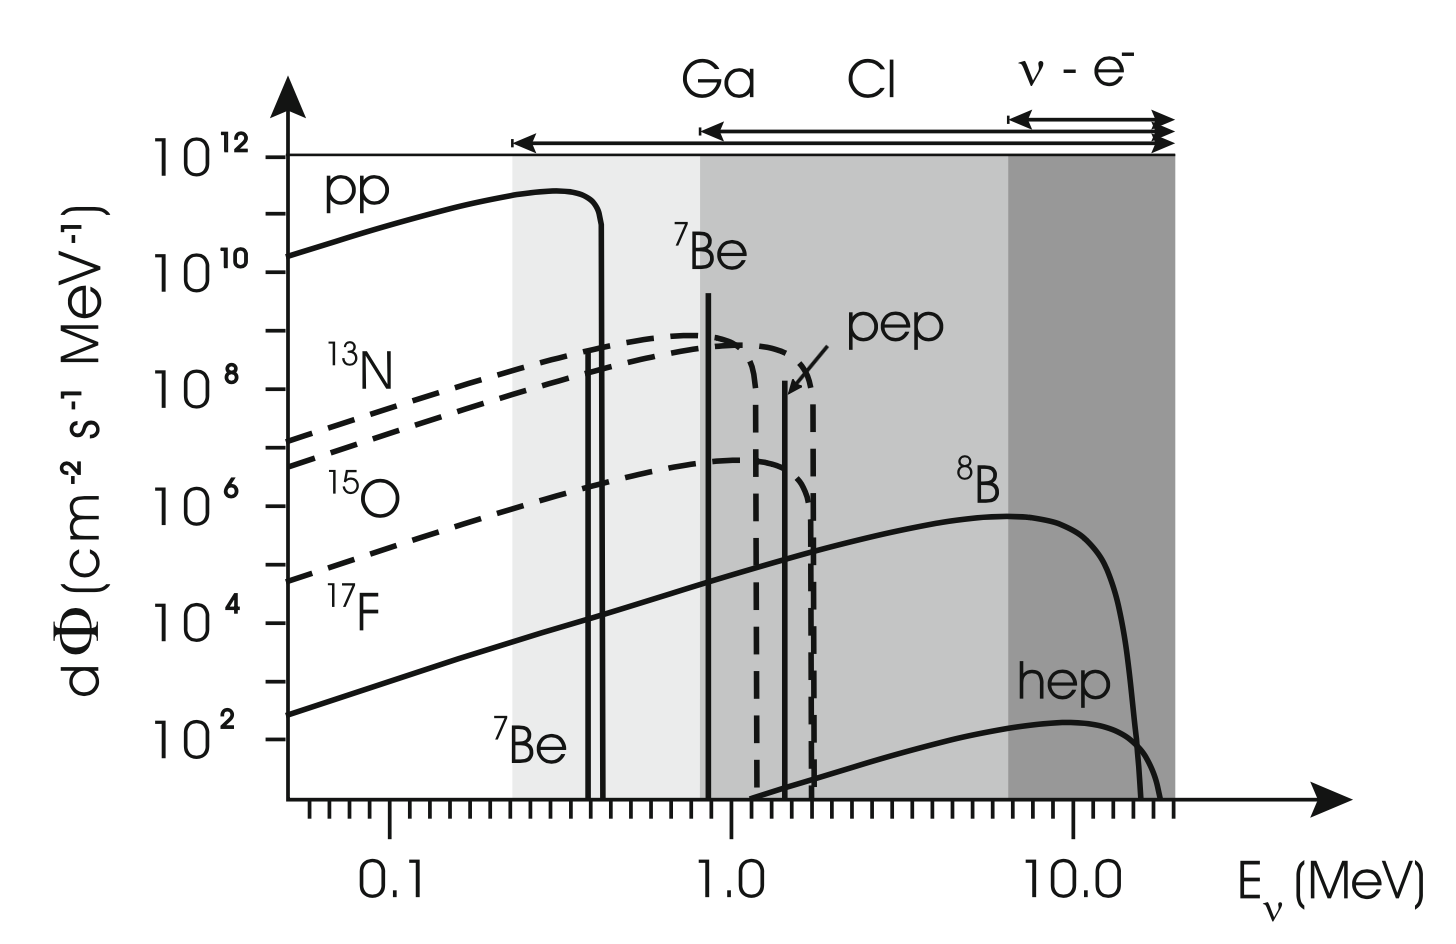
\includegraphics[width=10cm]{figures/NeutrinoSpectrum.png}}
\end{figure}

{\noindent}\textbf{The evolution of neutrino astronomy}: The following is from the brief Millennium Essay for the PASP on the evolution of neutrino astronomy from the personal perspective of John Bahcall and Raymon Davis, Jr (2000).

{\noindent}The possibility of observing solar neutrinos began to be discussed seriously following the 1958 experimental discovery by H. P. Holmgren and R. Johnston that the cross section for production of the isotope $^7$Be by the fusion reaction $^3{\rm He}+^4{\rm He}\rightarrow^7{\rm Be}+\gamma$ was more than a thousand times larger than was previously believed. This result led Willy Fowler and Al Cameron to suggest that $^8$B might be produced in the Sun in sufficient quantities by the reaction $^7{\rm Be}+p\rightarrow^8{\rm B}+\gamma$ to produce an observable flux of high energy neutrinos from $^8$B beta-decay.

{\noindent}We begin our story in 1964, when we published back-to-back papers in Physical Review Letters arguing that a 100,000 gallon detector of perchloroethylene could be built which would measure the Solar neutrino capture rate on chlorine. Our motivation was to use neutrinos to look into the interior of the Sun and thereby test directly the theory of stellar evolution and nuclear energy generation in stars. The particular development that made us realize that the experiment could be done was the theoretical discovery (by John in late 1963) that the principal neutrino absorption cross section on chlorine was 20 times larger than previously estimated due to a super-allowed nuclear transition to an excited state of argon.

{\noindent}If you have a good idea today, it likely will require many committees, many years, and many people in order to get the project from concept to observation. The situation was very different in 1964. Once the decision to go ahead was made, a very small team designed and built the experiment; the entire team consisted of Ray, Don Harmer (on leave from Georgia Tech), and John Galvin (a technician who worked part-time on the experiment). Kenneth Hoffman, a (then) young engineer, provided expert advice on technical questions. The money came out of the chemistry budget at Brookhaven National Laboratory. Neither of us remember a formal proposal ever being written to a funding agency. The total capital expenditure to excavate the cavity in the Homestake Gold Mine in South Dakota, to build the tank, and to purchase the liquid was \$0.6 million dollars (in 1965 dollars).

{\noindent}During the period 1964-1967, Fred Reines and his group worked on three Solar neutrino experiments in which recoil electrons produced by neutrino interactions would be detected by observing the associated light in an organic scintillator. Two of the experiments, which exploited the elastic scattering of neutrinos by electrons, were actually performed and led to a (higher than predicted) upper limit on the $^8$B solar neutrino flux. The third experiment, which was planned to detect neutrinos absorbed by $^7$Li, was abandoned after the initial chlorine results showed that the solar neutrino flux was low. These three experiments introduced the technology of organic scintillators into the arena of Solar neutrino research, a technique that will only finally be used in 2001 when the BOREXINO detector will begin to detect low-energy Solar neutrinos. Also during this period, John investigated the properties of neutrino electron scattering and showed that the forward peaking from $^8$B neutrinos is large, a feature that was incorporated two and half decades later in the Kamiokande (and later Super-Kamiokande) water Cerenkov detectors.

{\noindent}The first results from the chlorine experiment were published in 1968, again in a back-to-back comparison (in Physical Review Letters) between measurements and standard predictions. The initial results have been remarkably robust; the conflict between chlorine measurements and standard Solar model predictions has lasted over three decades. The main improvement has been in the slow reduction of the uncertainties in both the experiment and the theory. The efficiency of the Homestake chlorine experiment was tested by recovering carrier solutions, by producing $^{37}$Ar in the tank with neutron sources, and by recovering $^{36}$Cl inserted in a tank of perchloroethylene. The Solar model was verified by comparison with precise helioseismological measurements.

{\noindent}For much more than two decades, the best estimates for the observational and for the theoretical prediction have remained essentially constant. The discrepancy between the standard Solar model predictions and the chlorine observations became widely known as the \textbf{Solar neutrino problem}. 

{\noindent}Very few people worked on Solar neutrinos during the period 1968-1988. The chlorine experiment was the only solar neutrino experiment to provide data in these two decades. It is not easy for us to explain why this was the cas;; we certainly tried hard to interest others in doing different experiments, and we gave many joint presentations about what came to be known as the solar neutrino problem. Each of us had one principal collaborator during this long period, Bruce Cleveland (experimental) and Roger Ulrich (Solar models). A large effort to develop a chlorine experiment in the Soviet Union was led by George Zatsepin, but it was delayed by the practical difficulties of creating a suitable underground site for the detector. Eventually, the effort was converted into a successful gallium detector, SAGE, led by Vladimir Gavrin and Tom Bowles, that gave its first results in 1990.

{\noindent}Only 1 year after the first (1968) chlorine results were published, Vladimir Gribov and Bruno Pontecorvo proposed that the explanation of the Solar neutrino problem was that neutrinos oscillated between the state in which they were created and a more difficult to detect state. This explanation, which is the consensus view today, was widely disbelieved by nearly all the particle physicists we talked to in those days. In the form in which Solar neutrino oscillations were originally proposed by Gribov and Pontecorvo, the process required that the mixing angles between neutrino states be much larger than the quark mixing angles, something which most theoretical physicists believed, at that time, was unlikely. Ironically, a flood of particle theory papers explained, more or less ``naturally,'' the large neutrino mixing angle that was decisively demonstrated 30 years later in the Super-Kamiokande atmospheric neutrino experiment.

{\noindent}One of the most crucial events for early Solar neutrino research occurred in 1968 while we were relaxing in the Sun after a swim at the Caltech pool. Gordon Garmire (now a PI for the Chandra X-ray Observatory) came up to Ray, introduced himself, and said he had heard about the chlorine experiment. He suggested to Ray that it might be possible to reduce significantly the background by using pulse rise-time discrimination, a technique used for proportional counters in space experiments. The desired fast-rising pulses from $^{37}$Ar Auger electrons are different from the slower rising pulses from a background gamma or cosmic ray. Ray went back to Brookhaven and asked the local electronic experts if it would be possible to implement this technique for the very small counters he used. The initial answer was that the available amplifiers were not fast enough to be used for this purpose with the small Solar neutrino counters. But, in about a year three first-class electronic engineers at Brookhaven, Veljko Radeca, Bob Chase, and Lee Rogers, were able to build electronics fast enough to be used to measure the rise time in Ray's counters.

{\noindent}This ``swimming pool'' improvement was crucial for the success of the chlorine experiment and the subsequent radio-chemical gallium solar neutrino experiments, SAGE, GALLEX, and GNO. Measurements of the rise time as well as the pulse energy greatly reduce the background for radio-chemical experiments. The backgrounds can be as low as one event in 3 months. 

{\noindent}In 1978, after a decade of disagreement between the Homestake neutrino experiment and standard Solar model predictions, it was clear to everyone that the subject had reached an impasse and a new experiment was required. The chlorine experiment is, according to standard Solar model predictions, sensitive primarily to neutrinos from a rare fusion reaction that involves $^8$B neutrinos. These neutrinos are produced in only $2$ of every $10^4$ terminations of the basic p-p fusion chain. In the early part of 1978, there was a conference of interested scientists who got together at Brookhaven to discuss what to do next. The consensus decision was that we needed an experiment that was sensitive to the low-energy neutrinos from the fundamental p-p reaction.

{\noindent}The only remotely practical possibility appeared to be another radio-chemical experiment, this time with $^{71}$Ga (instead of $^{37}$Cl) as the target. But, a gallium experiment (originally proposed by the Russian theorist V. A. Kuzmin in 1965) was expensive; we needed about 3 times the world's annual production of gallium to do a useful experiment. In an effort to generate enthusiasm for a gallium experiment, we wrote another Physical Review Letters paper, this time with a number of interested experimental colleagues. We argued that a gallium detector was feasible and that a gallium measurement, which would be sensitive to the fundamental p-p neutrinos, would distinguish between broad classes of explanations for the discrepancy between prediction and observation in the $^{37}$Cl experiment. Over the next $5$ or $6$ years, the idea was reviewed a number of times in the United States, always very favorably. The Department of Energy (DOE) appointed a blue ribbon panel headed by Glen Seaborg that endorsed enthusiastically both the experimental proposal and the theoretical justification.

{\noindent}To our great frustration and disappointment, the gallium experiment was never funded in the United States, although the experimental ideas that gave rise to the Russian experiment (SAGE) and the German-French-Italian-Israeli-US experiment (GALLEX) originated largely at Brookhaven. Physicists strongly supported the experiment and said the money should come out of the astronomy budget; astronomers said it was great physics and should be supported by the physicists. DOE could not get the nuclear physics and the particle physics sections to agree on who had the financial responsibility for the experiment. In a desperate effort to break the deadlock, John was even the PI of a largely Brookhaven proposal to the National Science Foundation (which did not support proposals from DOE laboratories). A pilot experiment was performed with $1.3$ tons of gallium by an international collaboration (Brookhaven, University of Pennsylvania; Max Planck Institute, Heidelberg; Institute for Advanced Study, Princeton; and the Weizmann Institute) which developed the extraction scheme and the counters eventually used in the GALLEX full-scale experiment.

{\noindent}In strong contrast to what happened in the United States, Moissey Markov, the head of the Nuclear Physics Division of the Russian Academy of Sciences, helped establish a neutrino laboratory within the Institute for Nuclear Research, participated in the founding of the Baksan neutrino observatory, and was instrumental in securing $60$ tons of gallium free to Russian scientists for the duration of a Solar neutrino experiment. The Russian-American gallium experiment (SAGE) went ahead under the leadership of Vladimir Gavrin, George Zatsepin (Institute for Nuclear Research, Russia), and Tom Bowles (Los Alamos), and the mostly European experiment (GALLEX) was led by Till Kirsten (Max Planck Institute, Germany). Both experiments had a strong but not primary US participation.

{\noindent}The two gallium experiments were performed in the decade of the 1990s and gave very similar results, providing the first experimental indication of the presence of p-p neutrinos. Both experiments were tested by measuring the neutrino rate from an intense laboratory radioactive source.

{\noindent}There were two dramatic developments in the Solar neutrino saga, one theoretical and one experimental, before the gallium experiments produced observational results. In 1985, two Russian physicists proposed an imaginative solution of the Solar neutrino problem that built upon the earlier work of Gribov and Pontecorvo and, more directly, the insightful investigation by Lincoln Wolfenstein (of Carnegie Mellon University). Stanislav Mikheyev and Alexei Smirnov showed that if neutrinos have masses in a relatively wide range, then a resonance phenomenon in matter (now universally known as the \textbf{MSW effect}) could convert efficiently many of the electron-type neutrinos created in the interior of the Sun to more difficult to detect muon and tau neutrinos. The MSW effect can work for small or large neutrino mixing angles. Because of the elegance of the theory and the possibility of explaining the experimental results with small mixing angles (analogous to what happens in the quark sector), physicists immediately began to be more sympathetic to particle physics solutions to the Solar neutrino problem. More importantly, they became enthusiasts for new Solar neutrino experiments.

{\noindent}The next big breakthrough also came from an unanticipated direction. The Kamiokande water Cerenkov detector was developed to study proton decay in a mine in the Japanese Alps; it set an important lower limit on the proton lifetime. In the late 1980s, the detector was converted by its Japanese founders, Masatoshi Koshiba and Yoji Totsuka, together with some American colleagues (Gene Beier and Al Mann of the University of Pennsylvania), to be sensitive to the lower energy events expected from Solar neutrinos. With incredible foresight, these experimentalists completed in late 1986 their revisions to make the detector sensitive to Solar neutrinos, just in time to observe the neutrinos from SN 1987a emitted in the LMC 170,000 years earlier. (Supernova and Solar neutrinos have similar energies, $\sim10\,{\rm MeV}$, much less than the energies that are relevant for proton decay.) In 1996, a much larger water Cerenkov detector (with 50,000 tons of pure water) began operating in Japan under the leadership of Yoji Totsuka, Kenzo Nakamura, Yoichiro Suzuki (from Japan), and Jim Stone and Hank Sobel (from the United States).

{\noindent}So far, five experiments have detected solar neutrinos in approximately the numbers (within a factor of $2$ or $3$) and in the energy range ($<15\,{\rm MeV}$) predicted by the standard Solar model. This is a remarkable achievement for Solar theory since the $^8$B neutrinos that are observed primarily in three of these experiments (chlorine, Kamiokande, and its successor Super-Kamiokande) depend upon approximately the $25^{\rm th}$ power of the central temperature. The same set of nuclear fusion reactions that are hypothesized to produce the Solar luminosity also give rise to Solar neutrinos. Therefore, these experiments establish empirically that the Sun shines by nuclear fusion reactions among light elements in essentially the way described by Solar models.

{\noindent}Nevertheless, all of the experiments disagree quantitatively with the combined predictions of the standard Solar model and the standard theory of electroweak interactions (which implies that nothing much happens to the neutrinos after they are created). The disagreements are such that they appear to require some new physics that changes the energy spectrum of the neutrinos from different fusion sources.

{\noindent}Solar neutrino research today is very different from what it was three decades ago. The primary goal now is to understand the neutrino physics, which is a prerequisite for making more accurate tests of the neutrino predictions of Solar models. Solar neutrino experiments today are all large international collaborations, each typically involving of order $10^2$ physicists. Nearly all of the new experiments are electronic, not radio-chemical, and the latest generation of experiments measure typically several thousand events per year (with reasonable energy resolution), compared to rates that were typically $25-50$ per year for the radio-chemical experiments (which have no energy resolution, only an energy threshold). Solar neutrino experiments are currently being carried out in Japan (Super-Kamiokande, in the Japanese Alps), in Canada (SNO, which uses a kiloton of heavy water in Sudbury, Ontario), in Italy (BOREXINO, ICARUS, and GNO, each sensitive to a different energy range and all operating in the Gran Sasso Underground Laboratory), in Russia (SAGE, in the Caucasus region), and in the United States (Homestake chlorine experiment). The SAGE, chlorine, and GNO experiments are radio-chemical; all the others are electronic.

{\noindent}Since 1985, the chlorine experiment has been operated by the University of Pennsylvania under the joint leadership of Ken Lande and Ray Davis. Lande and Paul Wildenhain have introduced major improvements in the extraction and measurement systems, making the chlorine experiment a valuable source of new precision data. 

{\noindent}The most challenging and important frontier for Solar neutrino research is to develop experiments that can measure the energies of individual low-energy neutrinos from the basic p-p reaction, which constitutes (we believe) more than $90\%$ of the Solar neutrino flux. 

{\noindent}Solar neutrino research is a community activity. Hundreds of experimentalists have collaborated to carry out difficult, beautiful measurements of the elusive neutrinos. Hundreds of other researchers helped redefine the Solar model predictions, measuring accurate nuclear and Solar parameters and calculating input data such as opacities and equation of state.

{\noindent}Three people played special roles. Hans Bethe was the architect of the theory of nuclear fusion reactions in stars, as well as our mentor and hero. Willy Fowler was a powerful and enthusiastic supporter of each new step, and his keen physical insight motivated much of what was done in Solar neutrino research. Bruno Pontecorvo opened everyone's eyes with his original insights, including his early discussion of the advantages of using chlorine as a neutrino detector and his suggestion that neutrino oscillations might be important.

{\noindent}In the next decade, neutrino astronomy will move beyond our cosmic neighborhood and, we hope, will detect distant sources. The most likely candidates now appear to be gamma-ray bursts. If the standard fireball picture is correct and if gamma-ray bursts produce the observed highest energy cosmic rays, then very high energy ($10^{15}\,{\rm eV}$) neutrinos should be observable with a ${\rm km}^2$ detector. Experiments with the capability to detect neutrinos from gamma-ray bursts are being developed at the South Pole (AMANDA and ICECUBE), in the Mediterranean Sea (ANTARES, NESTOR), and even in space.

{\noindent}Looking back on the beginnings of solar neutrino astronomy, one lesson appears clear to us: if you can measure something new with reasonable accuracy, then you have a chance to discover something important. The history of astronomy shows that very likely what you will discover is not what you were looking for. It helps to be lucky. 

\subsubsection{Follow-up Questions}

\begin{itemize}
    \item Can neutrinos account for all of the dark matter in the Universe?
    \item If there was a fourth neutrino flavour, how would we detect it?
    \item Why is the first step of the p-p chain not where we looked for neutrino signatures? (i.e., not energetic enough)
\end{itemize}

% --------------------------------------------------------------
%               8. 
% --------------------------------------------------------------

\newpage
\subsection{Question 8}

Why is nuclear fusion stable inside a main-sequence star? Under what conditions is nuclear fusion unstable? Give examples of actual objects.

\subsubsection{Short answer}

Answer.

\subsubsection{Additional context}

Additional context.

\subsubsection{Follow-up Questions}

\begin{itemize}
    \item Can main sequence stars have unstable nuclear fusion?
    \item If I suddenly increase the core temperature of a star by 20\%, how quickly does the star respond?
    \item What happens when you ignite fusion in a white dwarf? Explain using explicit thermodynamics what happens when you turn up the temperature or reaction rate in the core of the star (i.e. explain adiabatic expansion and contraction).
\end{itemize}

% --------------------------------------------------------------
%               9. 
% --------------------------------------------------------------

\newpage
\subsection{Question 9}

Why do neutrons inside a neutron star not decay into protons and electrons?

\subsubsection{Short answer}

Answer.

\subsubsection{Additional context}

Additional context.

\subsubsection{Follow-up Questions}

\begin{itemize}
    \item What sort of products come from NS-NS mergers?
    \item What are typical photon energies emitted from each of these scenarios?
\end{itemize}

% --------------------------------------------------------------
%               10. 
% --------------------------------------------------------------

\newpage
\subsection{Question 10}

What is the typical temperature of matter accreting on a star, a white dwarf, a neutron star, a stellar mass black hole, and a supermassive black hole? In what wavelength range would one best find examples of such sources?

\subsubsection{Short answer}

Answer.

\subsubsection{Additional context}

Additional context.

\subsubsection{Follow-up Questions}

\begin{itemize}
    \item How does the accretion process work?
    \item If you don't assume a blackbody, and just dump a bunch of material onto a star and it can't radiate away, what is the maximum temperature it can reach?
\end{itemize}

% --------------------------------------------------------------
%               11. 
% --------------------------------------------------------------

\newpage
\subsection{Question 11}

You don't usually need to cool down the detectors for short wavelength (e.g., X-ray) observations, but it's critical to cool down the detectors in long wavelength (e.g., far-IR) observations. Why is this, and why is it not necessary for radio observations?

\subsubsection{Short answer}

Answer.

\subsubsection{Additional context}

Additional context.
% --------------------------------------------------------------
%               12. 
% --------------------------------------------------------------

\newpage
\subsection{Question 12}

Compare the S/N ratios between the following two cases where photon noise is dominant (assume an unresolved point source): [A] 1-minute exposure with a 10-m telescope; [B] 10-minute exposure with a 1-m telescope.

\subsubsection{Short answer}

Answer.

\subsubsection{Additional context}

Additional context.

% --------------------------------------------------------------
%               13. 
% --------------------------------------------------------------

\newpage
\subsection{Question 13}

Describe linear and circular polarizations of electromagnetic waves and give examples of their relevance to astronomical observations.

\subsubsection{Short answer}

Answer.

\subsubsection{Additional context}

{\noindent}Electromagnetic waves can be characterized by four properties: intensity, frequency, direction of propagation, and polarization state. Figure \ref{fig:empol} shows why polarization is considered an important characteristic of an EM wave. The oscillating electric and magnetic field vectors will have a particular orientation at a given instant in time (Figure \ref{fig:empol}a). Figure \ref{fig:empol}b shows how the polarization state of a wave changes its orientation over time. If the wave oscillates in a single plane, the wave is said to be \textbf{linearly polarized} (see Figure \ref{fig:polarizationtypes}b), while a wave composed of two plane waves of equal amplitude but differing in phase by $90^\circ$ is \textbf{circularly polarized} (Figure \ref{fig:polarizationtypes}a). If two plane waves have differing amplitudes or a phase difference that is not $90^\circ$, then the resultant wave is \textbf{elliptically polarized} (Figure \ref{fig:polarizationtypes}c).

\begin{figure}[h]
    \floatbox[{\capbeside\thisfloatsetup{capbesideposition={right,top},capbesidewidth=4cm}}]{figure}[\FBwidth]
    {\caption{\footnotesize{\\This figure shows (a) an EM wave and (b) how its polarization changes as it propagates along the $z$-axis. At position $1$, the electric vector is pointing in the $x$-direction, but at point $2$, some time in the future, the electric vector is pointing in the $y$-direction. One complete revolution has been completed by point $4$, and points $5-8$ repeat the cycle. The wave is circularly polarized as there are equal amplitude components in both the $x$ and $y$ planes. This figure is reproduced from \href{http://astronomyonline.org}{http://astronomyonline.org}. Figure taken from Newton-McGee (2009).}}
    \label{fig:empol}}
    {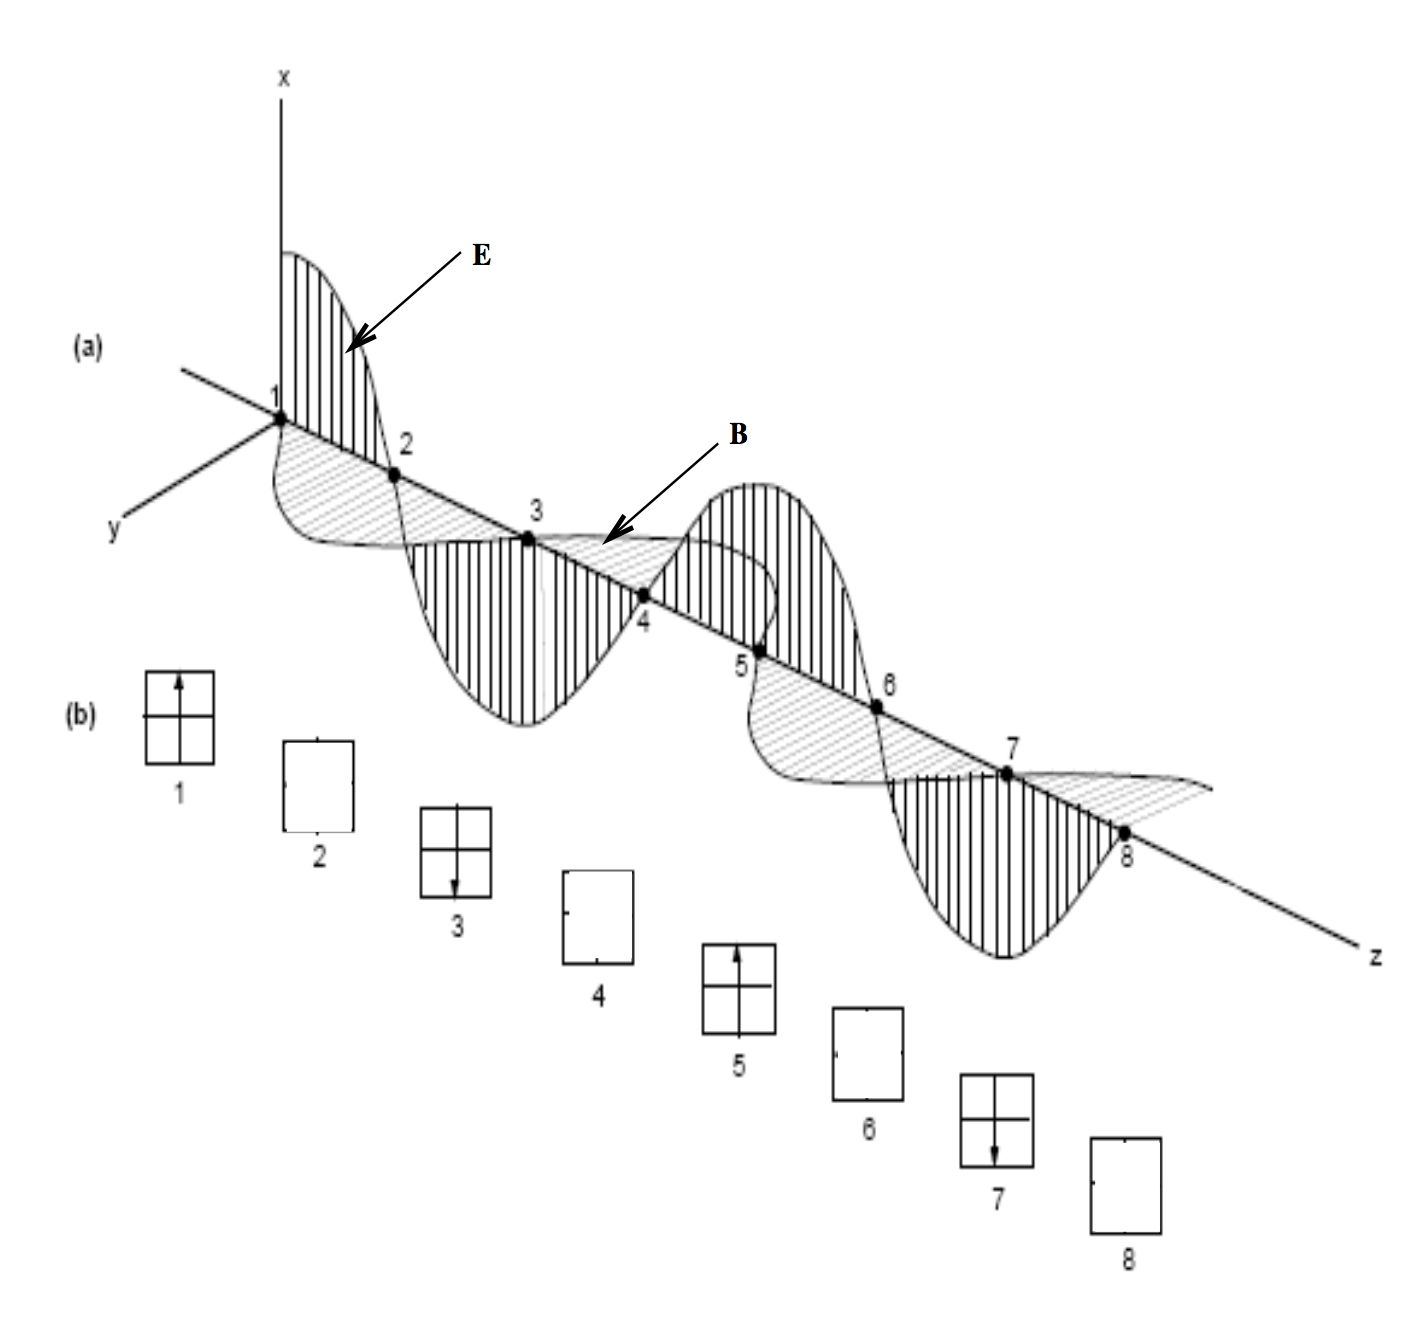
\includegraphics[width=10cm]{figures/EMpol.png}}
\end{figure}

{\noindent}There are many ways of describing the polarization state of an EM wave. If we begin with a quasi-monochromatic wave propagating in the $z$-direction, it can be resolved into three Cartesian components ($x,y,z$):

\begin{align*}
    E_x &= a_1(t)\exp[i(\phi_1(t)-2\pi\nu t)] ~ [{\rm N\,C^{-1}}], \\
    E_y &= a_2(t)\exp[i(\phi_2(t)-2\pi\nu t)] ~ [{\rm N\,C^{-1}}], \\
    E_z &= 0 ~ [{\rm N\,C^{-1}}],
\end{align*}

{\noindent}where $E$ is the magnitude of the electric field vector, $a_1$ and $a_2$ are the amplitudes, and $\phi_1$ and $\phi_2$ are the phases of the component waves.

\begin{figure}[t]
    \centering
    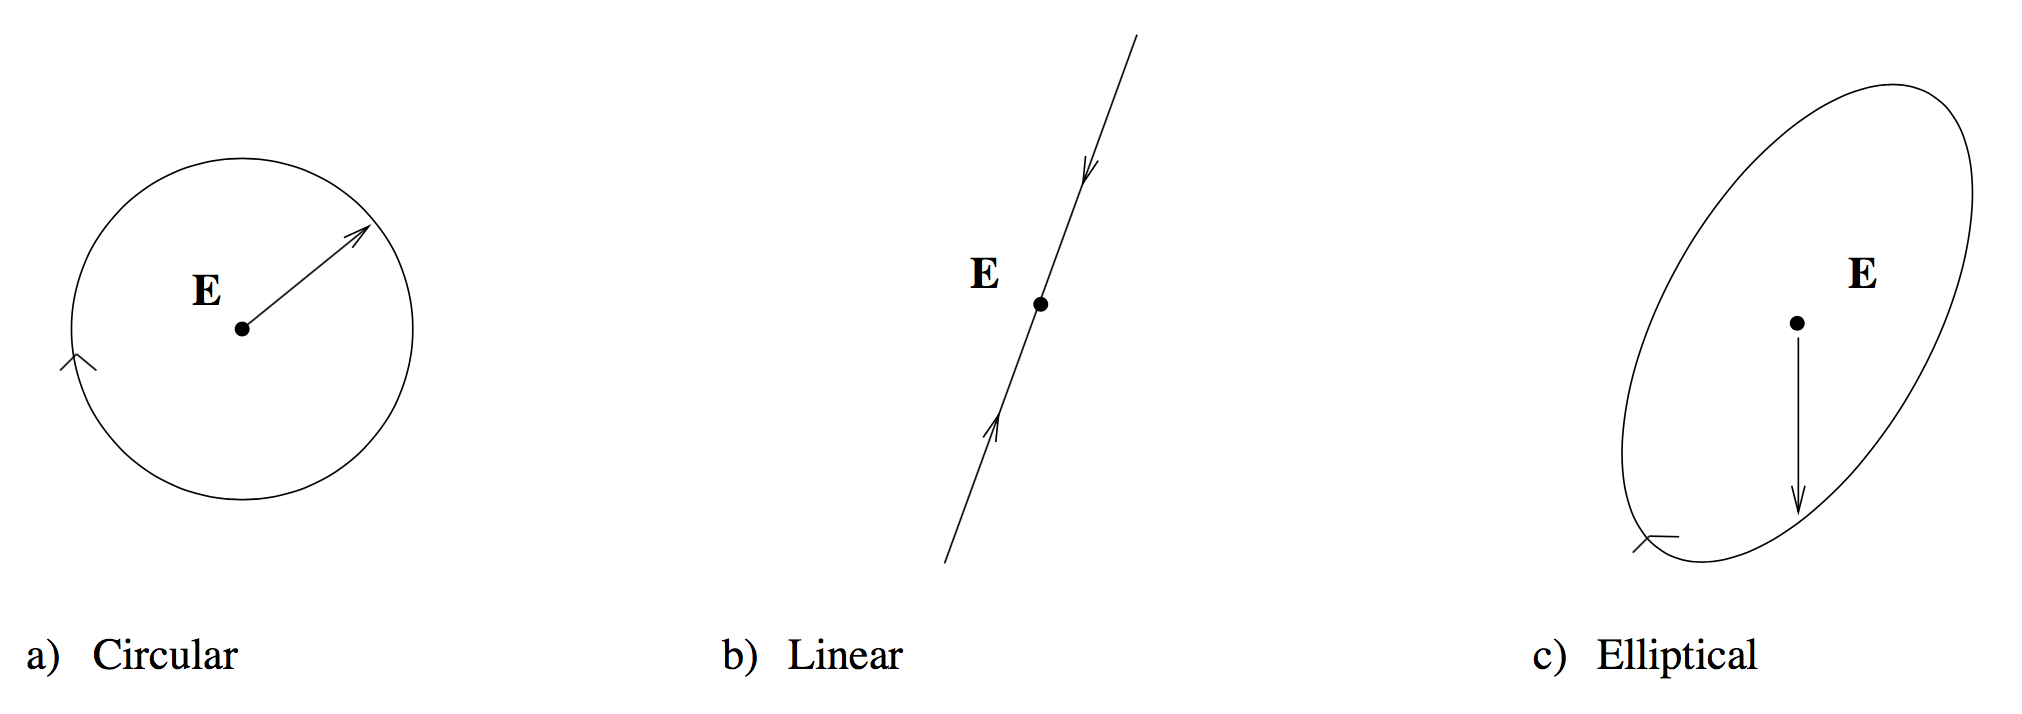
\includegraphics[width=12cm]{figures/PolarizationTypes.png}
    \caption{\footnotesize{End on view of the trace of the tip of the electric vector for: (a) circularly polarized radiation, (b) linearly polarized radiation, and (c) elliptically polarized radiation. This figure is adapted from Cotton (1999). Figure taken from Newton-McGee (2009).}}
    \label{fig:polarizationtypes}
\end{figure}

{\noindent}The polarization states of the wave are described by the \textbf{Stokes parameters} are:

\begin{align*}
    I &= \langle{a_1^2}\rangle + \langle{a_2^2}\rangle ~ [{\rm N\,C^{-1}}] \\
    Q &= \langle{a_1^2}\rangle - \langle{a_2^2}\rangle ~ [{\rm N\,C^{-1}}] \\
    U &= 2\langle{a_1a_2\cos\phi}\rangle ~ [{\rm N\,C^{-1}}] \\
    V &= 2\langle{a_1a_2\sin\phi}\rangle ~ [{\rm N\,C^{-1}}].
\end{align*}

{\noindent}where $\langle\rangle$ represents the time averaged quantity. \textbf{Stokes} $\mathbf{I}$ is a measurement of the total intensity of the wave, \textbf{Stokes} $\mathbf{Q}$ and $\mathbf{U}$ together describe the linearly polarized components while \textbf{Stokes} $\mathbf{V}$ represents the circularly polarized component of the wave. If $V>0$ then the wave is right-handed circularly polarized (RCP), while if $V<0$ then the polarization is left-handed circularly polarized (LCP). 

{\noindent}From correctly calibrated Stokes images, useful polarization images can be produced. Customarily, three linear polarization parameters are constructed: the \textbf{polarized intensity} ($P$) image, the \textbf{polarization angle} ($\chi$) image, and the \textbf{polarization fraction} ($p$) image. These are formed from the Stokes $Q$ and $U$ images in the following manner:

\begin{align*}
    P &= \sqrt{Q^2+U^2} ~ [{\rm Jy}] \\
    \chi &= \frac{1}{2} \arctan \left(\frac{U}{Q}\right) ~ [{\rm rad}] \\
    p &= \frac{\sqrt{Q^2+U^2}}{I} ~ [{\rm dimensionless}].
\end{align*}

The polarization of electromagnetic radiation is fundamental to many physical processes including: how bees view the world, why rainbows exist, and many astrophysical phenomena including:

\begin{itemize}
    \item synchrotron radiation (linear polarization);
    \item CMB polarization (linear and circular polarization);
    \item dust polarization (linear polarization);
    \item starlight polarization (linear polarization);
    \item astrophysical magnetic fields (linear polarization);
    \item Faraday rotation (linear polarization).
\end{itemize}


% --------------------------------------------------------------
%               14. 
% --------------------------------------------------------------

\newpage
\subsection{Question 14}

What's the field of view of a $2{\rm K}\,\times\,2{\rm K}$ CCD camera on a $5\,{\rm m}$ telescope with $f/16$ focal ratio? The pixel size of the CCD is $20\,\mu$m. Now, let’s bring this to a $10\,{\rm m}$ telescope with the same focal ratio. Explain how the field of view changes on the $10\,{\rm m}$ telescope (compared to that of the $5\,{\rm m}$ telescope) based on the Etendue conservation rule.

\subsubsection{Short answer}

Answer.

\subsubsection{Additional context}

Additional context.

\subsubsection{Follow-up Questions}

\begin{itemize}
    \item If you wanted a smaller FOV with the same size telescope, what would you change?
\end{itemize}

% --------------------------------------------------------------
%               15. 
% --------------------------------------------------------------

\newpage
\subsection{Question 15}

Sketch and give the equations for each of the following distributions: 1. Gaussian (Normal distribution); 2. Poisson distribution; 3. Log-normal distribution. Give two examples from astrophysics where each of these distributions apply.

\subsubsection{Short answer}

Answer.

\subsubsection{Additional context}

\textbf{Accuracy versus precision}: It is important to distinguish between the terms \textit{accuracy} and \textit{precision}. The \textbf{accuracy} of an experiment is a measure of how close the result of the experiment is to the true value; the \textbf{precision} is a measure of how well the result has been determined, without reference to its agreement with the true value. The precision is also a measure of the \textbf{reproducibility} of the result in a given experiment. The distinction between \textit{accuracy} and \textit{precision} is illustrated by the two sets of measurements in Figure \ref{fig:precisionaccuracy} where the straight line on each graph shows the expected relation between the dependent variable $y$ and the independent variable $x$. In both graphs, the scatted of the data points is a reflection of uncertainties in the measurements, consistent with the error bars on the points. The data in Figure \ref{fig:precisionaccuracy}a have been measured to a high degree of \textit{precision} as illustrated by the small error bars, and are in excellent agreement with the expected variation of $y$ with $x$, but are clearly \textit{inaccurate}, deviating from the line by a constant offset. On the other hand, the data points in Figure \ref{fig:precisionaccuracy}b are rather \textit{imprecise} as illustrated by the large error bars, but are scattered around the predicted distribution.

\begin{figure}[h]
    \floatbox[{\capbeside\thisfloatsetup{capbesideposition={right,top},capbesidewidth=4cm}}]{figure}[\FBwidth]
    {\caption{\footnotesize{\\Illustration of the difference between precision and accuracy. \textbf{(a)} Precise but inaccurate data. \textbf{(b)} Accurate but imprecise data. True values are represented by the straight lines. Figure taken from Bevington \& Robinson (2003).}}
    \label{fig:precisionaccuracy}}
    {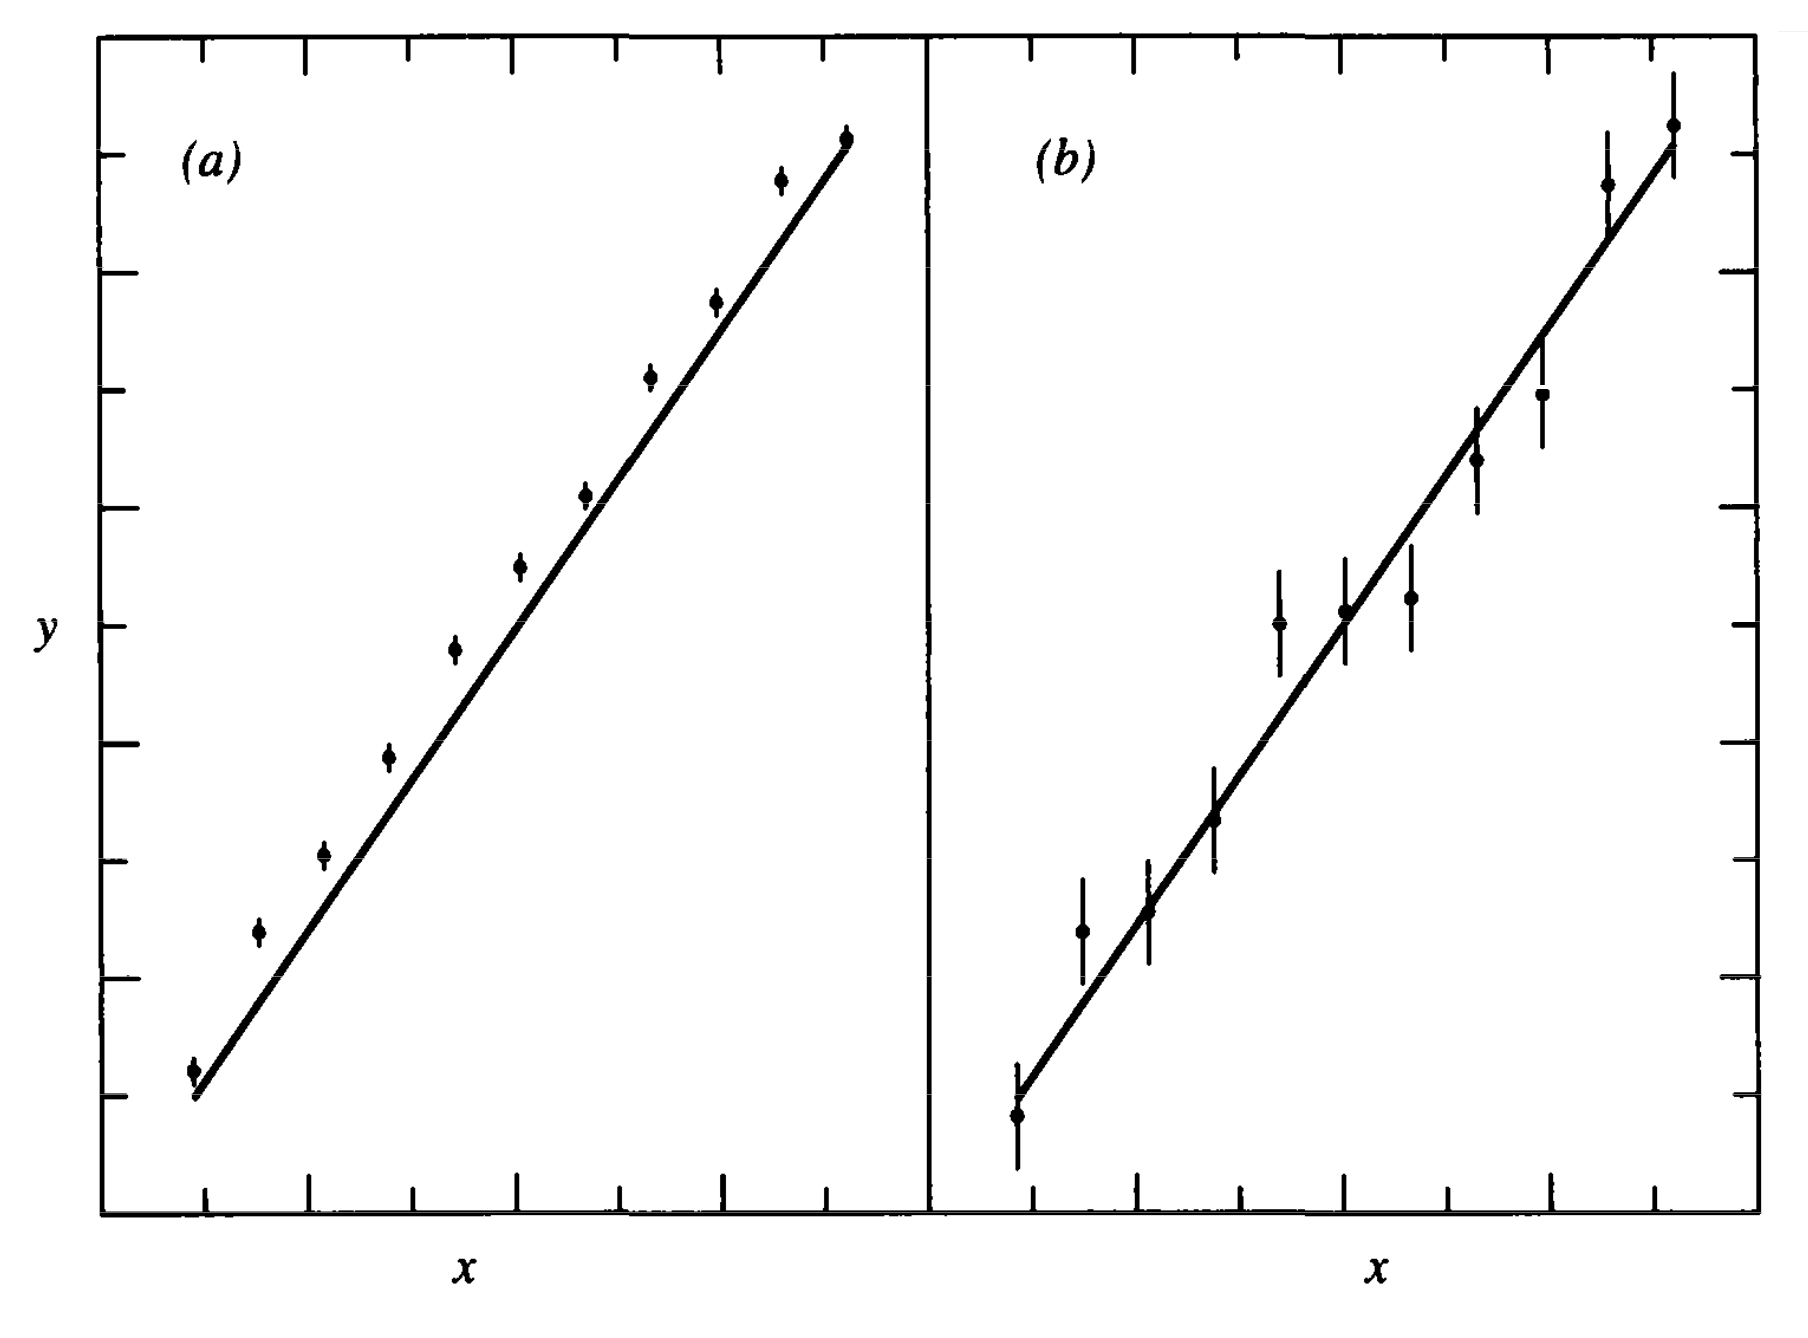
\includegraphics[width=12cm]{figures/PrecisionAccuracy.png}}
\end{figure}

{\noindent}It is obvious that we must consider the accuracy and precision simultaneously for any experiment. It would be a waste of time and energy to determine a result with high precision if we knew that the result would be highly inaccurate. Conversely, a result cannot be considered to be extremely accurate if the precision is low. In general, when we know the \textbf{uncertainty} or \textbf{error} of an experimental result, we are referring to the precision with which that result has been determined. \textbf{Absolute precision} indicates the magnitude of the uncertainty in the result in the same units as the result; \textbf{relative precision} indicates the uncertainty in terms of a fraction of the value of the result.

{\noindent}\textbf{Systematic errors}: The accuracy of an experiment, as we have defined it, is generally dependent on how well we can control or compensate for \textbf{systematic errors}, or errors that will make our result different from the ``true'' value with reproducible discrepancies. Errors of this type are not easy to detect and not easily studied by statistical analysis. They may result from faulty calibration of equipment or bias on the part of the observer. They must be estimated from an analysis of the experimental conditions and techniques. A major part of the planning of an experiment should be devoted to understanding and reproducing sources of systematic errors.

{\noindent}\textbf{Random errors}: The precision of an experiment depends upon how well we can overcome \textbf{random errors}, or fluctuations in observations that yield different results each time the experiment is repeated, and thus requires repeated experimentation to yield precise results. A given accuracy implies an equivalent precision and, therefore, also depends to some extent on random errors. 

{\noindent}The problem or reducing random errors is essentially one of improving the experimental method and refining the techniques, as well as simply repeating experiment. If the random errors result from instrumental uncertainties, they may be reduced by using more reliable and more precise measuring techniques. If the random errors result from statistical fluctuations in a limited number of measurements, they may be reduced by making more measurements. There are, however, practical limits to these improvements. 

{\noindent}\textbf{Mean, median, and mode}: The \textbf{mean} $\bar{x}$ of an experimental distribution is given as the sum of $N$ determinations of $x_i$ od the quantity $x$ divided by the number of determinations

\begin{align*}
    \bar{x} \equiv \frac{1}{N} \sum x_i ~ [{\rm function}],
\end{align*}

{\noindent}and the \textbf{mean of the parent population} $\mu$ is defined as the limit

\begin{align*}
    \mu \equiv \lim_{N\rightarrow\infty}\left( \frac{1}{N} \sum x_i \right) ~ [{\rm function}].
\end{align*}

{\noindent}The mean is therefore equivalent to the \textbf{centroid} or \textbf{average} value of the quantity $x$.

{\noindent}\textbf{Deviations}: The deviation $d_i$ of any measurement $x_i$ from the mean $\mu$ of the parent population is defined as the difference between $x_i$ and $\mu$:

\begin{align*}
    d_i \equiv x_i - \mu ~ [{\rm function}].
\end{align*}

{\noindent}For computational purposes, deviations are generally defined with respect to the mean, rather than the median or most probable value. If $\mu$ is the true value of the quantity, $d_i$ is also the true error in $x_i$.

{\noindent}The average of the deviations $d_i$ must vanish by virtue of the definition of the mean:

\begin{align*}
    \lim_{N\rightarrow\infty} \bar{d_i} = \lim_{N\rightarrow\infty} \left[ \frac{1}{N} \sum(x_i-\mu) \right] = \lim_{N\rightarrow\infty}\left(\frac{1}{N}\sum x_i\right) - \mu = 0 ~ [{\rm function}].
\end{align*}

{\noindent}The \textbf{average deviation} $\alpha$, therefore, is defined as the absolute values of the deviations:

\begin{align*}
    \alpha \equiv \lim_{N\rightarrow\infty}\left[ \frac{1}{N} \sum \left\lvert x_i-\mu\right\rvert \right] ~ [{\rm function}].
\end{align*}

{\noindent}The average deviation is a measure of the \textbf{dispersion}of the expected observations about the mean. The presence of the absolute value signs makes its use inconvenient for statistical analysis.

{\noindent}A parameter that is easier to use analytically and that can be justified fairly well on theoretical grounds to be a more appropriate measure of the dispersion of the observations is the \textbf{standard deviation} $\sigma$. The \textbf{variance} $\sigma^2$ is defined as the limit of the average of the squares of the deviations from the mean $\mu$:

\begin{align*}
    \sigma^2 \equiv \lim{N\rightarrow\infty} \left[\frac{1}{N}\sum(x_i-\mu)^2\right] = \lim_{N\rightarrow\infty} \left(\frac{1}{N}\sum x_i^2\right)-\mu^2 ~ [{\rm function}]
\end{align*}

{\noindent}and the standard deviation $\sigma$ is the square root if the variance. Note that the second form of the variance shown above is often described as the ``average of the squares minus the square of the average''. The standard deviation of the \textbf{root mean square} of the deviation, and is associated with the \textbf{second moment} of the date about the mean. The corresponding expression for the variance $s^2$ of the sample population is given by

\begin{align*}
    s^2 \equiv \frac{1}{N} \sum (x_i-\bar{x})^2 ~ [{\rm function}]
\end{align*}

{\noindent}where the factor of $N-1$, rather than $N$, is required in the denominator to account for the fact that the parameter $\bar{x}$ has been determined from the data and not independently. We note that the symbol $\sigma$ (instead of $s$) is often used to represent the best estimate of the standard deviation of the parent distribution determined from a sample distribution.

{\noindent}\textbf{Significance}: The mean $\mu$ and the standard deviation $\sigma$, as well as the median, the most probable value, and the average deviation, are all parameters that characterize the information we are seeking when we perform an experiment. Often we wish to describe our distribution in terms of just the mean and standard deviation. Th mean may not be exactly equal to the datum in question if the parent distribution is not symmetrical about the mean, but it should have the same characteristics. If a more detailed description is desired, it may be useful to compute \textbf{higher moments about the mean}.

{\noindent}In general, the best we can say about the mean is that it is one of the parameters that specifies the probability distribution: it has the same units as the ``true'' value and, in accordance with convention, we shall consider it to be the best estimate of the ``true'' value under the prevailing experimental conditions.

{\noindent}The variance $s^2$ and the standard deviation $s$ characterize the uncertainties associated with our experimental attempts to determine the ``true'' values. For a given number of observations, the uncertainty in determining the mean of the parent distribution is proportional to the standard deviation of that distribution. The standard deviation $s$ is, therefore, an appropriate measure of the uncertainty due to fluctuations in the observations in our attempt to determine the ``true'' value.

{\noindent}Although, in general, the distribution resulting from purely statistical errors can be described well by the two parameters, the mean and the standard deviation, we should be aware that, at distances of a few standard deviations from the mean of an experimental distribution, non-statistical errors may dominate. In especially severe cases, it may be preferable to describe the spread of the distribution in terms of the average deviation, rather than the standard deviation, because the latter tends to de-emphasize measurements that are far from the mean. There are also distributions for which the variance does not exist. The average deviation or some other quantity must be used as a parameter to indicate the spread of the distribution in such cases. 

{\noindent}\textbf{Probability distributions}: Of the many probability distributions that are involved in the analysis of experimental data, three play a fundamental role: the binomial distribution, the Poisson distribution, and the Gaussian distribution. Of these, the \textbf{Gaussian, or normal error, distribution}, is undoubtedly the most important in statistical analysis of data. Practically, it is useful because it seems to describe the distribution of random observations for many experiments, as well as describing the distributions obtained when we try to estimate the parameters of most other probability distributions. 

{\noindent}The \textbf{Poisson distribution} is generally appropriate for counting experiments where the data represents the number of items or events observed per unit time interval. It is important in the study of random processes such as those associated with the radioactive decay of elementary particles or nuclear states, and is also applied to data that have been sorted into ranges to form a frequency table or a histogram. 

{\noindent}The \textbf{binomial distribution} is generally applied to experiments in which the result is one of a small number of possible final states, such as the number of ``heads'' or ``tails'' in a series of coin tosses, or the number of particles scattered forward or backwards relative to the direction of the incident particle in a particle physics experiment. Because both the Poisson and the Gaussian distribution can be considered as limiting cases of the binomial distribution, we shall devote some attention to the derivation of the binomial distribution from basic considerations.

\begin{figure}[h]
    \centering
    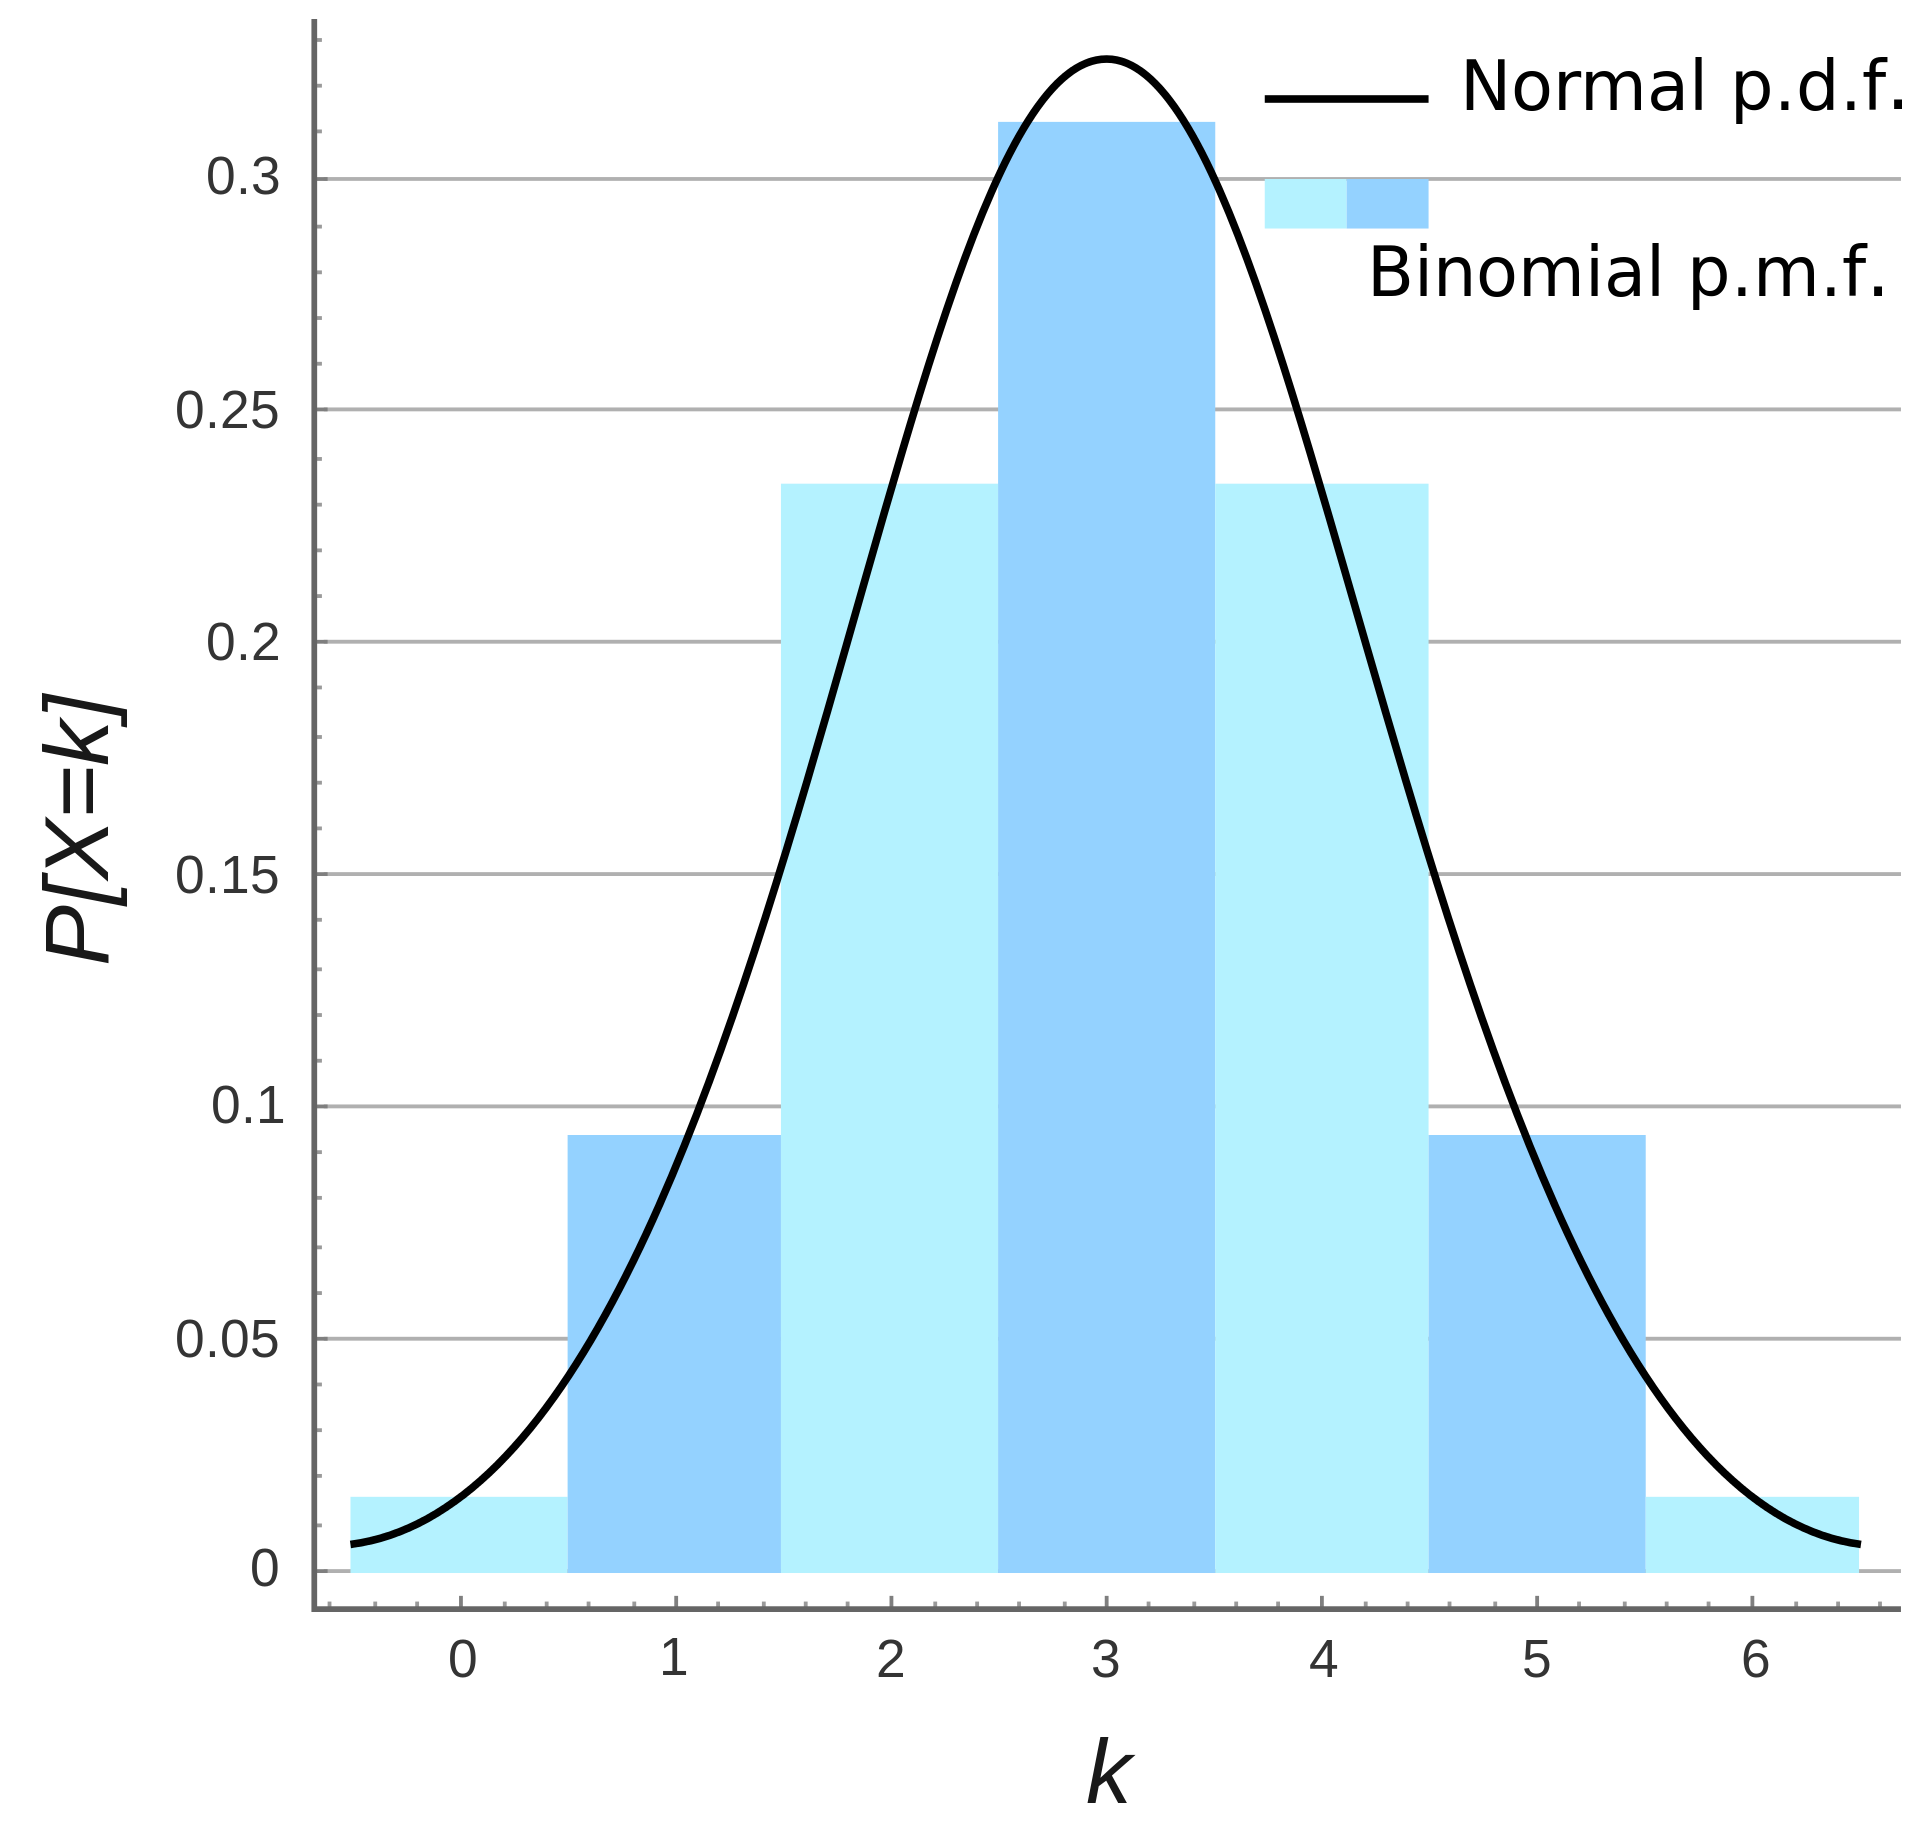
\includegraphics[width=7.5cm]{figures/binomial.png}
    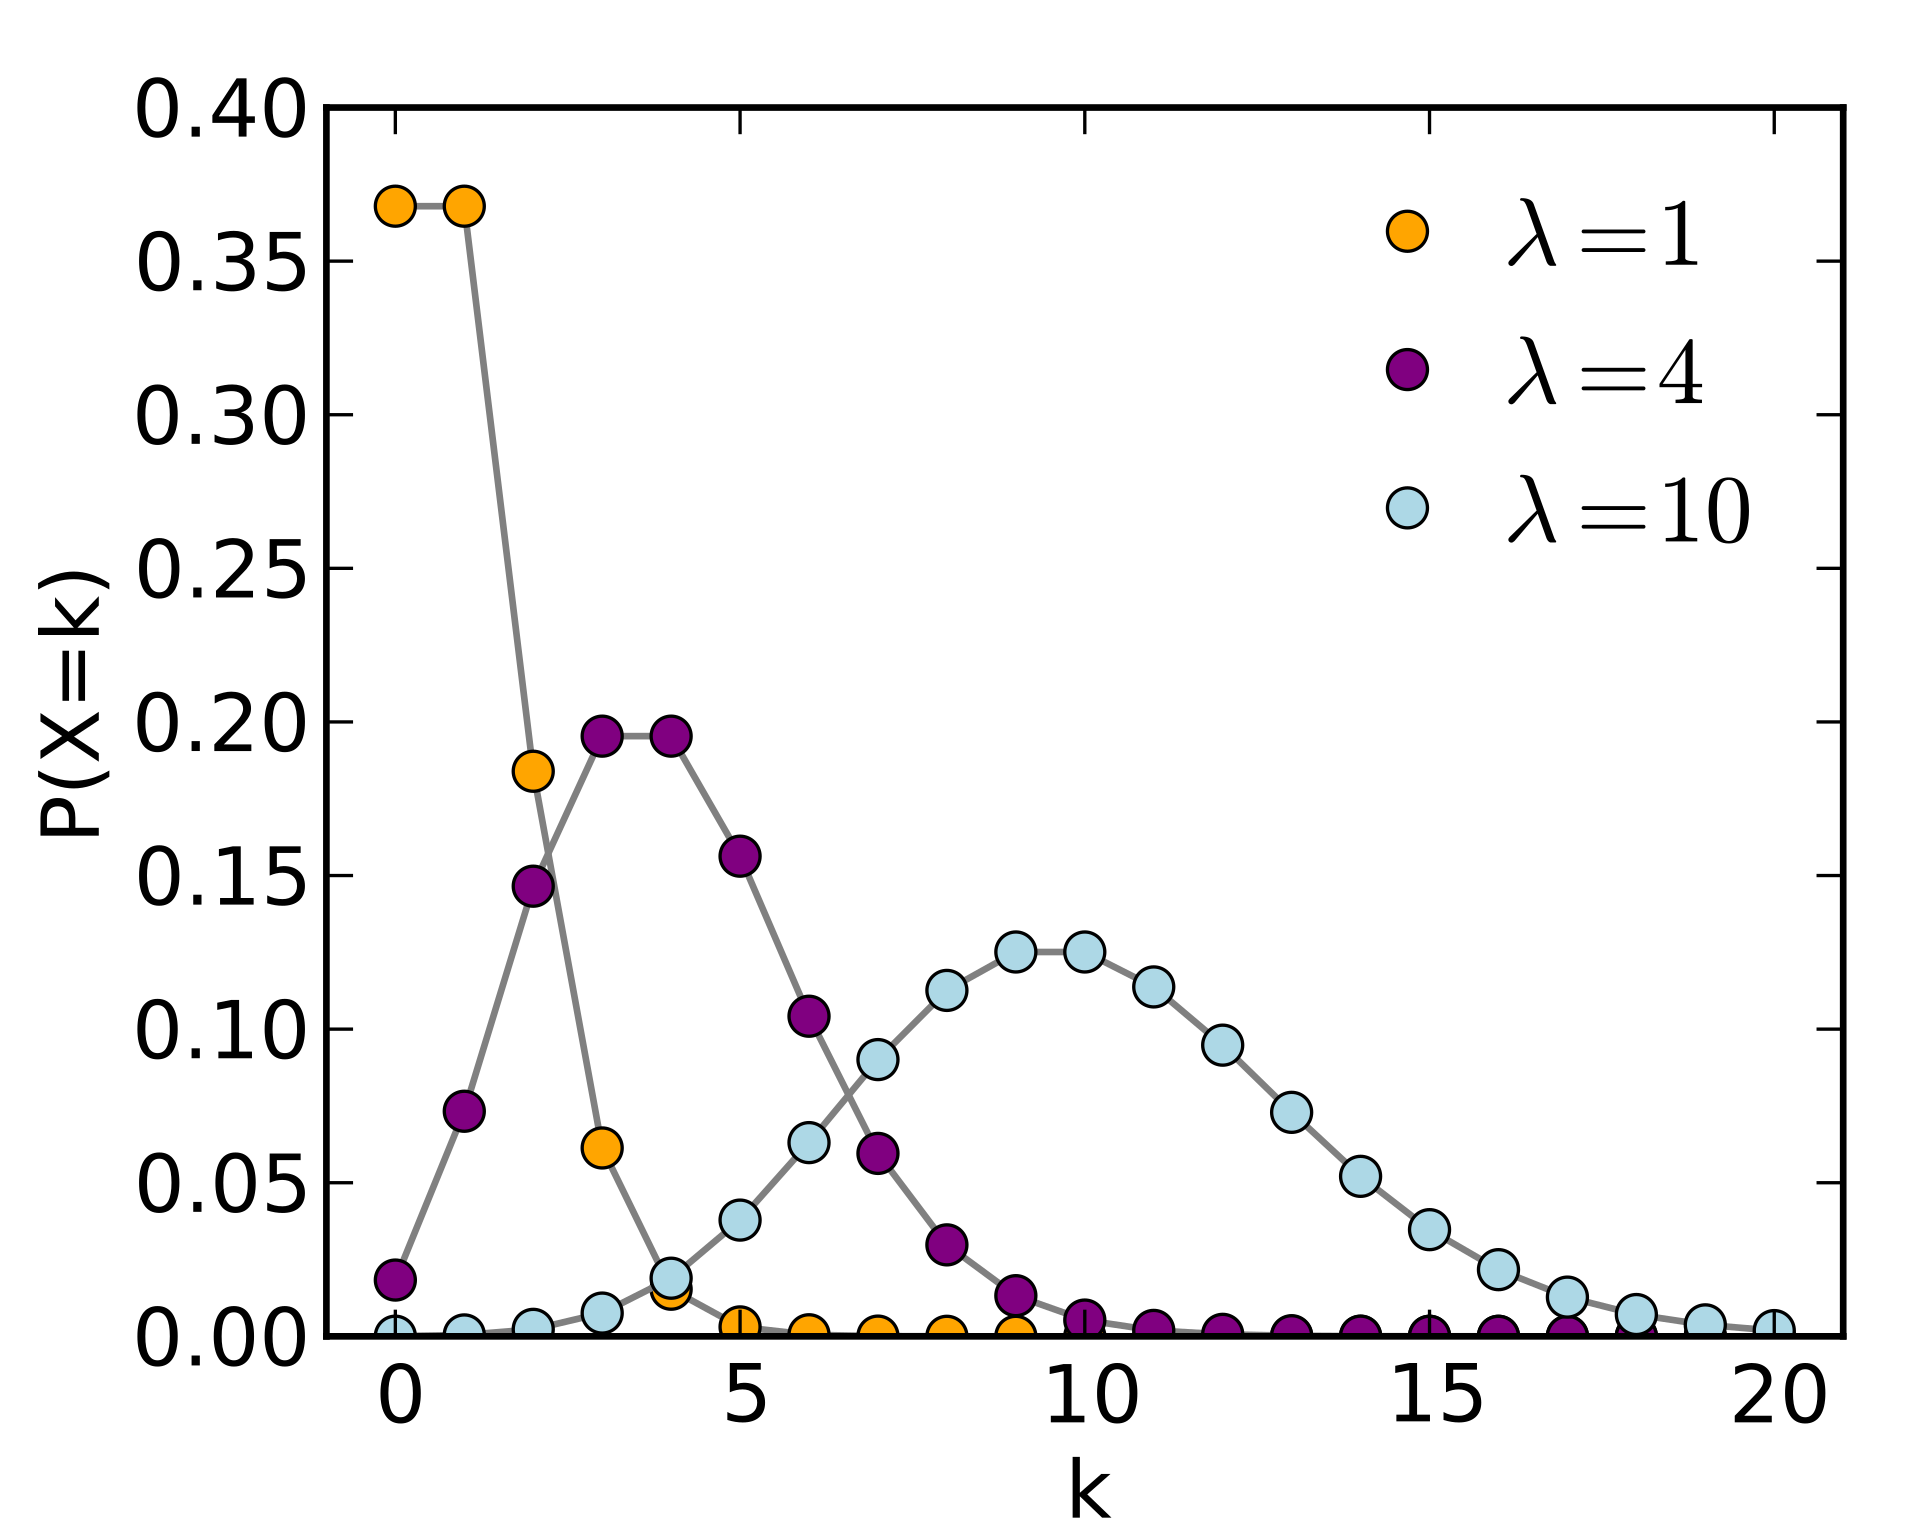
\includegraphics[width=7.5cm]{figures/poisson.png}
    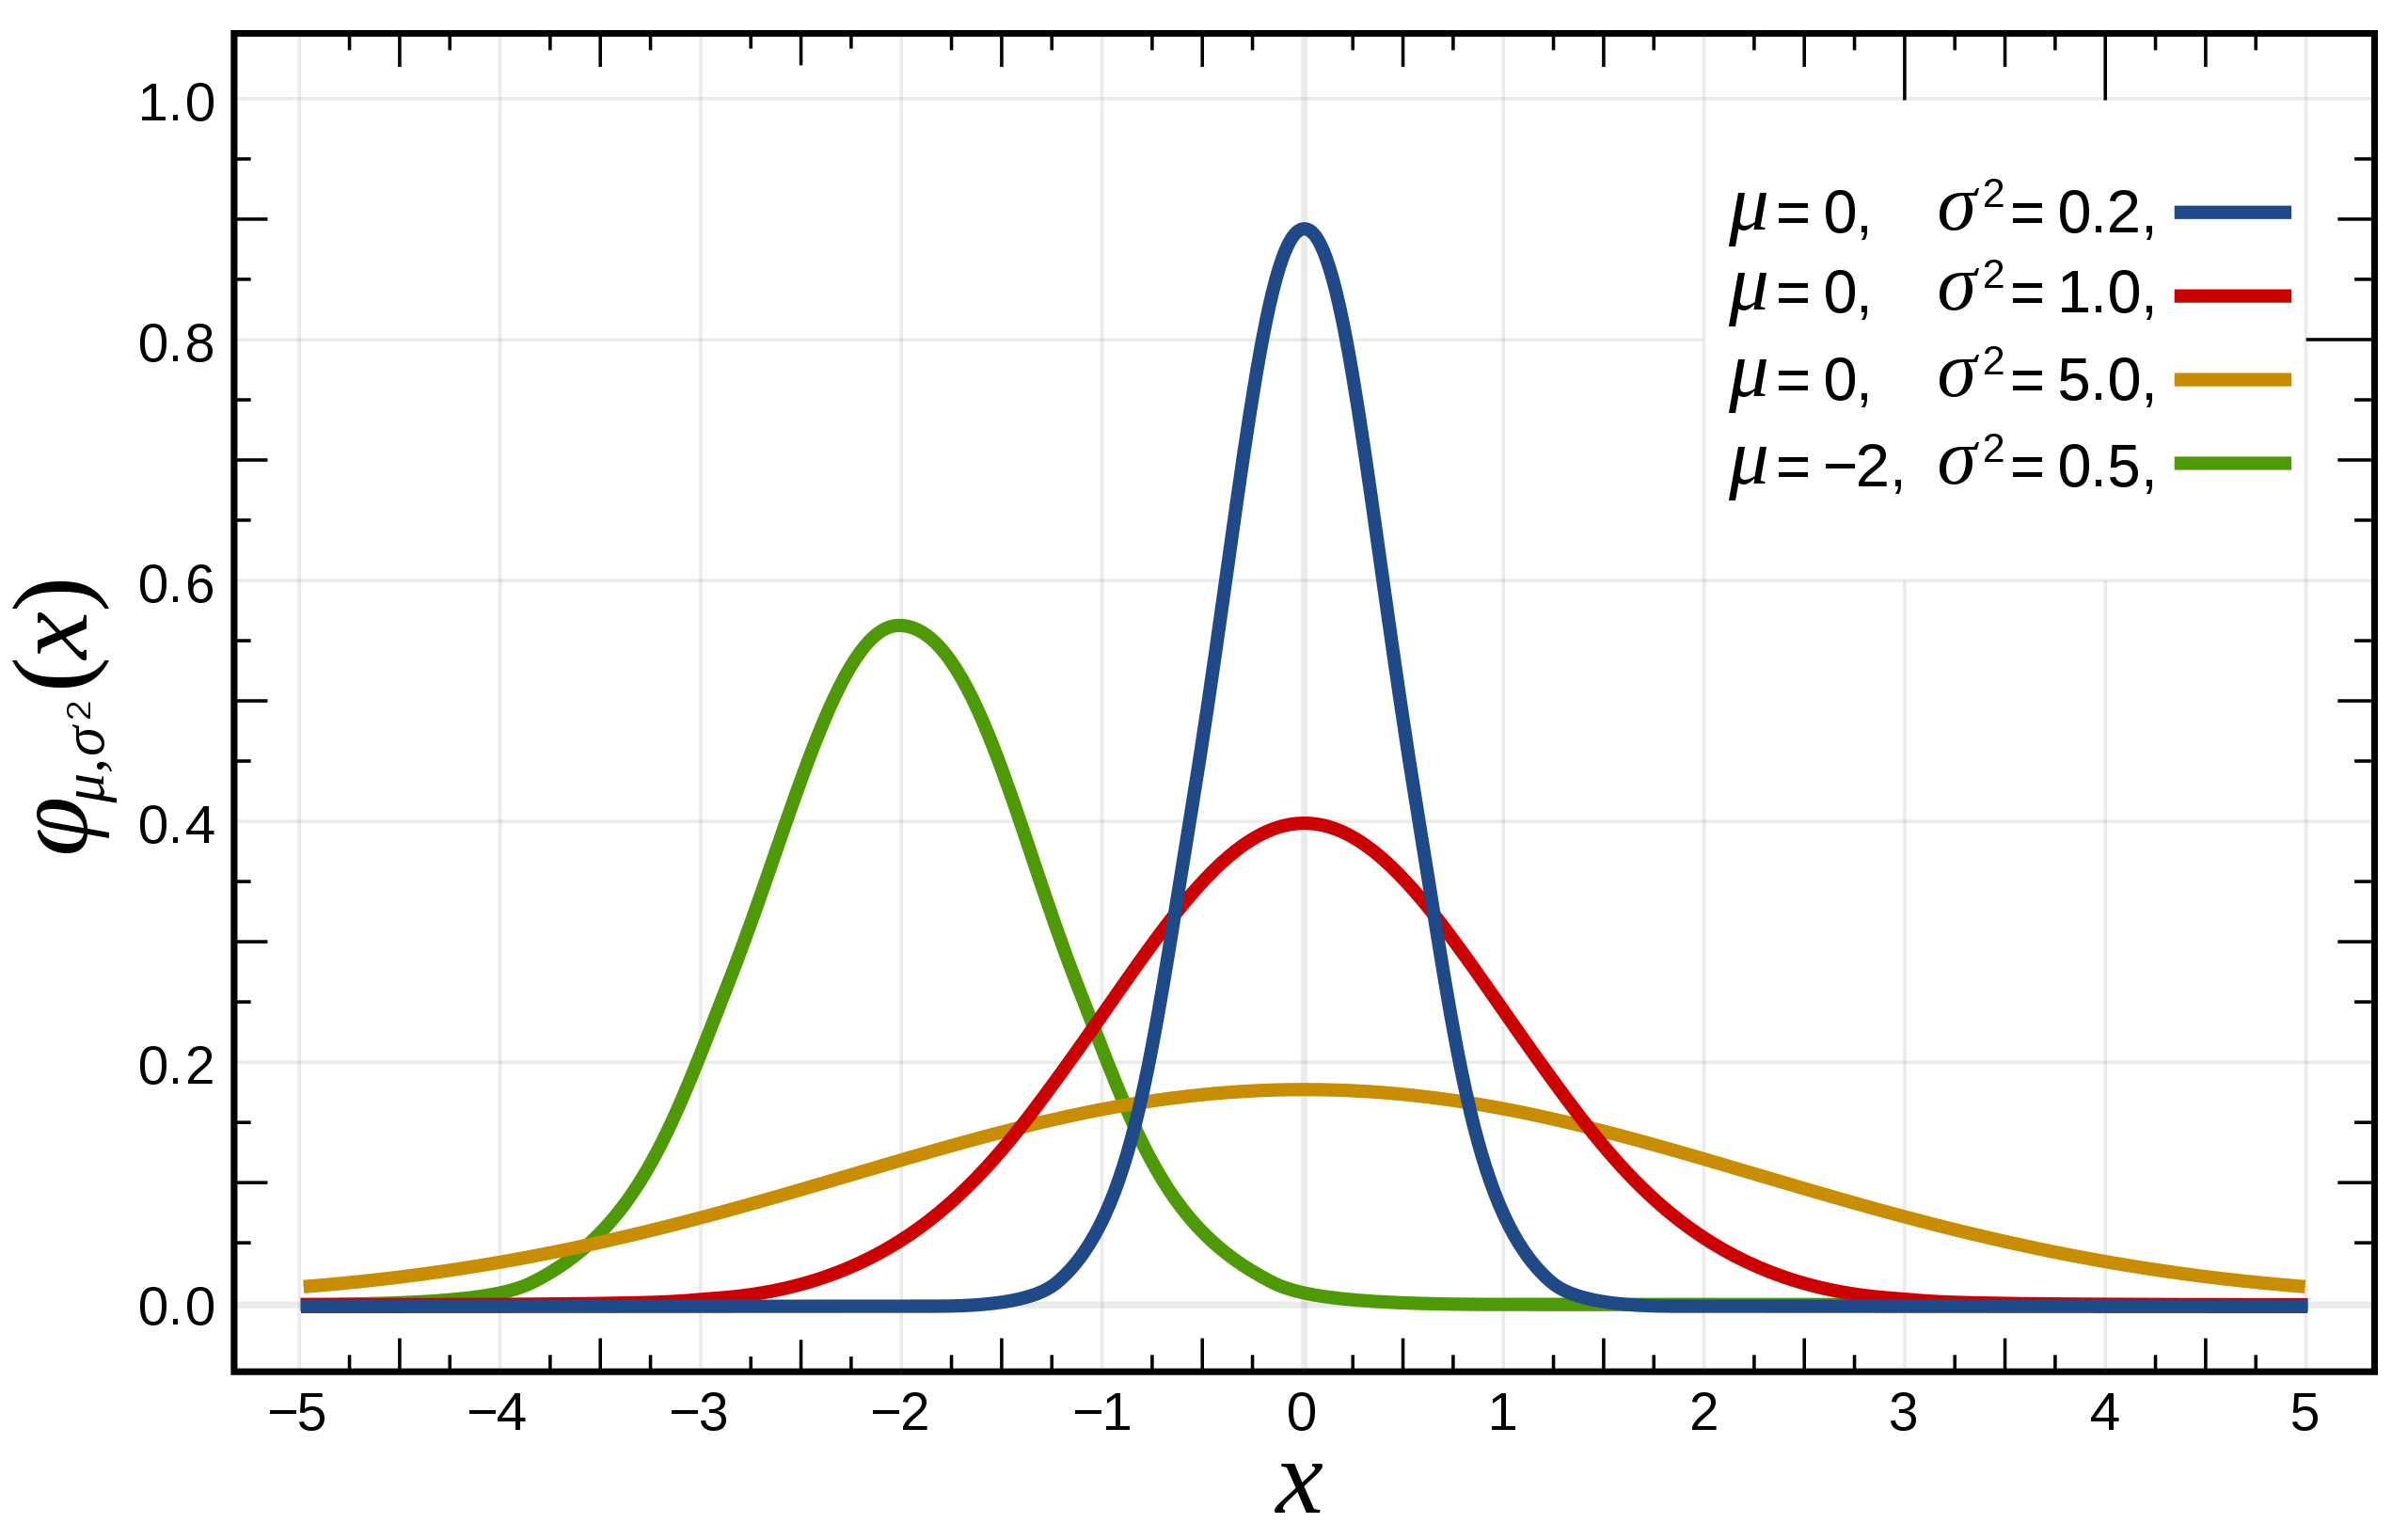
\includegraphics[width=7.5cm]{figures/gaussian.png}
    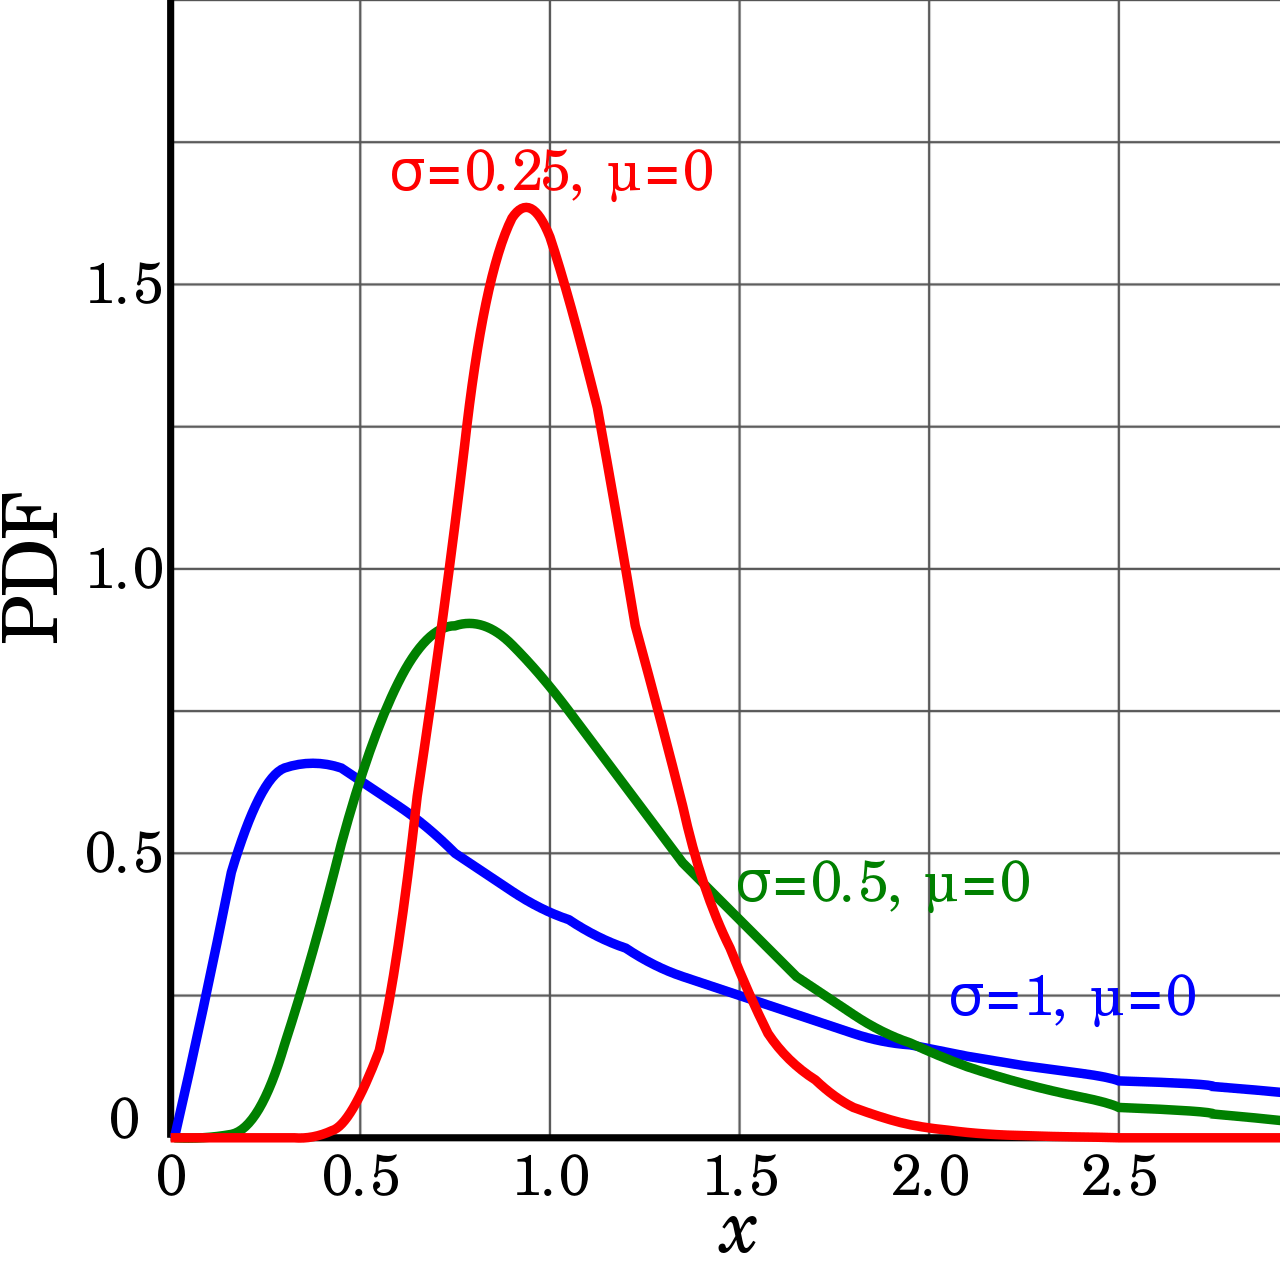
\includegraphics[width=7.5cm]{figures/log-normal.png}
    \caption{\footnotesize{\textbf{(Top left)}: Binomial distribution. \textbf{(Top right)}: Poisson distributions. \textbf{(Bottom left)}: Gaussian distributions. \textbf{(Bottom right)}: Log-normal distributions. Figures taken from Wikipedia.}}
    \label{fig:distributions}
\end{figure}

{\noindent}\textbf{Binomial distribution}: Suppose we toss a coin in the air and let it land. There is a $50\%$ probability that it will land heads up and a $50\%$ probability that it will land tails up. by this, we can that if we continue tossing a coin repeatedly, the fraction of times that it lands with heads up will asymptotically approach $1/2$, indicating that there was a probability of $1/2$ in doing so. For any given coin toss, the probability cannot determine whether or not it will lands heads up; it can only describe how we should expect a large number of tosses to be divided into these two possibilities.

{\noindent}Suppose we toss two coins at a time. There are now four different possible permutations of the way in which they can land: both heads up, both tails up, and two mixtures of heads and tails depending on which one is heads up. Because each of these permutations is equally probable, the probability for any choice of them is $1/4$ or $25\%$. To find the probability for obtaining a particular mixture of heads and tails, without differentiating between the two kinds of mixtures, we must add the probabilities corresponding to each possible kind. Thus, the total probability of finding either heads up and the other tails up is $1/2$. Note that the sum of the probabilities for all possibilities ($1/4+1/4+1/4+1/4$) is always equal to $1$ because \textit{something} is bound to happen.

{\noindent}Let us extrapolate these ideas to the general case. Suppose we toss $n$ coins into the air, where $n$ is some integer. Alternatively, suppose that we toss one coin $n$ times. What is the probability that exactly $x$ of these coins will land heads up, without distinguishing which of the coins actually belongs to which group? We can consider the probability $P(x;n)$ to be a function of the number of coins tossed $n$ and of the number of coins that land heads up $x$. For a given experiment in which $n$ coins are tossed, this probability $P(x;n)$ will vary as a function of $x$. Of course, $x$ must be an integer for any physical experiment, but we can consider the probability to be smoothly varying with $x$ as a continuous variable for mathematical purposes.

{\noindent}\textit{Permutations and combinations}: If $n$ coins are tossed, there are $2^n$ different possible ways in which they can land. This follows from the fact that the first coin has two possible orientations, for each of these the second coin also has two such orientations, for each of these the third coin also has two, and so on. Because each of these possibilities is equally probable, the probability for any one of these possibilities to occur at any toss of $n$ coins has to be $1/2^n$.

{\noindent}How many of these possibilities will contribute to our observation of $x$ coins with heads up? Imagine two boxes, one labeled ``heads'' and divided into $x$ slots, and the other labeled ``tails''. We shall considered first the question of how many permutations of the coins result in the proper separation of $x$ in one box and $n-x$ in the other; then we shall consider the question of how many combinations of these permutations should be considered different from each other.

{\noindent}In order to enumerate the number of \textbf{permutations} $Pm(n,x)$, let us pick up the coins one at a time from the collection of $n$ coins and put $x$ of them into the ``heads'' box. We have a choice of $n$ coins for the first one we pick up. For our second selection, we can choose from the remaining $n-1$ coins. The range of choice is diminished until the last selection of the $x$th coin can be made from only $n-x+1$ remaining coins. The total number of choices for coins to fill the $x$ slots in the ``heads'' box is the product of the numbers of individual choices:

\begin{align*}
    Pm(n,x) = n(n-1)(n-2) \cdot\cdot\cdot (n-x+2)(n-x+1).
\end{align*}

{\noindent}This expansion can be expressed more easily in terms of factorials:

\begin{align*}
    Pm(n,x) &= \frac{n!}{(n-x)!} ~ [{\rm dimensionless}].
\end{align*}

{\noindent}So far we have calculated the number of permutations $Pm(n,x)$ that will yield $x$ coins in the ``heads'' box and $n-x$ coins in the ``tails'' box, with the provision that we have identified which coin was places in the ``heads'' box first, which was placed in the second, and so on. That is, we have \textit{ordered} the $x$ coins in the ``heads'' box. In our computation of $2^n$ different possible permutations of the $n$ coins, we are only interested in which coins landed heads up or heads down, not which landed first. Therefore, we must consider contributions different only if there are different coins in the two boxes, not if the $x$ coins within the ``heads'' box are permuted into different time orderings.

{\noindent}The number of different \textbf{combinations} $C(n,x)$ of the permutations in the preceding enumeration results from combining the $x!$ different ways in which $x$ coins in the ``heads'' box can be permuted within the box. For ever $x!$ permutations, there will be only one new combination. Thus, the number of different combinations $C(n,x)$ is the number of permutations $Pm(n,x)$ divided by the degeneracy factor $x!$ of the permutations:

\begin{align*}
    C(n,x) = \frac{Pm(n,x)}{x!} = \frac{n!}{x!(n-x)!} = \binom{n}{x} ~ [{\rm dimensionless}]
\end{align*}

{\noindent}where $q=1-p$. The name for the binomial distribution comes from the fact that the coefficients $P_B(x;n,p)$ are closely related to the binomial theorem for the expansion of a power of a sum. According to the \textbf{binomial theorem},

\begin{align*}
    (p+q)^n = \sum _{x=0}^n \left[ \binom{n}{x}p^xq^{n-x} \right] ~ [{\rm dimensionless}].
\end{align*}

{\noindent}This is the number of different possible combinations of $n$ items taken $x$ at a time, commonly referred to as $\binom{n}{x}$ or ``$n$ over $x$''.

{\noindent}\textit{Probability}: The probability $P(x;n)$ that we should observe $x$ coins with heads up and $n-x$ with tails up is the product of different combinations $C(n,x)$ that contribute to that set of observations multiplied by the probability for each of the combinations to occur, which we have found to be $(1/2)^n$.

{\noindent}Actually, we should separate the probability for each combination into two parts: one part is the probability $p^x=(1/2)^x$ for $x$ coins to be heads up; the other part is the probability $q^{n-x} = (1-1/2)^{n-x} = (1/2)^{n-x}$ for the other $n-x$ coins to be tails up. For symmetrical coins, the product of these two parts $p^xq^{n-x}=(1/2)^n$ is the probability of the combination with $x$ coins heads up and $n-x$ coins tails up. In the general case, the probability $p$ of success for each item is not equal in magnitude to the probability $q=1-p$ for failure. For example, when tossing a die, the probability that a particular number will show up is $p=1/6$, while the probability of it now showing is $q=1-1/6=5/6$ so that $p^xq^{n-x}=(1/6)^x\times(5/6)^n$.

{\noindent}With these definitions of $p$ and $q$, the probability $P_B(x;n,p)$ for observing $x$ of the $n$ items to be in the state with probability $p$ is given by the \textbf{binomial distribution}:

\begin{align*}
    P_B(x;n,p) = \binom{n}{x}p^xq^{n-x} = \frac{n!}{x!(n-x)!}p^x(1-p)^{n-x} ~ [{\rm dimensionless}].
\end{align*}

{\noindent}Figure \ref{fig:distributions} (top left) shows an example binomial distribution.

{\noindent}\textbf{Poisson distribution}: The Poisson distribution represents an approximation to the binomial distribution for the special case where the average number of successes is much smaller than the possible number; that is, when $\mu\ll n$ because $p\ll1$. For such experiments the binomial distribution correctly describes the probability $P_B(x;n,p)$ of observing $x$ events per unit time interval out of $n$ possible events, each of which has a probability $p$ of occurring, but the large number of $n$ possible events makes exact evaluation from the binomial distribution impractical. Furthermore, neither the number $n$ of possible events nor the probability $p$ for each is usually known. What may be known instead is the average number of events $\mu$ expected in each time interval or its estimate $\bar{x}$. The Poisson distribution provides an analytical form appropriate to such investigations that describes the probability distribution in terms of just the variable $x$ and the parameter $\mu$. 

{\noindent}Let us consider the binomial distribution in the limiting case of $p\ll1$. We are interested in its behaviour as $n$ becomes infinitely large while the mean $\mu=np$ remains constant. The equation for the probability function of the binomial distribution can be written as

\begin{align*}
    P_B(x;n,p) = \frac{1}{x!} \frac{n!}{(n-x)!} p^x(1-p)^{-x}(1-p)^n ~ [{\rm function}].
\end{align*}

{\noindent}If we expand the second factor,

\begin{align*}
    \frac{n!}{(n-x)!} = n(n-1)(n-2) \cdot\cdot\cdot (n-x-2)(n-x-1) ~ [{\rm function}]
\end{align*}

{\noindent}we can consider it to be the product of $x$ individual factors, each of which is very nearly equal to $n$ because $x\ll n$ in the region of interest. The second factor in $P_B(x;n,p)$ above thus asymptotically approaches $n^x$. The product of the second and third factors then becomes $(np)^x=\mu^x$. The fourth factor is approximately equal to $(1+px)$ which tends to $1$ as $p$ tends to $0$.

{\noindent}The last factor can be rearranged by substituting $\mu/p$ for $n$ and expanding the expression to show that it asymptotically approaches $e^{-\mu}$:

\begin{align*}
    \lim_{p\rightarrow0}(1-p)^x = \lim_{p\rightarrow0} [(1-p)^{1/p}]^\mu = \left(\frac{1}{e}\right)^\mu = e^{-\mu} ~ [{\rm function}].
\end{align*}

{\noindent}Combining these approximation, we find that the binomial distribution probability function $P_B(x;n,p)$ asymptotically approaches the \textbf{Poisson distribution} $P_B(x;\mu)$ as $p$ approaches $0$:

\begin{align*}
    \lim_{p\rightarrow0}P_B(x;n,p) = P_P(x;\mu) \equiv \frac{\mu^x}{x!}e^{-\mu} ~ [{\rm function}].
\end{align*}

{\noindent}Because this distribution is an approximation to the binomial distribution for $p\ll1$, the distribution is asymmetric about its mean $\mu$. Note that $P_P(x;\mu)$ does not become $0$ for $x=0$ and is not defined for negative values of $x$. This restriction is not troublesome for counting experiments because the number of counts per unit time interval can never be negative.

{\noindent}\textit{Derivation}: The Poisson distribution can also be derived for the case where the number of events observed is small compared to the total possible number of events. Assume that the average rate at which events of interest occur is constant over a given interval of time and that event occurrences are randomly distributed over that interval. Then, the probability ${\rm d}P$ of observing no events in a time interval ${\rm d}t$ is given by

\begin{align*}
    {\rm d}P(0;t\tau) = -P(0;t,\tau)\frac{{\rm d}t}{\tau} ~ [{\rm function}]
\end{align*}

{\noindent}where $P(x;t,\tau)$ is the probability of observing $x$ events in the time interval ${\rm d}t$, $\tau$ is a constant proportionality factor that is associated with the mean time between events, and the minus sign accounts for the fact that increasing the differential time interval ${\rm d}t$ decreases the probability proportionality. Integrating this equation yields the probability of observing no events within a time $t$ to be

\begin{align*}
    P(0;t,\tau) = P_0e^{-t/\tau} ~ [{\rm function}]
\end{align*}

{\noindent}where $P_0$, the constant of integration, is equal to $1$ because $P(0;t,\tau)=1$ at $t=0$.

{\noindent}The probability $P(x;t,\tau)$ for observing $x$ events in the time interval $\tau$ can be evaluated by integrating the differential probability

\begin{align*}
    {\rm d}^xP(x;t,\tau) = \frac{e^{-t/\tau}}{x!} \prod_{i=1}^x \frac{{\rm d}t_i}{\tau} ~ [{\rm function}]
\end{align*}

{\noindent}which is the product of the probabilities of observing each events in a different interval ${\rm d}t_i$ and the probability $e^{-t/\tau}$ of not observing any other events in the remaining time. The factor of $x!$ in the denominator compensates for the ordering implicit in the probabilities ${\rm d}P_i(l,t,\tau)$.

{\noindent}Thus, the probability of observing $x$ events in the time interval $t$ is obtained by integration

\begin{align*}
    P_P(x;\mu) = P(x;t,\tau) = \frac{e^{-t/\tau}}{x!} \left(\frac{t}{\tau}\right)^x ~ [{\rm function}]
\end{align*}

{\noindent}or

\begin{align*}
    P_P(x;\mu) = \frac{\mu^x}{x!} e^{-\mu} ~ [{\rm function}]
\end{align*}

{\noindent}which is the expression for the Poisson distribution, where $\mu=t/\tau$ is the average number of events observed in the time interval $t$. This equation represents a \textbf{normalized probability function}; that is, the sum of the function evaluated at each of the allowed values of the variable $x$ is unity:

\begin{align*}
    \sum_{x=0}^\infty P_P(x,\mu) = \sum_{x=0}^\infty \frac{\mu^x}{x!} e^{-\mu} = e^{-\mu} \sum_{x=0}^\infty \frac{\mu^x}{x!} = e^{-\mu}e^{\mu} = 1.
\end{align*}

{\noindent}\textit{Mean and standard deviation}: The Poisson distribution, like the binomial distribution, is a \textit{discrete} distribution. That is, it is only defined only at integral values of the variable $x$, although the parameter $\mu$is a positive, real number. The mean of the Poisson distribution is actually the parameter $\mu$ that appears in the probability function $P_P(x;\mu)$. To verify this, we can evaluate the expectation value $\langle x\rangle$ of $x$: 

\begin{align*}
    \langle x\rangle = \sum_{x=0}^\infty \left(x\frac{\mu^x}{x!}e^{-\mu}\right) = \mu e^{-\mu} \sum_{x=1}^\infty \frac{\mu^{x-1}}{(x-1)!} = \mu e^{-\mu} \sum_{y=0}^\infty \frac{\mu^y}{y!} = \mu.
\end{align*}

{\noindent}To find the standard deviation $\sigma$, the expectation value of the square of the deviations can be evaluated:

\begin{align*}
    \sigma^2 = \langle (x-\mu)^2 \rangle = \sum_{x=0}^\infty \left[ (x-\mu)^2\frac{\mu^x}{x!}e^{-\mu} \right] = \mu ~ [{\rm function}].
\end{align*}

{\noindent}Thus, the standard deviation $\sigma$ is is equal to the square root of the mean $\mu$ and the Poisson distribution has only a single parameter, $\mu$.

{\noindent}Computation of the Poisson distribution by

\begin{align*}
    P_P(x;\mu) = \frac{\mu^x}{x!} e^{-\mu} ~ [{\rm function}]
\end{align*}

{\noindent}can be limited by the factorial function in the denominator. The problem can be avoided by using logarithms or by using the recursive relations

\begin{align*}
    P(0;\mu)=e^{-\mu}, ~~~ P(x;\mu)=\frac{\mu}{x}(x-1;\mu).
\end{align*}

{\noindent}This form has the disadvantage that, in order to calculate the function for particular values of $x$ and $\mu$, the function must be calculated at all lower values of $x$ as well. However, if the function is to be summed from $x=0$ to some upper limit to obtain the summed probability or to generate the distribution for a Monte Carlo calculation, the function must be calculated at all lower values of $x$ anyway.

{\noindent}\textit{Summed probability}: We may want to know the probability of obtaining a sample value of $x$ between limits $x_1$ and $x_2$ from a Poisson distribution with mean $\mu$. This probability is obtained by summing the values of the function calculated at the integral values of $x$ between the two integral limits $x_1$ and $x_2$,

\begin{align*}
    S_P(x_1,x_2;\mu) = \sum_{x_1}^{x_2} P_P(x;\mu).
\end{align*}

{\noindent}More likely, we may want to find the probability of recording $n$ or more events in a given interval when the mean number of events is $\mu$. This is just the sum 

\begin{align*}
    S_P(n,\infty;\mu) = \sum_{x=n}^\infty P_P(x;\mu)= 1-\sum_{x=0}^{n-1} P_P(x;\mu) = 1-e^{-\mu} \sum_{x=0}^{n-1} \frac{\mu^x}{x!} ~ [{\rm function}].
\end{align*}

{\noindent}So, this distribution has the special property that the mean is equal to the variance.

{\noindent}The first four moments of the Poisson distribution are given by:

\begin{enumerate}
    \item ${\rm Mean} = \mu$
    \item ${\rm Variance} = \mu$
    \item ${\rm Skewness} = \mu$
    \item ${\rm Kurtosis} = 3\mu^2+\mu$.
\end{enumerate}

{\noindent}For large values of $\mu$, the probability sum may be approximated by an integral of the Gaussian function.

{\noindent}Figure \ref{fig:distributions} (top right) shows an example Poisson distribution.

{\noindent}\textit{Application}: A steady celestial source of constant luminosity produces on average a finite number of counts in a detector every second. The photons do not arrive with equal intervals. The average rate of arrival is controlled by a fixed probability of an event occur- ring in some fixed interval of time. There is some chance of an event occurring in every millisecond, but no certainty that the event will indeed arrive in any specific millisecond. This randomness leads to a variation in the number of counts detected in successive intervals.

{\noindent}\textbf{Gaussian (or normal error) distribution}: The Gaussian distribution is an approximation to the binomial distribution for the special limiting case where the number of possible different observations $n$ becomes infinitely large and the probability of success for each is finitely large so $np\gg1$. It is also the limiting case for the Poisson distribution as $\mu$ becomes large.

{\noindent}There are several derivations of the Gaussian distribution from first principles, none of them as convincing as the fact that the distribution is reasonable, that it has a fairly simple analytic form, and that it is accepted by convention and experimentation to be the most likely distribution for most experiments. In addition, it has the satisfying characteristic that the most probable estimate of the mean $\mu$ from a random sample of observations $x$ is the average of those observations $\bar{x}$.

{\noindent}\textit{Characteristics}: The Gaussian probability density is defined as

\begin{align*}
    p_G = \frac{1}{\sigma\sqrt{2\pi}}\exp \left[-\frac{1}{2} \left(\frac{x-\mu}{\sigma}\right)^2 \right] ~ [{\rm dimensionless}].
\end{align*}

{\noindent}This distribution is \textbf{symmetrical} and \textbf{mesokurtic}. It is a continuous function describing the probability of obtaining the value $x$ in a random observation from a parent distribution with parameters $\mu$ and $\sigma$, corresponding to the mean and standard deviation, respectively. Because the distribution is continuous, we must define an interval in which the value of the observation $x$ will fall. The probability density function is properly defined such that the probability that the value of a random observation ${\rm d}P_G(x;\mu,\sigma)$ will fall within an interval ${\rm d}x$ around $x$ is given by

\begin{align*}
    {\rm d}P_G(x;\mu,\sigma) = p_G(x;\mu,\sigma){rm d}x ~ [{\rm dimensionless}],
\end{align*}

{\noindent}considering ${\rm d}x$ to be an infinitesimal differential, and the probability density function to be normalized, so that

\begin{align*}
    \int\limits_{x=-\infty}^{x=\infty} {\rm d}P_G(x;\mu,\sigma) = \int\limits_{x=-\infty}^{x=\infty} p_G(x;\mu,\sigma){\rm d}x ~ [{\rm dimensionless}].
\end{align*}

{\noindent}The width of the curve is determined by the value of $\sigma$, such that for $x=\mu+\sigma$, the height of the curve is reduced to $e^{-1/2}$ of its value at the peak:

\begin{align*}
    p_G(x;\mu\pm\sigma,\sigma) = e^{-1/2}p_G(\mu;\mu,\sigma) ~ [{\rm dimensionless}].
\end{align*}

{\noindent}We can characterize a distribution by its \textbf{full-width at half maximum} (FWHM) $\Gamma$, often referred to as the \textbf{half-width}, defined as the range of $x$ between values at which the probability $p_G(x;\mu,\sigma)$ is half its maximum value:

\begin{align*}
    p_G(\mu\pm\frac{1}{2}\Gamma,\mu,\sigma) = \frac{1}{2}p_G(\mu;\mu,\sigma) ~ [{\rm function}].
\end{align*}

{\noindent}With this definition, we can determine from the Gaussian probability density $p_G$ that

\begin{align*}
    \Gamma=2\sqrt{2\ln2}\sigma \approx 2.354\sigma ~ [{\rm function}].
\end{align*}

{\noindent}Tangents drawn along a portion of steepest descent of the curve intersect the curve at the $e^{-1/2}$ points $x=\mu\pm\sigma$ and intersect the $x$ axis at the points $x=\mu\pm2\sigma$.

{\noindent}The first four moments of the Gaussian distribution are given by:

\begin{enumerate}
    \item ${\rm Mean} = \mu$
    \item ${\rm Variance} = \sigma^2$
    \item ${\rm Skewness} = 0$
    \item ${\rm Kurtosis} = 3\sigma^4$.
\end{enumerate}

{\noindent}Figure \ref{fig:distributions} (bottom left) shows an example Gaussian distribution.

{\noindent}Regardless of statistical considerations, there are a number of reasons why the normal distribution is much better known than the log-normal. A major one appears to be symmetry, one of the basic principles realized in nature as well as in our culture and thinking. Thus, probability distributions based on symmetry may have more inherent appeal than skewed ones. Two other reasons relate to simplicity. First, as Aitchison and Brown states, ``Man has found addition an easier operation than multiplication, and so it is not surprising that an additive law of errors was the first to be formulated.'' Second, the established, concise description of a normal sample is handy, well-known, and sufficient to represent the underlying distribution, which made it easier, until now, to handle normal distributions than to work with log-normal distributions. Another reason relates to the history of distributions: The normal distribution has been known and applied more than twice as long as its log-normal counterpart. Finally, the very notion of ``normal'' conjures more positive associations for non-statisticians than does ``log-normal.'' For all of these reasons, the normal or Gaussian distribution is far more familiar than the log-normal distribution is to most people.

{\noindent}\textit{Application}: Gaussian function approximates the shapes of many observables in astronomy, such as the profiles of seeing disks, the width of spectral lines and the distribution of noise in radio receivers. In error analysis, the Gaussian distribution is often used to determine the significance of a measurement is the presence of noise.

{\noindent}\textbf{Log-normal distribution}: Many measurements show a more or less skewed distribution. Skewed distributions are particularly common when mean values are low, variance large, and values cannot be negative. Such skewed distributions often closely fit the log-normal distribution. What is the difference between normal and log-normal variability? Both forms of variability are based on a variety of forces acting independently of one another. A major difference, however, is that the effects can be additive or multiplicative, thus leading to normal or log-normal distributions, respectively.

{\noindent}Some basic principles of additive and multiplicative effects can easily be demonstrated with the help of two ordinary dice with sides numbered from $1$ to $6$. Adding the two numbers, which is the principle of most games, leads to values of $2$ to $12$, with a mean of $7$, and a symmetrical frequency distribution. The total range can be described as $7$ plus or minus $5$ (i.e., $7\pm5$); note that in this case, $5$ is not the standard deviation. Multiplying the two numbers, however, leads to values between $1$ and $36$ with a highly skewed distribution. The total variability can be described as $6$ multiplied or divided by $6$. In this case, the symmetry has moved to the multiplicative level.

{\noindent}Although these examples are neither normal nor log-normal distributions, they do clearly indicate that additive and multiplicative effects give rise to different distributions. Thus, we cannot describe both types of distributions in the same way. Unfortunately, however, common belief has it that quantitative variability is generally bell shaped and symmetrical. The current practice in science is to use symmetrical error bars in graphs to indicate standard deviations or errors, and the sign $\pm$ to summarize data, even though the data or underlying principles may suggest skewed distributions.

{\noindent}Log-normal distributions are usually characterized in terms of the log-transformed variable, using as parameters the expected value, or mean, of its distribution and its standard deviation. This characterization can be advantageous as, by definition, log-normal distributions are symmetrical again at the log level. Unfortunately, the widespread aversion to statistics becomes even more pronounced as soon as logarithms are involved. This may be the major reason that the log-normal distributions are so little understood in general, which leads to frequent misunderstandings and errors. Plotting the data can help, but graphs are difficult to communicate orally. In short, current ways of handling log-normal distributions are often unwieldy. To get an idea of a sample, most people prefer to think in terms of the original rather than the log-transformed data. This conception is indeed feasible and advisable for log-normal data too, because the familiar properties of the normal distribution have their analogies in the log-normal distribution.

{\noindent}A set of observations $x$ is said to have a log-normal distribution if $\ln(x)$ or $\log(x)$ is \textit{normally distributed}. Here, the range of $x$ is exclusively positive (i.e., $0<x<\infty$) and skewed towards the left. It is also known as a \textbf{Galton distribution}. A variable might be modelled as log-normal if it can be thought of as the multiplicative product of many independent random variables each of which is positive. This distribution is \textbf{positively skewed} and \textbf{leptokurtic}.

{\noindent}The log-normal probability distribution is defined as

\begin{align*}
    p_L = \frac{1}{x\sqrt{2\pi\sigma^2}} \exp \left[-\frac{(\ln x-\mu)^2}{2\sigma^2}\right] ~ [{\rm dimensionless}]
\end{align*}

{\noindent}which has the following descriptors:

\begin{enumerate}
    \item ${\rm Mean} = e^{\mu+\sigma^2/2}$
    \item ${\rm Median} = e^\mu$
    \item ${\rm Mode} = e^{\mu-\sigma^2}$
    \item ${\rm Variance} = (e^{\sigma^2}-1)e^{2\mu+\sigma^2}$
    \item ${\rm Skewness} = (e^{\sigma^2}+2)\sqrt{e^{\sigma^2}-1}$.
\end{enumerate}

{\noindent}Figure \ref{fig:distributions} (bottom right) shows an example log-normal distribution.

{\noindent}\textit{Application}:

{\noindent}\textbf{Summary}:

\begin{itemize}
    \item \textbf{Binomial distribution}: describes the probability of observing $x$ successes out of $n$ tries when the probability for success in each try is $p$:
\end{itemize}

\begin{align*}
    p_B(x;n,p) = \binom{n}{x}p^xq^{n-x} &= \frac{n!}{x!(n-x)!}p^x(1-p)^{n-x} \\
    \mu=np ~~~~~~ \sigma^2&=np(1-p)
\end{align*}

\begin{itemize}
    \item \textbf{Poisson distribution}: Limiting case of the binomial distribution for large $n$ and constant $\mu$; appropriate for describing small samples from large populations:
\end{itemize}

\begin{align*}
    p_P(x;\mu) = \frac{\mu^x}{x!}e^{-\mu}  ~~~ \sigma^2=\mu
\end{align*}

\begin{itemize}
    \item \textbf{Gaussian distribution}: Limiting case of the binomial distribution for large $n$ and finite $\mu$; appropriate for smooth symmetric distributions:
\end{itemize}

\begin{align*}
    p_G(x;\mu,\sigma) = \frac{1}{\sigma\sqrt{2\pi}} \exp \left[-\frac{1}{2}\left(\frac{x-\mu}{\sigma}\right)^2\right] \\
    {\rm (FWHM)}\,\Gamma=2\sqrt{2\ln2}\sigma \approx 2.354\sigma
\end{align*}

\subsubsection{Follow-up Questions}

\begin{itemize}
    \item What sort of noise do you expect for these?
    \item What extra sources of noise can you get from a CCD?
    \item Where does the noise come from, and what does the variance/standard deviation actually tell you?
    \item What property of the Gaussian distribution makes it particularly useful? (i.e., Central limit theorem.)
    \item How do we get a log-normal distribution?
    \item Why do we quote n-sigma probabilities and confidence levels with a Gaussian assumption when the actual probability distribution might not be Gaussian?
    \item If I'm doing a cosmological survey and I say I assume a Poisson distribution for radio galaxy sources and a Gaussian distribution for dust sources, why would I use two different distributions?
\end{itemize}

% --------------------------------------------------------------
%               16. 
% --------------------------------------------------------------

\newpage
\subsection{Question 16}

You are trying to determine a flux from a CCD image using aperture photometry, measuring source(+sky) within a 5-pixel radius, and sky within a 20-25 pixel annulus. Assume you find 10000 electrons inside the aperture and 8100 electrons in the sky region, and that the flux calibration is good to 1\%. What is the fractional precision of your measurement? (Ignore read noise.) More generally, describe how you propagate uncertainties, what assumptions you implicitly make, and how you might estimate errors if these assumptions do not hold.

\subsubsection{Short answer}

Answer.

\subsubsection{Additional context}

Additional context.

% --------------------------------------------------------------
%               17. 
% --------------------------------------------------------------

\newpage
\subsection{Question 17}

Suppose you measure the brightness of a star ten times (in a regime where source- noise dominates. (1) How do you calculate the mean, median, and mode and standard deviation? (2) How can you tell if any points are outliers? Say some points are outliers, what do you do now (i.e., how does this impact the calculation of the quantities in part 1)?

\subsubsection{Short answer}

Answer.

\subsubsection{Additional context}

Additional context.

\subsubsection{Follow-up Questions}

\begin{itemize}
    \item How would you go about fitting a model to your data? (i.e., Bayesian approach.)
    \item Why is using a gaussian generally a good choice?
\end{itemize}

% --------------------------------------------------------------
%               18. 
% --------------------------------------------------------------

\newpage
\subsection{Question 18}

Suppose you do an imaging search for binaries for a sample of 50 stars, and that you find companions in 20 cases. What binary fraction do you infer? Suppose a binary- star fraction of 50\% had been found previously for another sample (which was much larger, so you can ignore its uncertainty). Determine the likelihood that your result is consistent with that fraction.

\subsubsection{Short answer}

Answer.

\subsubsection{Additional context}

Additional context.

% --------------------------------------------------------------
%               19. 
% --------------------------------------------------------------

\newpage
\subsection{Question 19}

What are the primary wavelength bands at which searches for gravitational waves are conducted? What techniques are used to search in each band? What are the sources of gravitational waves in each band? What can we learn from detections (or non-detections)?

\subsubsection{Short answer}

Answer.

\subsubsection{Additional context}

In 1916, the year after the final formulation of the field equations of general relativity, Albert Einstein predicted the existence of gravitational waves. He found that the linearized weak-field equations had wave solutions: transverse waves of spatial strain that travel at the speed of light, generated by time variations of the mass quadrupole moment of the source. Einstein understood that gravitational-wave amplitudes would be remarkably small; moreover, until the Chapel Hill conference in 1957 there was significant debate about the physical reality of gravitational waves.

{\noindent}Also in 1916, Schwarzschild published a solution for the field equations that was later understood to describe a black hole, and in 1963 Kerr generalized the solution to rotating black holes. Starting in the 1970s theoretical work led to the understanding of black hole quasi-normal modes, and in the 1990s higher-order post-Newtonian calculations preceded extensive analytical studies of relativistic two-body dynamics. These advances, together with numerical relativity breakthroughs in the past decade, have enabled modeling of binary black hole mergers and accurate predictions of their gravitational waveforms. While numerous black hole candidates have now been identified through EM observations, black hole mergers have not previously been observed.

{\noindent}The discovery of the binary pulsar system PSR B1913+16 by Hulse and Taylor in 1975 and subsequent observations of its energy loss by Taylor and Weisberg in 1982 demonstrated the existence of gravitational waves. This discovery, along with emerging astrophysical understanding, led to the recognition that direct observations of the amplitude and phase of gravitational waves would enable studies of additional relativistic systems and provide new tests of general relativity, especially in the dynamic strong-field regime.

{\noindent}Experiments to detect gravitational waves began with Weber and his resonant mass detectors in the 1960s, followed by an international network of cryogenic resonant detectors. Interferometric detectors were first suggested in the early 1960s and the 1970s. A study of the noise and performance of such detectors, and further concepts to improve them, led to proposals for long-baseline broadband laser interferometers with the potential for significantly increased sensitivity. By the early 2000s, a set of initial detectors was completed, including TAMA 300 in Japan, GEO 600 in Germany, the Laser Interferometer Gravitational-Wave Observatory (LIGO) in the United States, and Virgo in Italy. Combinations of these detectors made joint observations from 2002 through 2011, setting upper limits on a variety of gravitational-wave sources while evolving into a global network. In 2015, Advanced LIGO became the first of a significantly more sensitive network of advanced detectors to begin observations.

{\noindent}A century after the fundamental predictions of Einstein and Schwarzschild, the first direct detection of gravitational waves and the first direct observation of a binary black hole system merging to form a single black hole was discovered in January of 2016. This discovery provided unique access to the properties of space-time in the strong-field, high-velocity regime and confirmed predictions of general relativity for the nonlinear dynamics of highly disturbed black holes.

{\noindent}There is an enormous difference between gravitational waves and the EM waves on which our present knowledge of the universe is based:

\begin{itemize}
    \item EM waves are oscillations of the EM field that propagate through spacetime; gravitational waves are oscillations of the ``fabric'' of spacetime itself.
    \item Astronomical EM waves are almost always incoherent superpositions of emission from individual electrons, atoms, or molecules. Cosmic gravitational waves are produced by coherent, bulk motions of huge amounts of mass-energy -- either material mass or the energy of vibrating, nonlinear spacetime curvature.
    \item Since the wavelengths of EM waves are small compared to their sources (gas clouds, stellar atmospheres, accretion disks, etc.), from the waves we can make pictures of the sources. The wavelengths of cosmic gravitational waves are comparable to or larger than their coherent, bulk-moving sources, so we cannot make pictures from them. Instead, the gravitational waves are like sound; they carry, in two independent waveforms, a stereophonic, symphony-like description of their sources.
    \item EM waves are easily absorbed, scattered, and dispersed by matter. Gravitational waves travel nearly unscathed through all forms and amounts of intervening matter.
    \item Astronomical EM waves have frequencies that begin at $\nu=10^7\,{\rm Hz}$ and extend on upward by roughly $20$ orders of magnitude. Astronomical gravitational waves should begin at $\nu\sim10^4\,{\rm Hz}$ ($1000$-fold lower than the lowest-frequency astronomical EM waves) and should extend on downward from there by roughly $20$ orders of magnitude.
\end{itemize}

{\noindent}These enormous differences make it likely that:

\begin{itemize}
    \item The information brought to us by gravitational waves will be very different from (almost ``orthogonal to'') that carried by EM waves; gravitational waves will show us details of the bulk motion of dense concentrations of energy, whereas electromagnetic waves show us the thermodynamic state of optically thin concentrations of matter.
    \item Most (but not all) gravitational-wave sources that our instruments detect will not be seen electromagnetically, and conversely, most objects observed electromagnetically will never be seen gravitationally. Typical EM sources are stellar atmospheres, accretion disks, and clouds of interstellar gas -- none of which emit significant gravitational waves, while typical gravitational-wave sources are the cores of supernova (which are hidden from electromagnetic view by dense layers of surrounding stellar gas), and colliding black holes (which emit no EM waves at all).
    \item Gravitational waves may bring us great surprises. In the past, when a radically new window has been opened onto the Universe, the resulting surprises have had a profound, indeed revolutionary, impact. For example, the radio universe, as discovered in the 1940s, '50s, and '60s, turned out to be far more violent than the optical Universe; radio waves brought us quasars, pulsars, and the CMB, and with them, our first direct observational evidence for black holes, neutron stars, and the heat of the Big Bang. It is reasonable to hope that gravitational waves will bring a similar ``revolution.''
\end{itemize}

{\noindent}\textbf{Gravitational waves}: The essence of GR is that mass and energy produce a curvature of four-dimensional space-time, and that matter moves in response to this curvature. The Einstein field equations prescribe the interaction between mass and space–time curvature, much as Maxwell's equations prescribe the relationship between electric charge and electromagnetic fields. Just as EM waves are time-dependent vacuum solutions to Maxwell's equations, GWs are time-dependent vacuum solutions to the field equations. GWs are oscillating perturbations to a flat, or \textbf{Minkowski}, space-time metric, and can be thought of equivalently as an oscillating strain in space-time or as an oscillating tidal force between free test masses.

{\noindent}As with electromagnetic waves, GWs travel at the speed of light and are transverse in character, i.e. the strain oscillations occur in directions orthogonal to the direction in which the wave is propagating. Whereas EM are \textbf{dipolar} in nature, GWs are \textbf{quadrupolar}: the strain pattern contracts space along one transverse dimension, while expanding it along the orthogonal direction in the transverse plane (see Figure \ref{fig:straindiagram}). Gravitational radiation is produced by oscillating multipole moments of the mass distribution of a system. The principle of mass conservation rules out monopole radiation, and the principles of linear and angular momentum conservation rule out gravitational dipole radiation. Quadrupole radiation is the lowest allowed form and is thus usually the dominant form. In this case, the GW field strength is proportional to the second time derivative of the quadrupole moment of the source, and it falls off in amplitude inversely with distance from the source. The tensor character of gravity (i.e., the hypothetical graviton is a spin-2 particle) means that the transverse strain field comes in two orthogonal polarizations. These are commonly expressed in a linear polarization basis as the $+$ polarization (depicted in Figure \ref{fig:straindiagram}) and the $\times$ polarization, reflecting the fact that they are rotated $45^\circ$ relative to one another. An astrophysical GW will, in general, be a mixture of both polarizations. 

\begin{figure}[t]
    \centering
    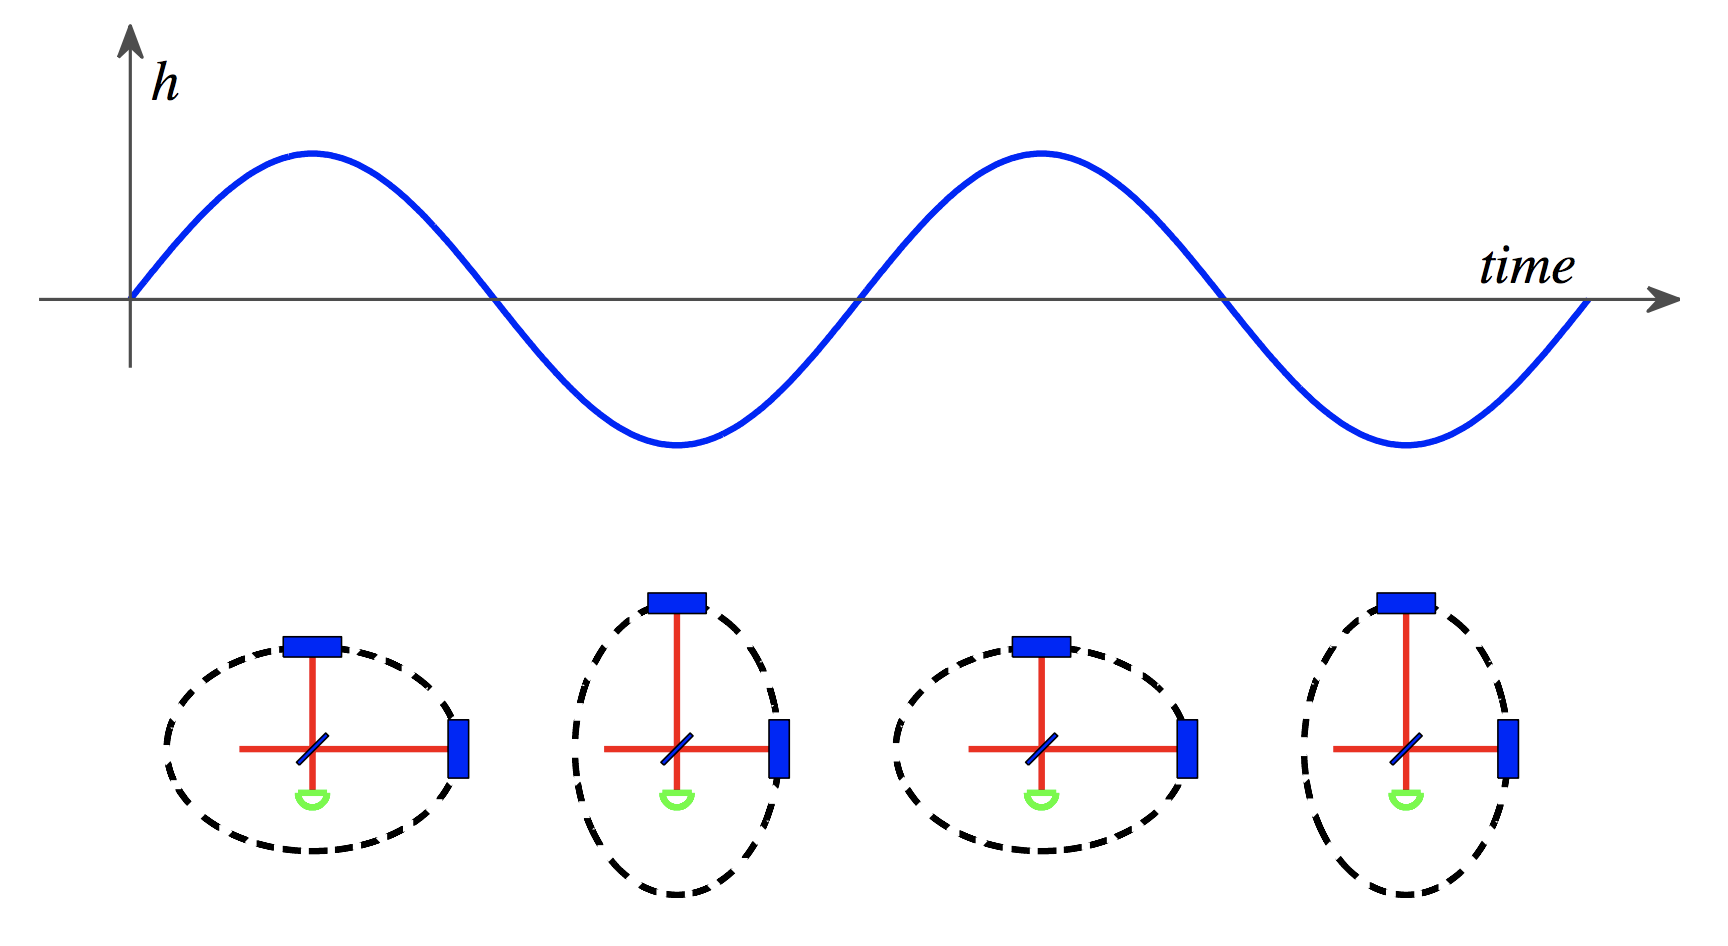
\includegraphics[width=10cm]{figures/StrainDiagram.png}
    \caption{\footnotesize{A GW traveling perpendicular to the plane of the diagram is characterized by a strain amplitude $h$. The wave distorts a ring of test particles into an ellipse, elongated in one direction in one half-cycle of the wave, and elongated in the orthogonal direction in the next half-cycle. This oscillating distortion can be measured with a Michelson interferometer oriented as shown. The length oscillations modulate the phase shifts accrued by the light in each arm, which are in turn observed as light intensity modulations at the photo-detector (green semi-circle). This depicts one of the linear polarization modes of the GW. Figure taken from Abbott et al. (2009).}}
    \label{fig:straindiagram}
\end{figure}

{\noindent}GWs differ from electromagnetic waves in that they propagate essentially unperturbed through space, as they interact only very weakly with matter. Furthermore, GWs are intrinsically non-linear, because the wave energy density itself generates additional curvature of space-time. This phenomenon is only significant, however, very close to strong sources of waves, where the wave amplitude is relatively large. More usually, GWs distinguish themselves from EM waves by the fact that they are very weak. One cannot hope to detect any waves of terrestrial origin, whether naturally occurring or man-made; instead one must look for very massive compact astrophysical objects, moving at relativistic velocities. For example, strong sources of GWs that may exist in our Galaxy or nearby galaxies are expected to produce wave strengths on Earth that do not exceed strain levels of one part in $10^{21}$. Finally, it is important to appreciate that GW detectors respond directly to GW amplitude rather than GW power; therefore the volume of space that is probed for potential sources increases as the cube of the strain sensitivity.


{\noindent}\textbf{Frequency bands, sources, and detection methods}: Four gravitational-wave frequency bands are being explored experimentally: the high-frequency band (HF; $\nu\sim1\,{\rm Hz}$ to $\nu\sim10^4\,{\rm Hz}$), the low-frequency band (LF; $1\,{\rm Hz}$ to $10^4\,{\rm Hz}$), the very-low frequency band (VLF; $10^7\,{\rm Hz}$ to $10^9\,{\rm Hz}$), and the extremely-low-frequency band (ELF; $10^{15}\,{\rm Hz}$ to $10^{18}\,{\rm Hz}$).

{\noindent}\textbf{HF band: $1\,{\rm Hz}$ to $10^4\,{\rm Hz}$}: A gravitational-wave source of mass $M$ cannot be much smaller than its gravitational radius, $2GM/c^2$, and cannot emit strongly at periods much smaller than the light-travel time $4GM/c^3$ around this gravitational radius. Correspondingly, the frequencies at which it emits are

\begin{align*}
    \nu \lesssim \frac{1}{4\pi GM/c^3} \sim 10^4 \frac{\rm M_\odot}{M} ~ [{\rm Hz}],
\end{align*}

{\noindent}where ${\rm M_\odot}$ is the mass of the Sun, and $G$ and $c$ are Newton's gravitation constant and the speed of light, respectively. To achieve a size of the same order as its gravitational radius and thereby emit near this maximum frequency, an object presumably must be heavier than the \textbf{Chandrasekhar limit}, about the mass of the sun, ${\rm M_\odot}$. Thus, the highest frequency expected for strong gravitational waves is $\nu_{\rm max}\sim10^4\,{\rm Hz}$. This defines the upper edge of the high-frequency gravitational-wave band. 

{\noindent}The HF band is the domain of the Earth-based gravitational-wave detectors of laser interferometers and resonant mass antennas. At frequencies below about $1\,{\rm Hz}$, Earth-based detectors face nearly insurmountable noise from:

\begin{enumerate}
    \item fluctuating Newtonian gravity gradients (due, e.g., to the gravitational pulls of inhomogeneities in the Earth's atmosphere which move overhead with the wind); and
    \item Earth vibrations (which are extremely difficult to filter out mechanically below $\sim1\,{\rm Hz}$).
\end{enumerate}

{\noindent}This defines the $1\,{\rm Hz}$ lower edge of the high-frequency band; to detect waves below this frequency, one must fly one's detectors in space.

{\noindent}A number of interesting gravitational-wave sources fall in the HF band: the stellar collapse to a neutron star or black hole in our Galaxy and distant galaxies, which sometimes triggers SNe; the rotation and vibration of neutron stars (pulsars) in our Galaxy; the coalescence of neutron-star and stellar-mass black-hole binaries ($M<1000\,{\rm M_\odot}$) in distant galaxies; and possibly such sources of stochastic background as vibrating loops of cosmic string, phase transitions in the early Universe, and the Big Bang in which the Universe was born.

{\noindent}\textbf{LF band: $10^{-4}\,{\rm Hz}$ to $1\,{\rm Hz}$}: The LF band is the domain of detectors flown in space (in Earth orbit or in interplanetary orbit). The most important of these are the Doppler tracking of spacecraft via microwave signals sent from Earth to the spacecraft and there transponded back to Earth (a technique that NASA has pursued since the early 1970s), and optical tracking of spacecraft by each other (laser interferometry in space, a technique now under development for possible flight in $\sim$2014 or sooner).

{\noindent}The $1\,{\rm Hz}$ upper edge of the LF band is defined by the gravity gradient and seismic cutoffs on Earth-based instruments; the  $10^{-4}\,{\rm Hz}$ lower edge is defined by expected severe difficulties at lower frequencies in isolating spacecraft from the buffeting forces of fluctuating solar radiation pressure, solar wind, and cosmic rays.

{\noindent}The LF band should be populated by waves from short-period binary stars in our own Galaxy (MS binaries, cataclysmic variables, white-dwarf binaries, neutron-star binaries, etc.); from white dwarfs, neutron stars, and small black holes spiraling into massive black holes ($M\sim3\times10^5\,{\rm M_\odot}$ to $3\times10^7\,{\rm M_\odot}$) in distant galaxies; and from the inspiral and coalescence of super-massive black-hole binaries ($M\sim100\,{\rm M_\odot}$ to $10^8\,{\rm M_\odot}$). The upper limit, $10^8\,{\rm M_\odot}$, on the masses of black holes that can emit in the LF band is set by 

\begin{align*}
    \nu \lesssim \frac{1}{4\pi GM/c^3} \sim 10^4 \frac{\rm M_\odot}{M} ~ [{\rm Hz}],
\end{align*}

{\noindent}with $\nu>10^4\,{\rm Hz}$. There should also be a LF stochastic background from such early-Universe processes as vibrating cosmic strings, phase transitions, and the Big Bang itself.

{\noindent}\textbf{VLF band: $10^{-9}\,{\rm Hz}$ to $10^{-7}\,{\rm Hz}$}: Joseph Taylor and others have achieved a remarkable gravity-wave sensitivity in the VLF band by the timing of millisecond pulsars. When a gravitational wave passes over the Earth, it perturbs our rate of flow of time and hence the ticking rates of our clocks relative to clocks outside the wave. Such perturbations will show up as apparent fluctuations in the times of arrival of the pulsar's pulses. If no fluctuations are seen at some level, we can be rather sure that neither Earth nor the pulsar is being bathed by gravitational waves of the corresponding strength. If fluctuations with the same time evolution are seen simultaneously in the timing of several different pulsars, then the cause could well be gravitational waves bathing the Earth.

{\noindent}By averaging the pulses' times of arrival over long periods of time (months to tens of years), a very high timing precision can be achieved, and correspondingly, tight limits can be placed on the waves bathing the Earth or the pulsar. The upper edge of the VLF band, $\sim10^7\,{\rm Hz}$, is set by the averaging time of a few months needed to build up high accuracy; the lower edge, $\sim10^9\,{\rm Hz}$, is set by the time of $\sim20$ years, since very steady millisecond pulsars were first discovered.

{\noindent}Strong gravitational-wave sources are generally compact, not much larger than their own gravitational radii. The only compact bodies that can radiate in the VLF band or below (i.e., at $\nu<10^7\,{\rm Hz}$) are those with $M>10^{11}\,{\rm M_\odot}$. Conventional astronomical wisdom suggests that compact bodies this massive do not exist, and that therefore, the only strong waves in the VLF band and below are a stochastic background produced by the same early-Universe processes as might radiate at low and high frequencies: cosmic strings, phase transitions, and the Big Bang.

{\noindent}Of course, conventional wisdom could be wrong. Nevertheless, it is conventional to quote measurement accuracies in the VLF band and below in the language of a stochastic background: the fraction $\Omega_g(\nu)$ of the energy required to close the Universe that lies in a bandwidth $\Delta\nu=\nu$ centered on frequency $\nu$. The current $95\%$ confidence limit on  $\Omega_g(\nu)$ from pulsar timing in the VLF band is  $\Omega_g(4\times10^9\,{\rm Hz})<6\times10^{-8}H^{-2}$, where $H$ is the Hubble constant in units of $100\,{\rm km\,s^{-1}\,Mpc^{-1}}$. This is a sufficiently tight limit that is beginning to cast doubt on the (not terribly popular) suggestion that the Universe contains enough vibrating loops of cosmic string for their gravitational pulls to have seeded galaxy formation.

{\noindent}\textbf{ELF band: $10^{-18}\,{\rm Hz}$ to $10^{-15}\,{\rm Hz}$}: Gravitational waves in the ELF band should produce anisotropies in the CMB. The tightest limit from microwave observations comes from the lower edge of the ELF band $\nu\sim10^{-18}\,{\rm Hz}$, where the gravitational wavelength is about $\pi$ times the Hubble distance, and the waves, by squeezing all of the space inside our cosmological horizon in one direction and stretching it all in another, should produce a quadrupolar anisotropy in the CMB. The quadrupolar anisotropy measured by the COBE satellite, if due primarily to gravitational waves (which it could be), corresponds to an energy density $\Omega_g(10^{-18}\,{\rm Hz})\sim10^{-9}$.

\begin{figure}[h]
    \centering
    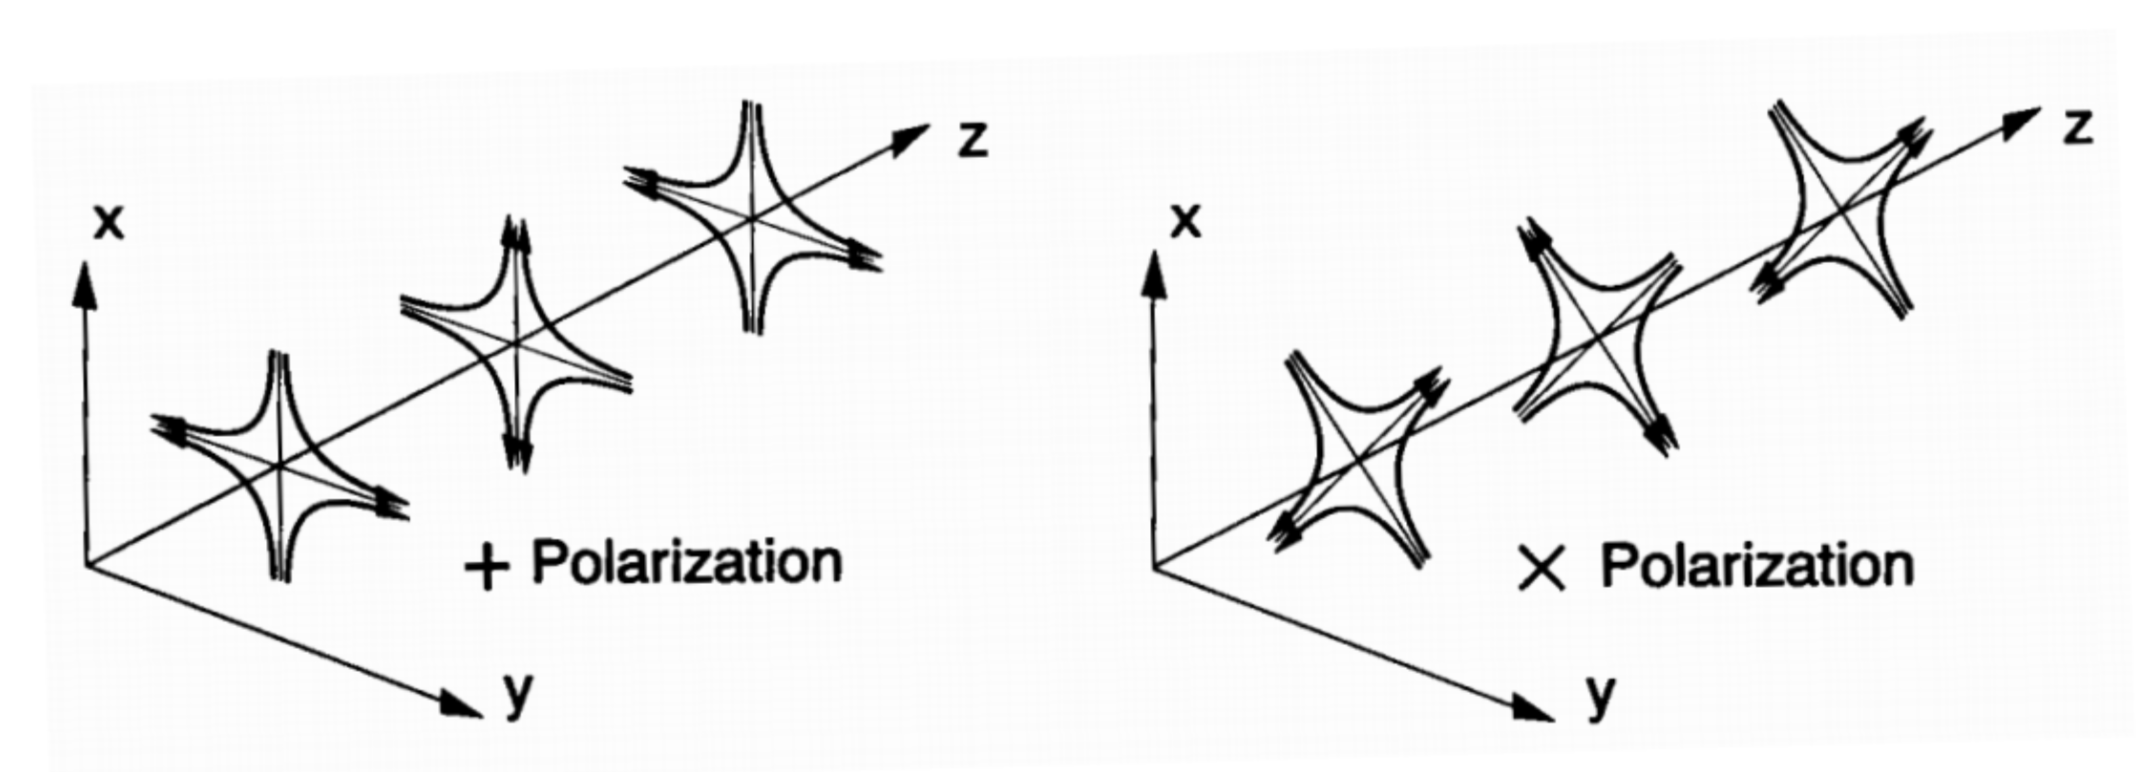
\includegraphics[width=15cm]{figures/ForceLines.png}
    \caption{\footnotesize{The lines of force associated with the two polarizations of a gravitational wave. Figure taken from Thorne (1994).}}
    \label{fig:forcelines}
\end{figure}

{\noindent}\textbf{Wave polarizations, waveforms, and how an interferometer works}: According to general relativity theory (which we shall assume to be correct), a gravitational wave has two linear polarizations, conventionally called $+$ (\textbf{plus}) and $\times$ (\textbf{cross}). Associated with each polarization, there is a gravitational wave field, $hP_+$ or $h_\times$, which oscillates in time and propagates with the speed of light. Each wave field produces tidal forces (stretching and squeezing forces) on any object or detector through which it passes. If the object is small compared to the waves' wavelength (as is the case for ground-based interferometers and resonant mass antennas), then relative to the object's center, the forces have the quadrupolar patterns shown in Figure \ref{fig:forcelines}. The names ``plus'' and ``cross'' are derived from the orientations of the axes that characterize the force patterns.

{\noindent}A laser interferometer gravitational wave detector (\textbf{interferometer} for short) consists of four masses that hang from vibration-isolated supports as shown in Figure \ref{fig:interferometer}, and the indicated optical system for monitoring the separations between the masses. Two masses are near each other, at the corner of an ``L,'' and one mass is at the end of each of the L's long arms. The arm lengths are nearly equal, $L_1\simeq L_2=L$. When a gravitational wave, with high frequencies compared to the masses' $\sim1\,\,{\rm Hz}$ pendulum frequency, passes through the detector, it pushes the masses back and forth relative to each other as though they were free from their suspension wires, thereby changing the arm-length difference, $\Delta L\equiv L_1-L_2$. That change is monitored by laser interferometry in such a way that the variations in the output of the photodiode (the interferometer's output) are directly proportional to $\Delta L(t)$.

{\noindent}If the waves are coming from overhead or underfoot, and the axes of the $+$ polarization coincide with the arms' directions, then it is the wave's $+$ polarization that drives the masses, and $\Delta L(t)/L=h_+(t)$. More generally, the interferometer's output is a linear combination of the two wave fields:

\begin{align*}
    \frac{\Delta L}{L} = F_+h_+(t) + F_\times h_\times(t) \equiv h(t) ~ [{\rm dimensionless}].
\end{align*}

{\noindent}The coefficients $F_+$ and $F_\times$ are of order unity and depend in a quadrupolar manner on the direction to the source and the orientation of the detector. The combination $h(t)$ of the two $h$'s is called the \textbf{gravitational-wave strain} that acts on the detector; and the time evolutions of $h_+(t)$, $h_\times(t)$, and $h(t)$ are sometimes called \textbf{waveforms}.

{\noindent}Interferometer test masses at present are made of transparent fused silica, though other materials might be used in the future. The masses' inner faces (shown white in Figure \ref{fig:interferometer}) are covered with high-reflectivity dielectric coatings to form the indicated ``mirrors,'' while the masses' outer faces are covered with anti-reflection coatings. The two mirrors facing each other on each arm form a \textbf{Fabry-Perot} cavity. A \textbf{beam splitter} splits a carefully prepared laser beam in two and directs the resulting beams down the two arms. Each beam penetrates through the anti-reflection coating of its arm's corner mass, through the mass, and through the dielectric coating (the mirror); and thereby -- with the length of the arm's Fabry-Perot cavity adjusted to be nearly an integral number of half wavelengths of light -- the beam gets trapped in the cavity. The cavity's end mirror has much higher reflectivity than its corner mirror, so the trapped light leaks back out
through the corner mirror and then hits the beam splitter where it recombines with light from the other arm. Most of the recombined light goes back toward the laser (where it can be returned to the interferometer by a \textbf{light-recycling mirror}
labeled $R$), but a tiny portion goes toward the photodiode.

\begin{figure}[t]
    \centering
    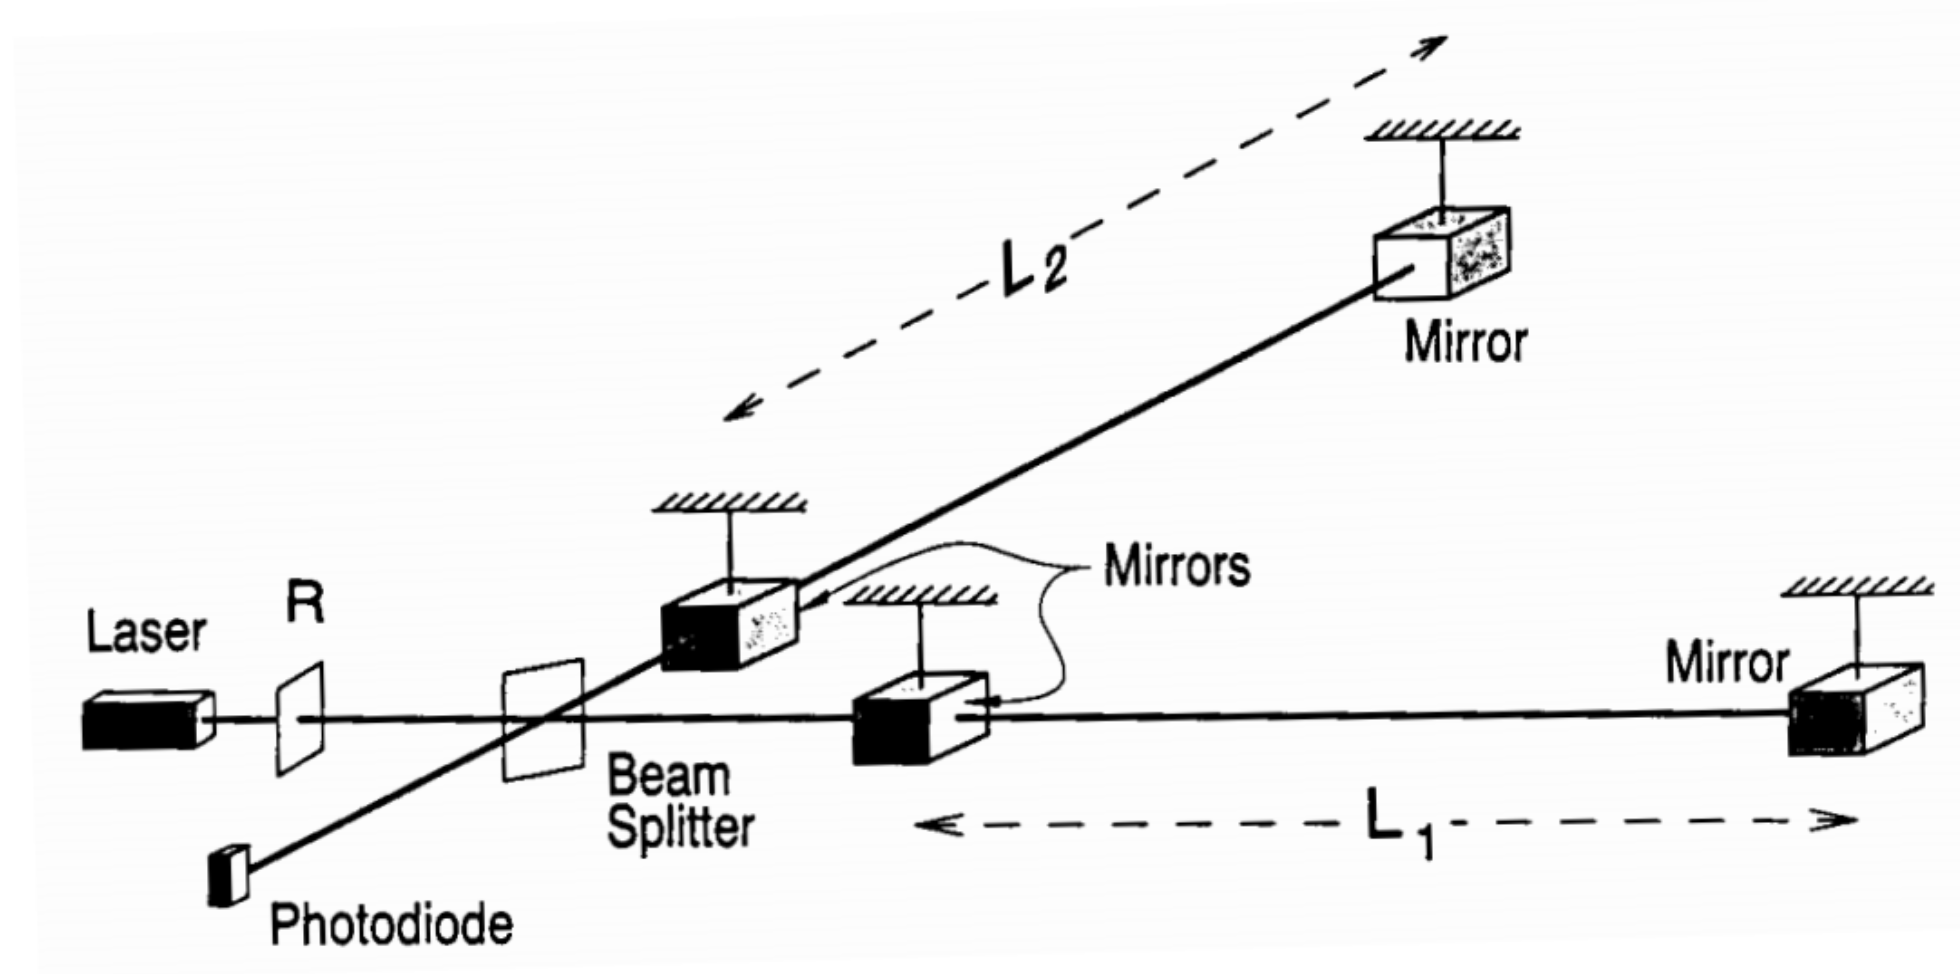
\includegraphics[width=12cm]{figures/interferometer.png}
    \caption{\footnotesize{Schematic diagram of a laser interferometer gravitational wave detector. Figure taken from Thorne (1994).}}
    \label{fig:interferometer}
\end{figure}

{\noindent}When a gravitational wave hits the detector and moves the masses, thereby changing the lengths $L_1$ and $L_2$ of the two cavities, it shifts each cavity's resonant frequency slightly relative to the laser frequency, and thereby changes the phase of the light in the cavity and the phase of the light that exits from the cavity toward the beam splitter. Correspondingly, the relative phase of the two beams returning to the splitter is altered by an amount $\Delta\Phi\propto\Delta L$, and this relative phase shift causes a change in the intensity of the recombined light at the photodiode, $I_{\rm pd}\propto\Delta L\propto h(t)$. Thus, the change of photodiode output current is directly proportional to the gravitational-wave strain $h(t)$. This method of monitoring $h(t)$, which was invented by Ronald Drever as a modification of Rainer Weiss's seminal concept for such an interferometer, is capable of very high sensitivity.

{\noindent}\textbf{Wave strengths and interferometer arm lengths}: The strengths of the waves from a gravitational-wave source can be estimated using the ``Newtonian quadrupole'' approximation to the Einstein field equations. This approximation says that $h\simeq(G/c^4)\ddot{Q}/r$, where $\ddot{Q}$ is the second time derivative of the source's quadrupole moment, $r$ is the distance of the source from Earth, and $G$ and $c$ are Newton's gravitation constant and the speed of light, respectively. The strongest sources will be highly non-spherical, and thus, will have $Q\simeq ML^2$ where $M$ is their mass and $L$ their size, and correspondingly, will have $\ddot{Q}\simeq2Mv^2\simeq4E_{\rm kin}^{\rm ns}$ where $v$ is their internal velocity and $E_{\rm kin}^{\rm ns}$ is the non-spherical part of their internal
kinetic energy. This provides us with the estimate

\begin{align*}
    h \sim \frac{1}{c^2} \frac{4G(E_{\rm kin}^{\rm ns}/c^2)}{r}  ~ [{\rm dimensionless}],
\end{align*}

{\noindent}that is, $h$ is about four times the gravitational potential produced at Earth by the mass-equivalent of the source's non-spherical, internal kinetic energy, made dimensionless by dividing by $c^2$. Thus, in order to radiate strongly, the source must have a very large, non-spherical internal kinetic energy.

{\noindent}The best known way to achieve a huge internal kinetic energy is via gravity; and by energy conservation (or the virial theorem), any gravitationally-induced kinetic energy must be of the order of the source's gravitational potential energy. A huge potential energy, in turn, requires that the source be very compact, not much larger than its own gravitational radius. Thus, the strongest gravity-wave sources must be highly compact, dynamical concentrations of large amounts of mass (e.g., colliding and coalescing black holes and neutron stars).

{\noindent}Such sources cannot remain highly dynamical for long; their motions will be stopped by energy loss to gravitational waves and/or the formation of an all-encompassing black hole. Thus, the strongest sources should be transient. More-over, they should be very rare; so rare that to see a reasonable event rate will require reaching out through a substantial fraction of the Universe. Thus, just as the strongest radio waves arriving at Earth tend to be extragalactic, so also the strongest gravitational waves are likely to be extragalactic.

{\noindent}For highly compact, dynamical objects that radiate in the high-frequency band (e.g., colliding and coalescing neutron stars and stellar-mass black holes), the internal, non-spherical kinetic energy $E_{\rm kin}^{\rm ns}/c^2$ is of the order of the mass of the Sun; and, correspondingly, $h\sim10^{-22}$ for such sources at the Hubble distance ($3000\,{\rm Mpc}$, i.e., $10^{10}$ light years); $h\sim10^{-21}$ at $200\,{\rm Mpc}$ (a best-guess distance for several neutron-star coalescences per year), $h\sim10^{- 20}$ at the Virgo cluster of galaxies ($15\,{\rm Mpc}$); and $h\sim10^{-17}$ in the outer reaches of our own Milky Way galaxy ($20\,{\rm kpc}$). These numbers set the scale of sensitivities that ground-based interferometers seek to achieve: $h\sim10^{-21}$ to $10^{-22}$.

{\noindent}When one examines the technology of laser interferometry, one sees good prospects to achieve measurement accuracies $\Delta L\sim10^{-16}\,{\rm cm}$ ($1/1000$ the diameter of the nucleus of an atom). With such an accuracy, an interferometer must have an arm length $L=\Delta L/h\sim1$ to $10\,{\rm km}$ in order to achieve the desired wave sensitivities of $10^{-21}$ to $10^{-22}$.

{\noindent}\textbf{LIGO and the worldwide detector network}: As illustrated in Figure \ref{fig:straindiagram}, the oscillating quadrupolar strain pattern of a GW is well matched by a Michelson interferometer, which makes a very sensitive comparison of the lengths of its two orthogonal arms. LIGO utilizes three specialized Michelson interferometers, located at two sites (see Figure \ref{fig:ligo}): an observatory on the Hanford site in Washington houses two interferometers, the 4 km-long H1 and 2 km-long H2 detectors; and an observatory in Livingston Parish, Louisiana, houses the 4 km-long L1 detector. Other than the shorter length of H2, the three interferometers are essentially identical. Multiple detectors at separated sites are crucial for rejecting instrumental and environmental artifacts in the data, by requiring coincident detections in the analysis. Also, because the antenna pattern of an interferometer is quite wide, source localization requires triangulation using three separated detectors.

{\noindent}The initial LIGO detectors were designed to be sensitive to GWs in the frequency band $40-7000\,{\rm Hz}$, and capable of detecting a GW strain amplitude as small as $10^{-21}$. With funding from the National Science Foundation, the LIGO sites and detectors were designed by scientists and engineers from the California Institute of Technology and the Massachusetts Institute of Technology, constructed in the late 1990s, and commissioned over the first 5 years of this decade. From November 2005 to September 2007, they operated at their design sensitivity in a continuous data-taking mode. The data from this science run, known as S5, were analyzed for a variety of GW signals by a group of researchers known as the LIGO Scientific Collaboration. At the most sensitive frequencies, the instrument rms strain noise has reached an unprecedented level of $3\times10^{-22}$ in a $100\,{\rm Hz}$ band.

\begin{figure}[t]
    \centering
    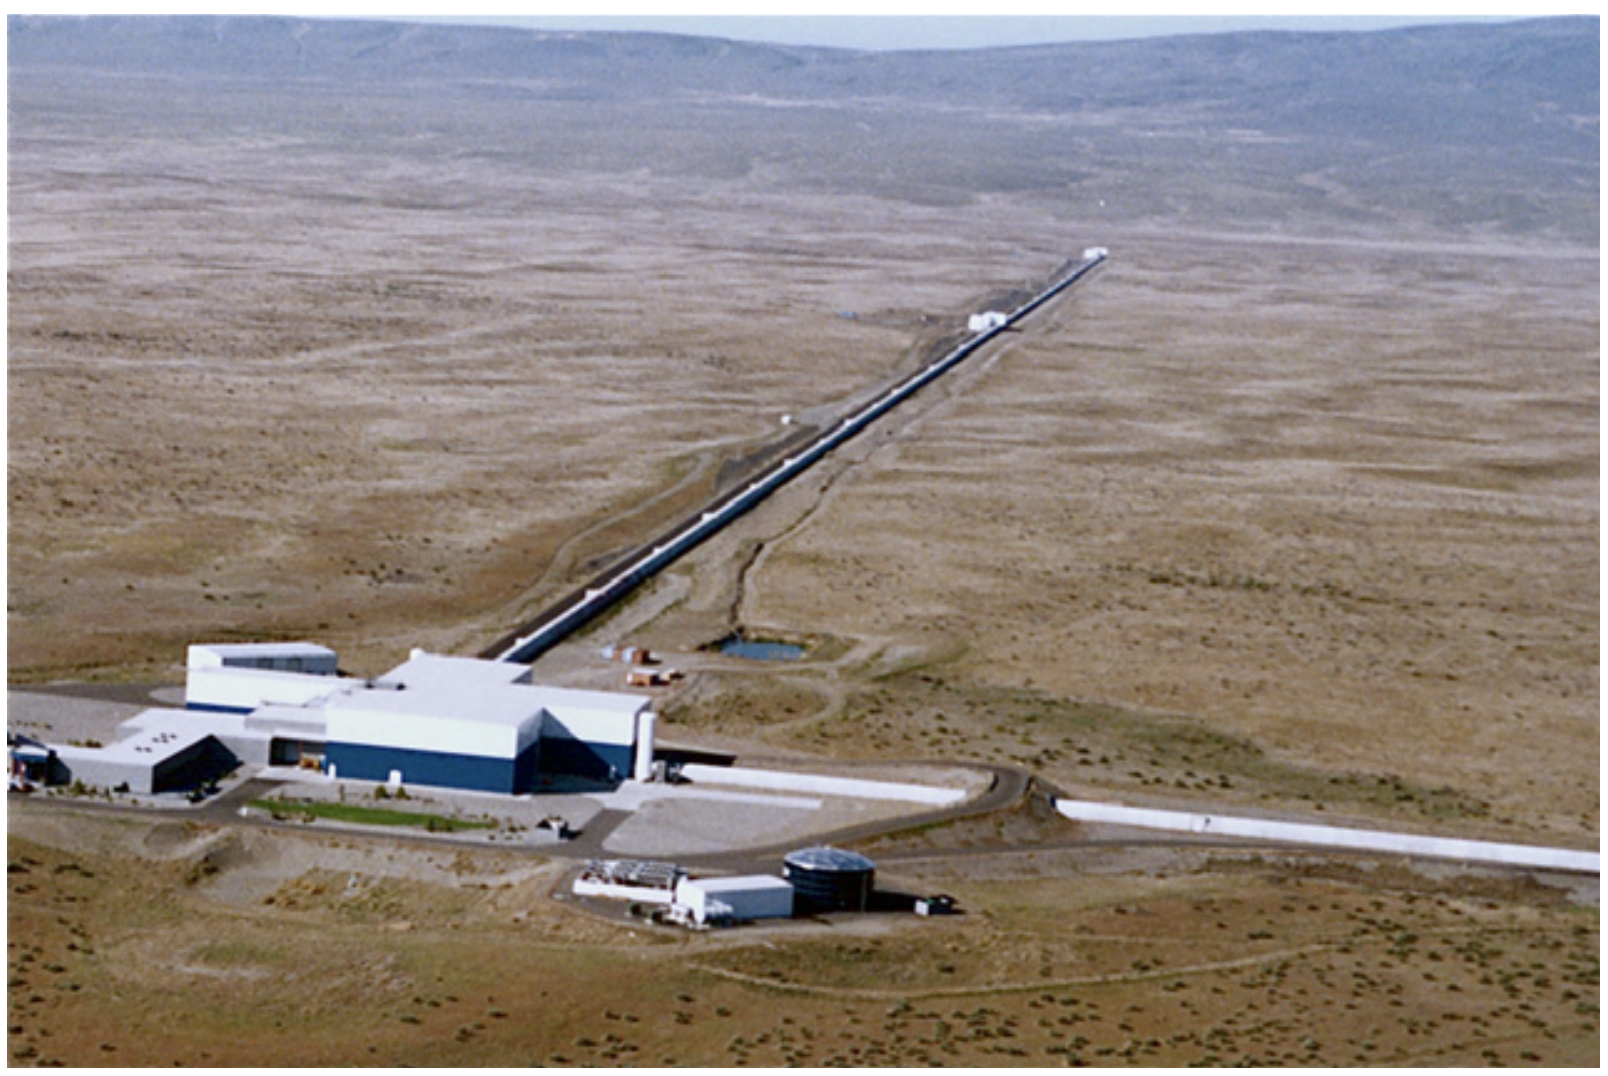
\includegraphics[width=7.5cm]{figures/LIGO_Washington.png}
    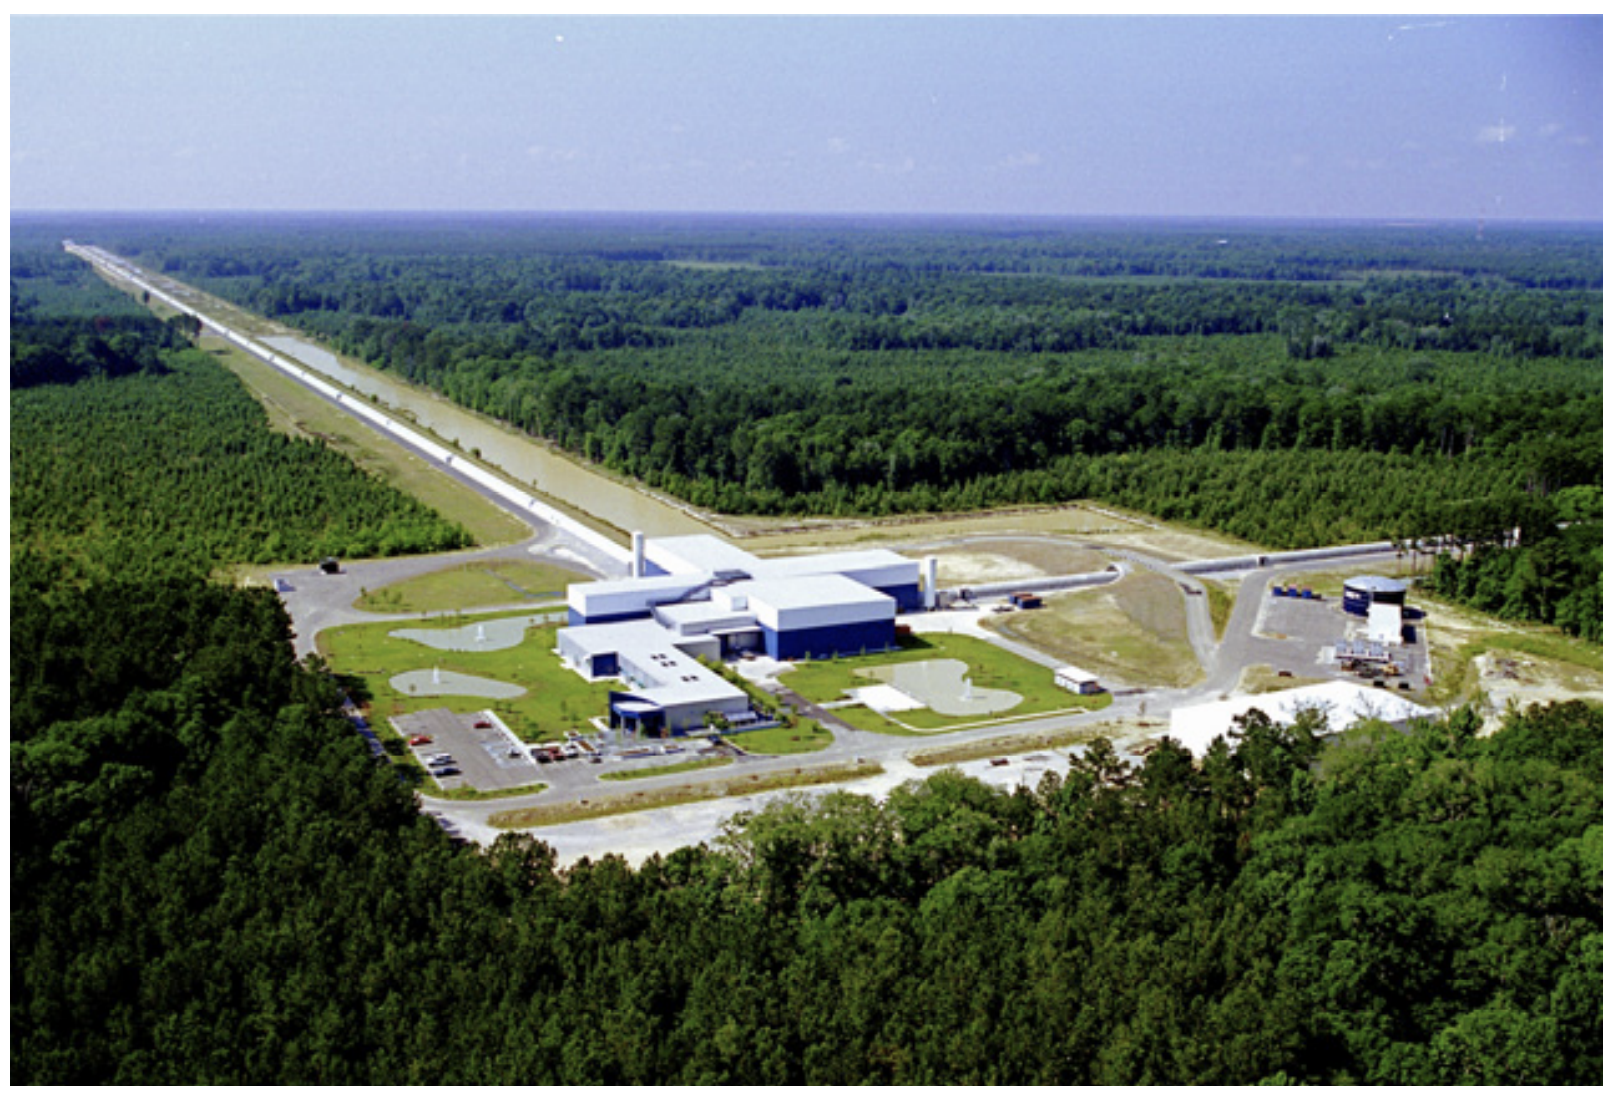
\includegraphics[width=7.5cm]{figures/LIGO_Louisiana.png}
    \caption{\footnotesize{Aerial photograph of the LIGO observatories at Hanford, Washington \textbf{(left)} and Livingston, Louisiana \textbf{(right)}. The lasers and optics are contained in the large corner buildings. From each corner building, evacuated beam tubes extend at right angles for 4 km in each direction (the full length of only one of the arms is seen in each photo); the tubes are covered by the arched, concrete enclosures seen here. Figure taken from Abbott (2009).}}
    \label{fig:ligo}
\end{figure}

{\noindent}Although in principle LIGO can detect and study GWs by itself, the potential to do astrophysics can be quantitatively and qualitatively enhanced by operation in a more extensive network. For example, the direction of travel of the GWs and the complete polarization information carried by the waves can only be extracted by a network of detectors. Such a global network of GW observatories has been emerging over the past decade. In this period, the Japanese TAMA project built a $300\,{\rm m}$ interferometer outside Tokyo, Japan; the German-British GEO project built a $600\,{\rm m}$ interferometer near Hanover, Germany; and the European Gravitational Observatory built the 3 km-long interferometer Virgo near Pisa, Italy. In addition, plans are underway to develop a large scale GW
detector in Japan sometime during the next decade.

{\noindent}Early in its operation LIGO joined with the GEO project; for strong sources the shorter, less sensitive GEO 600 detector provides added confidence and directional and polarization information. In May 2007 the Virgo detector began joint observations with LIGO, with a strain sensitivity close to that of LIGO's $4\,{rm km}$ interferometers at frequencies above $\sim1\,{\rm\,kHz}$. The LIGO Scientific Collaboration and the Virgo Collaboration negotiated an agreement that all data collected from that date would be analyzed and published jointly.

{\noindent}\textbf{LIGO instrument performance and noise}: The challenge is to make the instrument sufficiently sensitive: at the targeted strain sensitivity of $10^{-21}$, the resulting arm length change is only $\sim10^{-18}\,{\rm m}$, a thousand times smaller than the diameter of a proton. Meeting this challenge involves the use of special interferometry techniques, state-of-the-art optics, highly stable lasers and multiple layers of vibration isolation. And of course a key feature of the detectors is simply their scale: the arms are made as long as practically possible to increase the signal due to a GW strain.

{\noindent}The response of the interferometer output is a function of GW frequency and is derived in length in other papers. In the long-wavelength approximation, where the wavelength of the GW is much longer than the size of the detector, the response $R$ of a Michelson-Fabry-Perot interferometer is approximated by a single-pole transfer function:

\begin{align*}
    R(\nu) \propto \frac{1}{1+i\nu/\nu_p},
\end{align*}

{\noindent}where the pole frequency $\nu_p$ is related to the arm cavity storage time by $\nu_p=1/4\pi\tau_s$. Above the pole frequency ($\nu_p=85\,{\rm Hz}$ for the LIGO $4 km$ interferometers), the amplitude response drops off as $1/\nu$. The measurement noise above the pole frequency has a white (flat) spectrum, and so the strain sensitivity decreases proportionally to frequency in this region. The single-pole approximation is quite accurate, differing from the exact response by less than a percent up to $\sim1\,{\rm kHz}$.

{\noindent}In the long-wavelength approximation, the interferometer directional response is maximal for GWs propagating orthogonally to the plane of the interferometer arms and linearly polarized along the arms. Other angles of incidence or polarizations give a reduced response, as depicted by the antenna patterns shown in Figure \ref{fig:ligopsf}. A single detector has blind spots on the sky for linearly polarized GWs.

\begin{figure}[t]
    \centering
    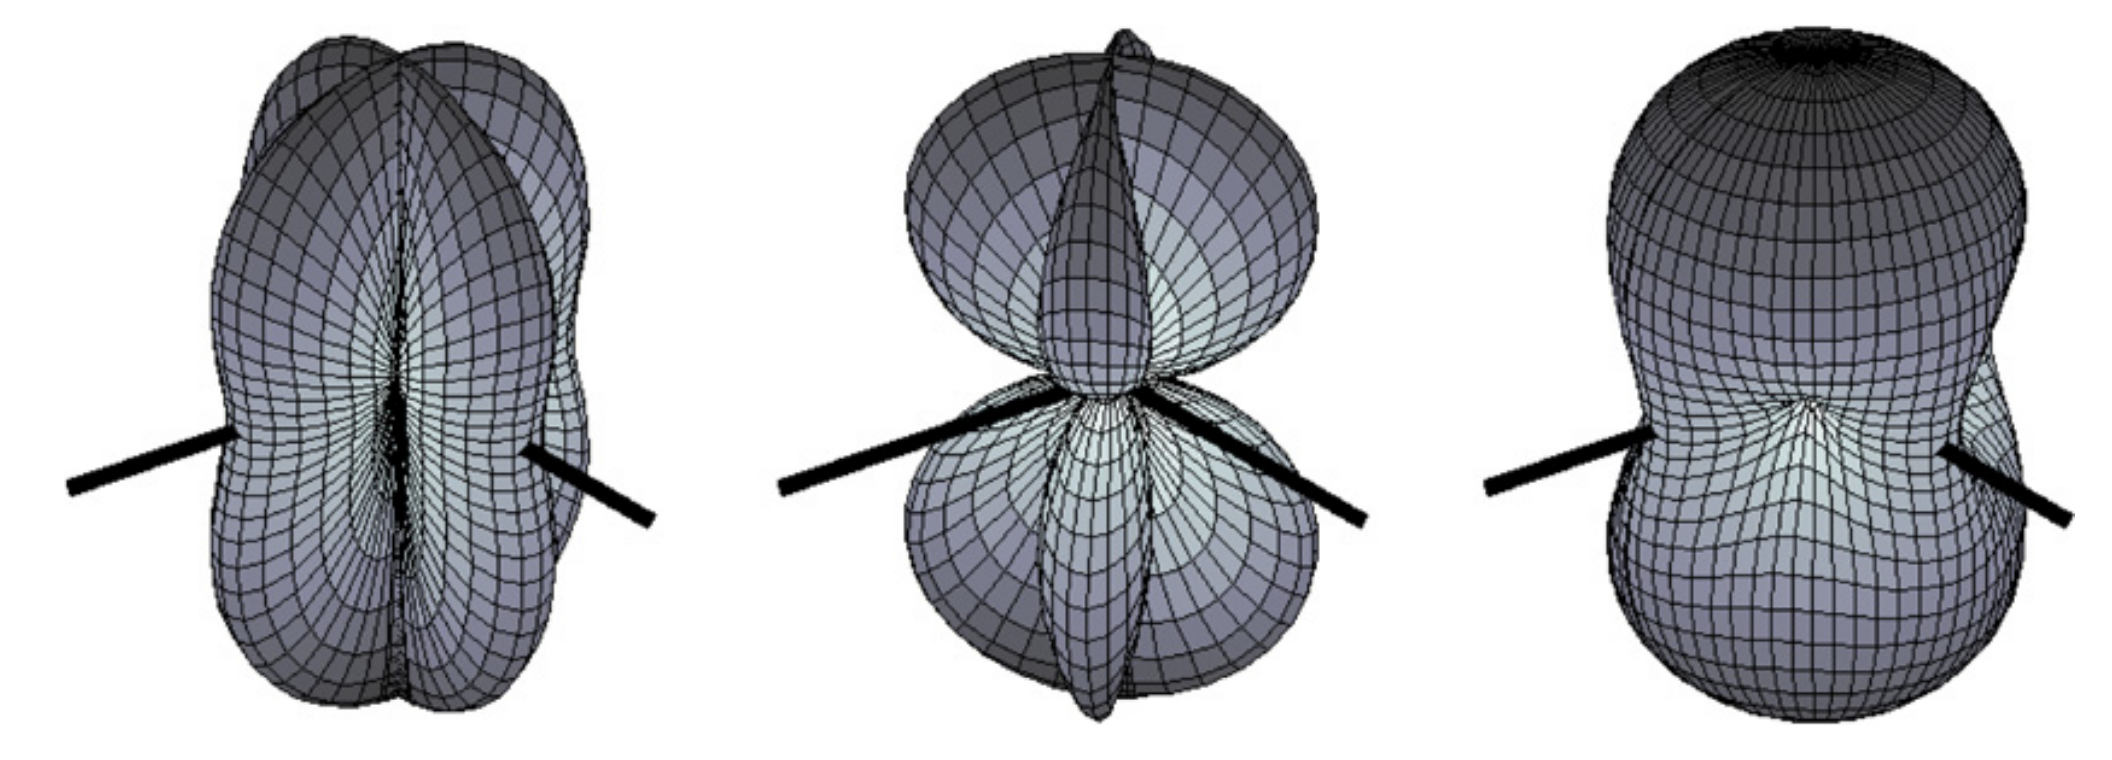
\includegraphics[width=12cm]{figures/LIGO_PSF.png}
    \caption{\footnotesize{Antenna response pattern for a LIGO GW detector, in the long-wavelength approximation. The interferometer beamsplitter is located at the center of each pattern, and the thick black lines indicate the orientation of the interferometer arms. The distance from a point of the plot surface to the center of the pattern is a measure of the GW sensitivity in this direction. The pattern on the left is for $+$ polarization, the middle pattern is for $\times$ polarization, and the right-most one is for unpolarized waves. Figure taken from Abbott (2009).}}
    \label{fig:ligopsf}
\end{figure}

{\noindent}To complete the LIGO detector, the interferometers were supplemented with a set of sensors to monitor the local environment. Seismometers and accelerometers measure vibrations of the ground and various interferometer components; microphones monitor acoustic noise at critical locations; magnetometers monitor fields that could couple to the test masses or electronics; radio receivers monitor RF power around the modulation frequencies. These sensors are used to detect environmental disturbances that can couple to the GW channel.

{\noindent}Since the interferometers detect GW strain amplitude, their performance is typically characterized by an amplitude spectral density of detector noise (the square root of the power spectrum), expressed in equivalent GW strain. Typical high-sensitivity strain noise spectra are shown in Figure \ref{fig:strainnoise}. Over the course of S5 the strain sensitivity of each interferometer was improved, by up to $40\%$ compared with the beginning of the run through a series of incremental improvements to the instruments.

\begin{figure}[h]
    \floatbox[{\capbeside\thisfloatsetup{capbesideposition={right,top},capbesidewidth=4cm}}]{figure}[\FBwidth]
    {\caption{\footnotesize{\\Strain sensitivities, expressed as amplitude spectral densities of detector noise converted to equivalent GW strain. The vertical axis denotes the rms strain noise in $1\,{\rm Hz}$ of bandwidth. Shown are typical high sensitivity spectra for each of the three interferometers (red: H1; blue: H2; green: L1), along with the design goal for the $4\,{\rm km}$ detectors (dashed gray). Figure taken from Abbott et al (2009).}}
    \label{fig:strainnoise}}
    {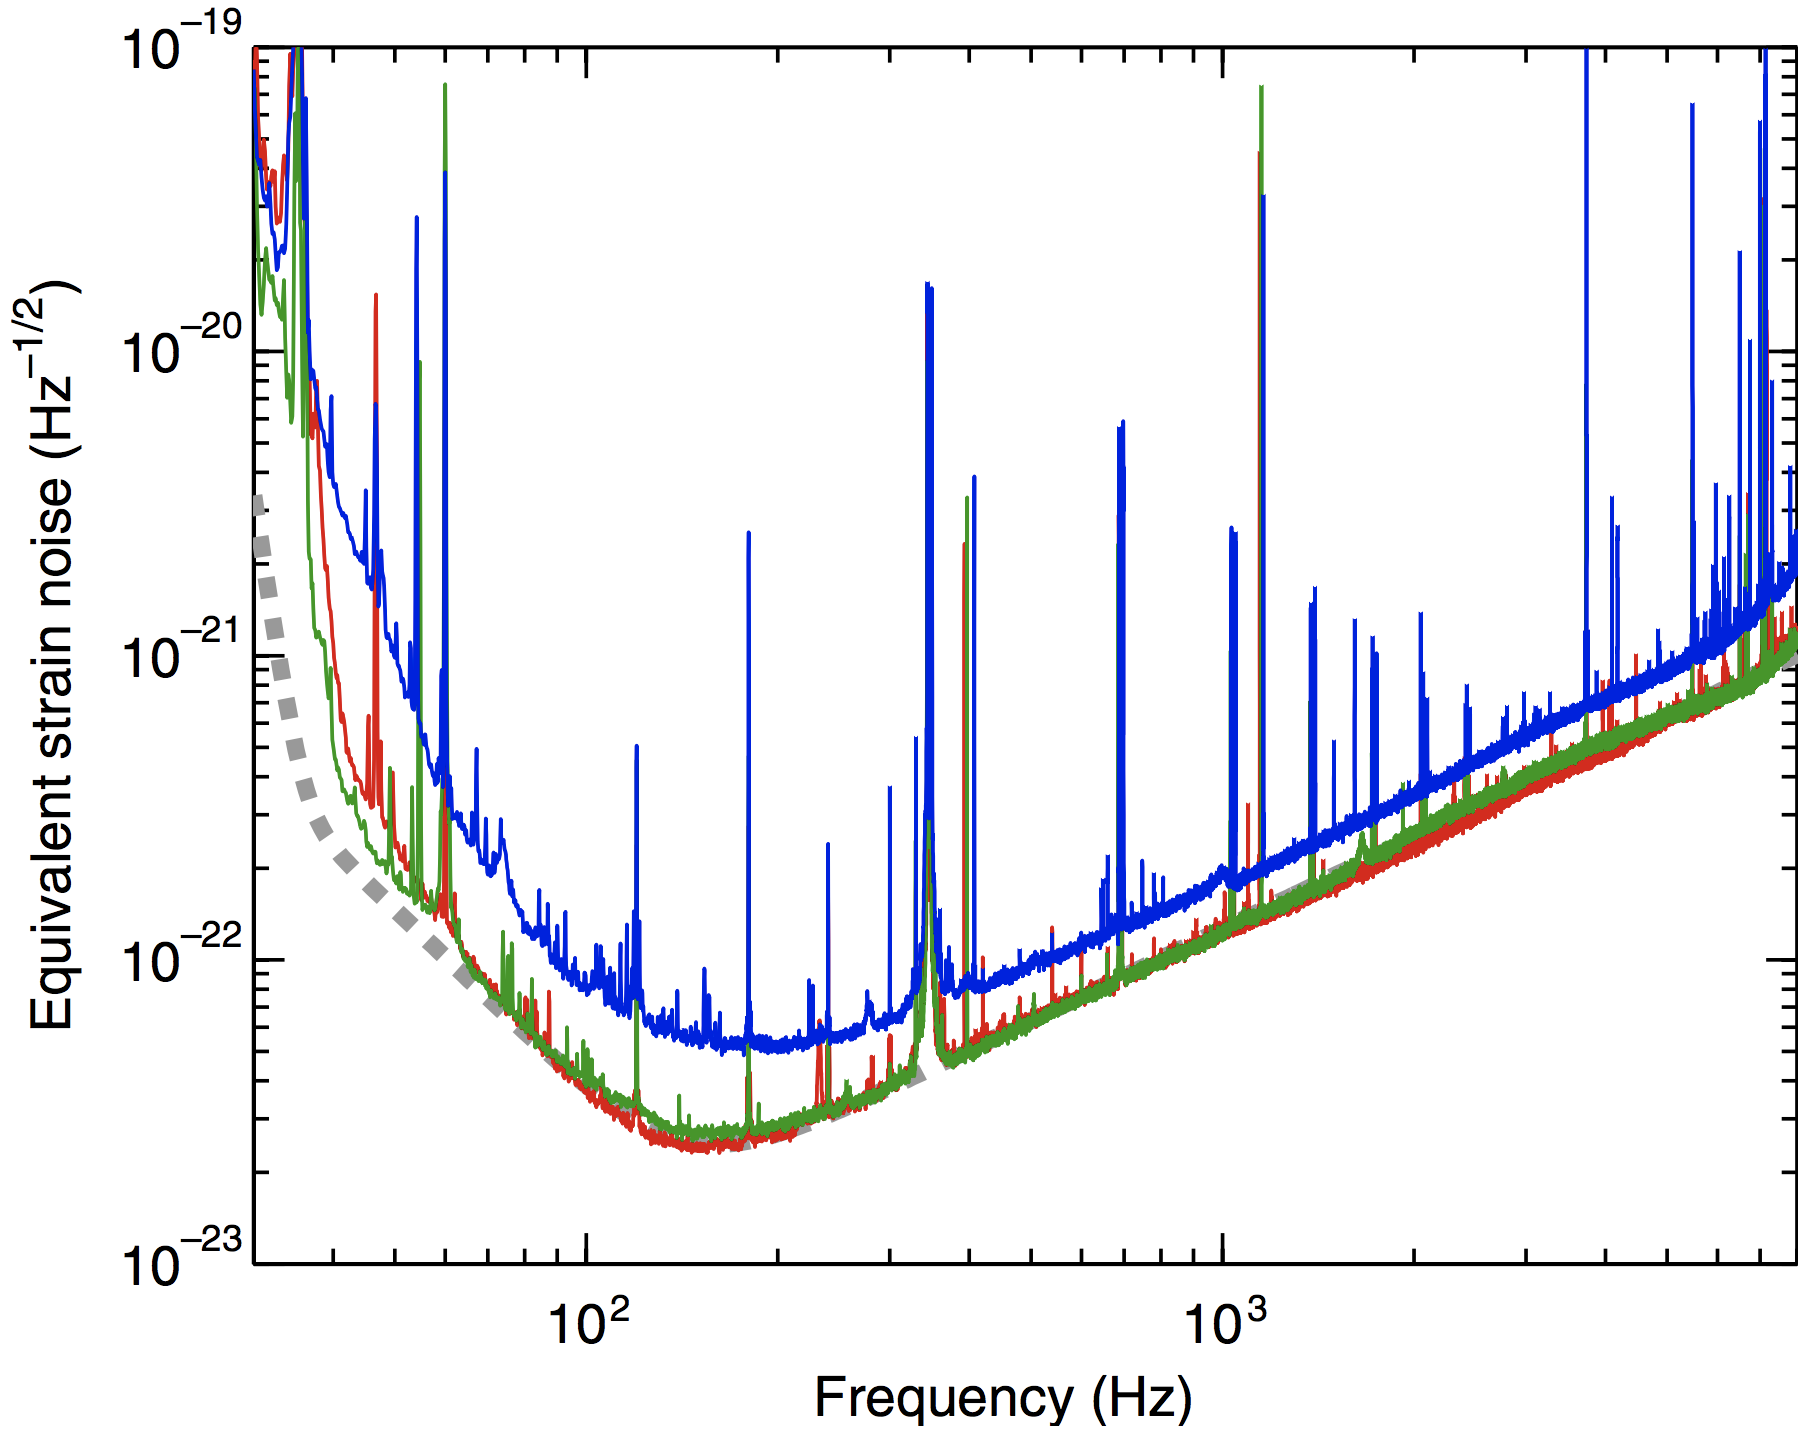
\includegraphics[width=10cm]{figures/StrainNoise.png}}
\end{figure}

{\noindent}The primary noise sources contributing to the H1 strain noise spectrum are shown in Figure \ref{fig:strainnoise}. Understanding and controlling these instrumental noise components has been the major technical challenge in the development of the detectors. The noise terms can be broadly divided into two classes: displacement noise and sensing noise. \textbf{Displacement noises} cause motions of the test masses or their mirrored surfaces. \textbf{Sensing noises}, on the other hand, are phenomena that limit the ability to measure those motions; they are present even in the absence of test mass motion. The strain noises shown in Figure \ref{fig:strainnoise} consist of spectral lines superimposed on a continuous broadband noise spectrum. The majority of the lines are due to power lines ($60$, $120$, $180\,{\rm Hz}$, etc.), ``violin mode'' mechanical resonances ($350$, $700\,{\rm Hz}$, etc) and calibration lines ($55$, $400$ and $1100\,{\rm Hz}$). These narrow noise lines are easily excluded from analysis; the broadband noise dominates the instrument sensitivity.

{\noindent}The left panel of Figure \ref{fig:ligonoise} shows the displacement noise. At the lowest frequencies the largest such noise is \textbf{seismic noise} -- motions of the Earth's surface driven by wind, ocean waves, human activity and low-level earthquakes; filtered by the isolation stacks and pendulums. The seismic contribution is estimated using accelerometers to measure the vibration at the isolation stack support points, and propagating this motion to the test masses using modeled transfer functions of the stack and pendulum. The seismic wall frequency, below which seismic noise dominates, is approximately $45\,{\rm Hz}$, a bit higher than the goal of $40\,{\rm Hz}$, as the actual environmental vibrations around these frequencies are $\sim10$ times higher than what was estimated in the design.

{\noindent}\textbf{Mechanical thermal noise} is a more fundamental effect, arising from finite losses present in all mechanical systems, and is governed by the \textbf{fluctuation-dissipation theorem}. It causes arm length noise through thermal excitation of the test mass pendulums (\textbf{suspension thermal noise}), and thermal acoustic waves that perturb the test mass mirror surface (\textbf{test mass thermal noise}). Most of the thermal energy is concentrated at the resonant frequencies, which are designed (as much as possible) to be outside the detection band. Away from the resonances, the level of thermal motion is proportional to the mechanical dissipation associated with the motion. Designing the mirror and its pendulum to have very low mechanical dissipation reduces the detection-band thermal noise. It is difficult, however, to accurately and unambiguously establish the level of broadband thermal noise in situ; instead, the thermal noise curves in Figure \ref{fig:ligonoise} are calculated from models of the suspension and test masses, with mechanical loss parameters taken from independent characterizations of the materials.

{\noindent}The right panel of Figure \ref{fig:ligonoise} shows the sensing noise. By design, the dominant noise source above $100\,{\rm Hz}$ is \textbf{shot noise}, as determined by the Poisson statistics of photon detection. The ideal shot-noise limited strain noise density, $\bar{h}(f)$, for this type of interferometer is

\begin{align*}
    \bar{h}(f) = \sqrt{\frac{\pi\hbar\lambda}{\eta P_{\rm BS}c}} \frac{\sqrt{1+(4\pi \nu\tau_s)^2}}{4\pi\tau_s} ~ [{\rm dimensionless}],
\end{align*}

{\noindent}where $\lambda$ is the laser wavelength, $\hbar$ is the reduced Planck constant, $c$ is the speed of light, $\tau_s$ is the arm cavity storage time, $\nu$ is the GW frequency, $P_{\rm BS}$ is the power incident on the beamsplitter, and $\eta$ is the photo-detector quantum efficiency. For the estimated effective power of $\eta P_{\rm BS}=0.9\times250\,{\rm W}$, the ideal shot-noise limit is $\tilde{h}=1.0\times10^{-23}\,{\rm Hz^{-1/2}}$ at $100\,{\rm Hz}$. The shot-noise estimate in Figure \ref{fig:ligonoise} is based on measured photo-currents in the AS port detectors and the measured interferometer response. The resulting estimate, $\tilde{h}(100\,{\rm Hz})=1.3\times10^{-23}\,{\rm Hz}^{-1/2}$, is higher than the ideal limit due to several inefficiencies in the heterodyne detection process.

\begin{figure}[t]
    \centering
    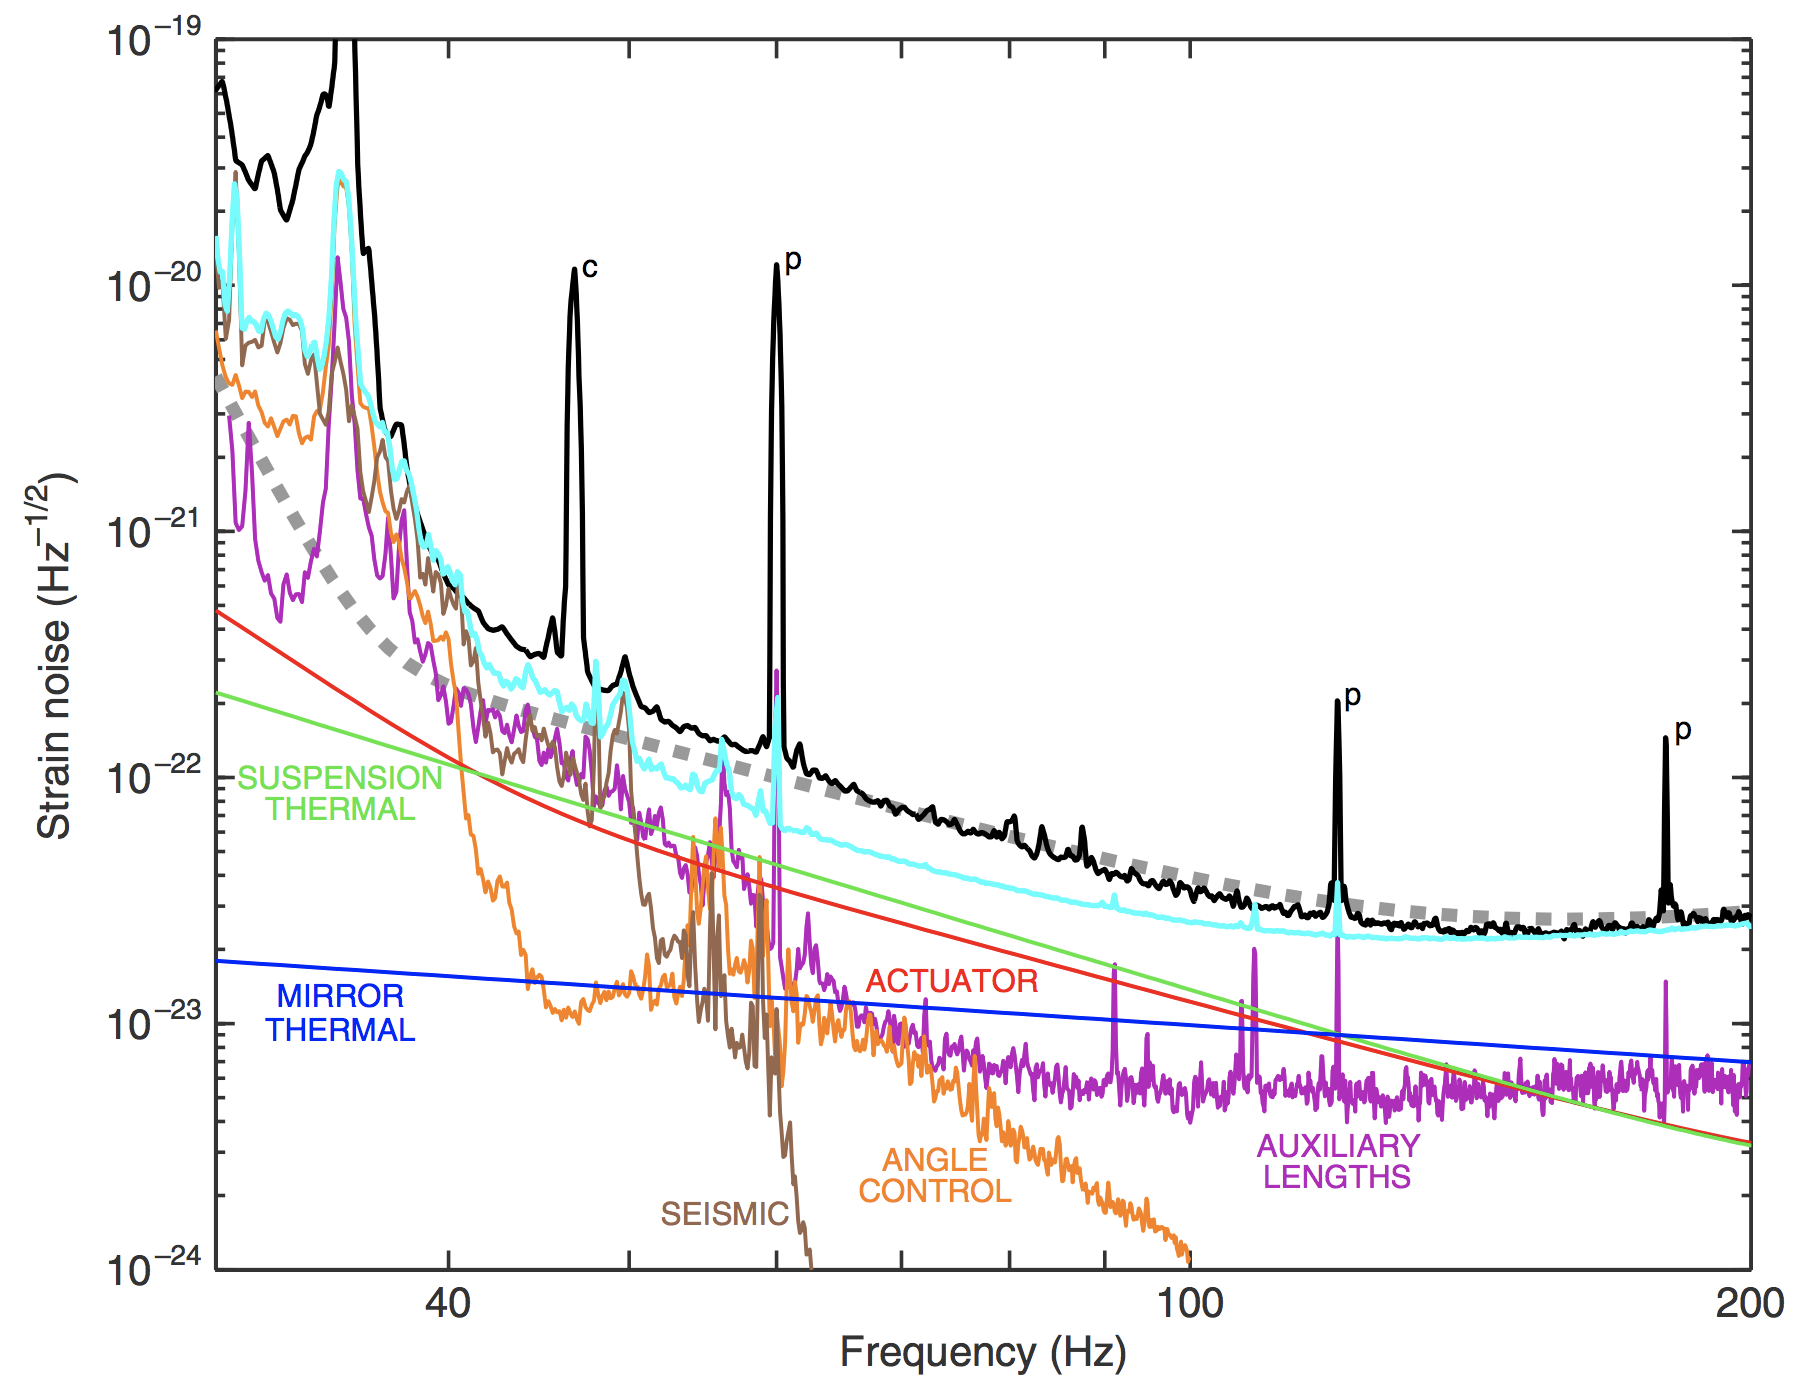
\includegraphics[width=7.5cm]{figures/DisplacementNoise.png}
    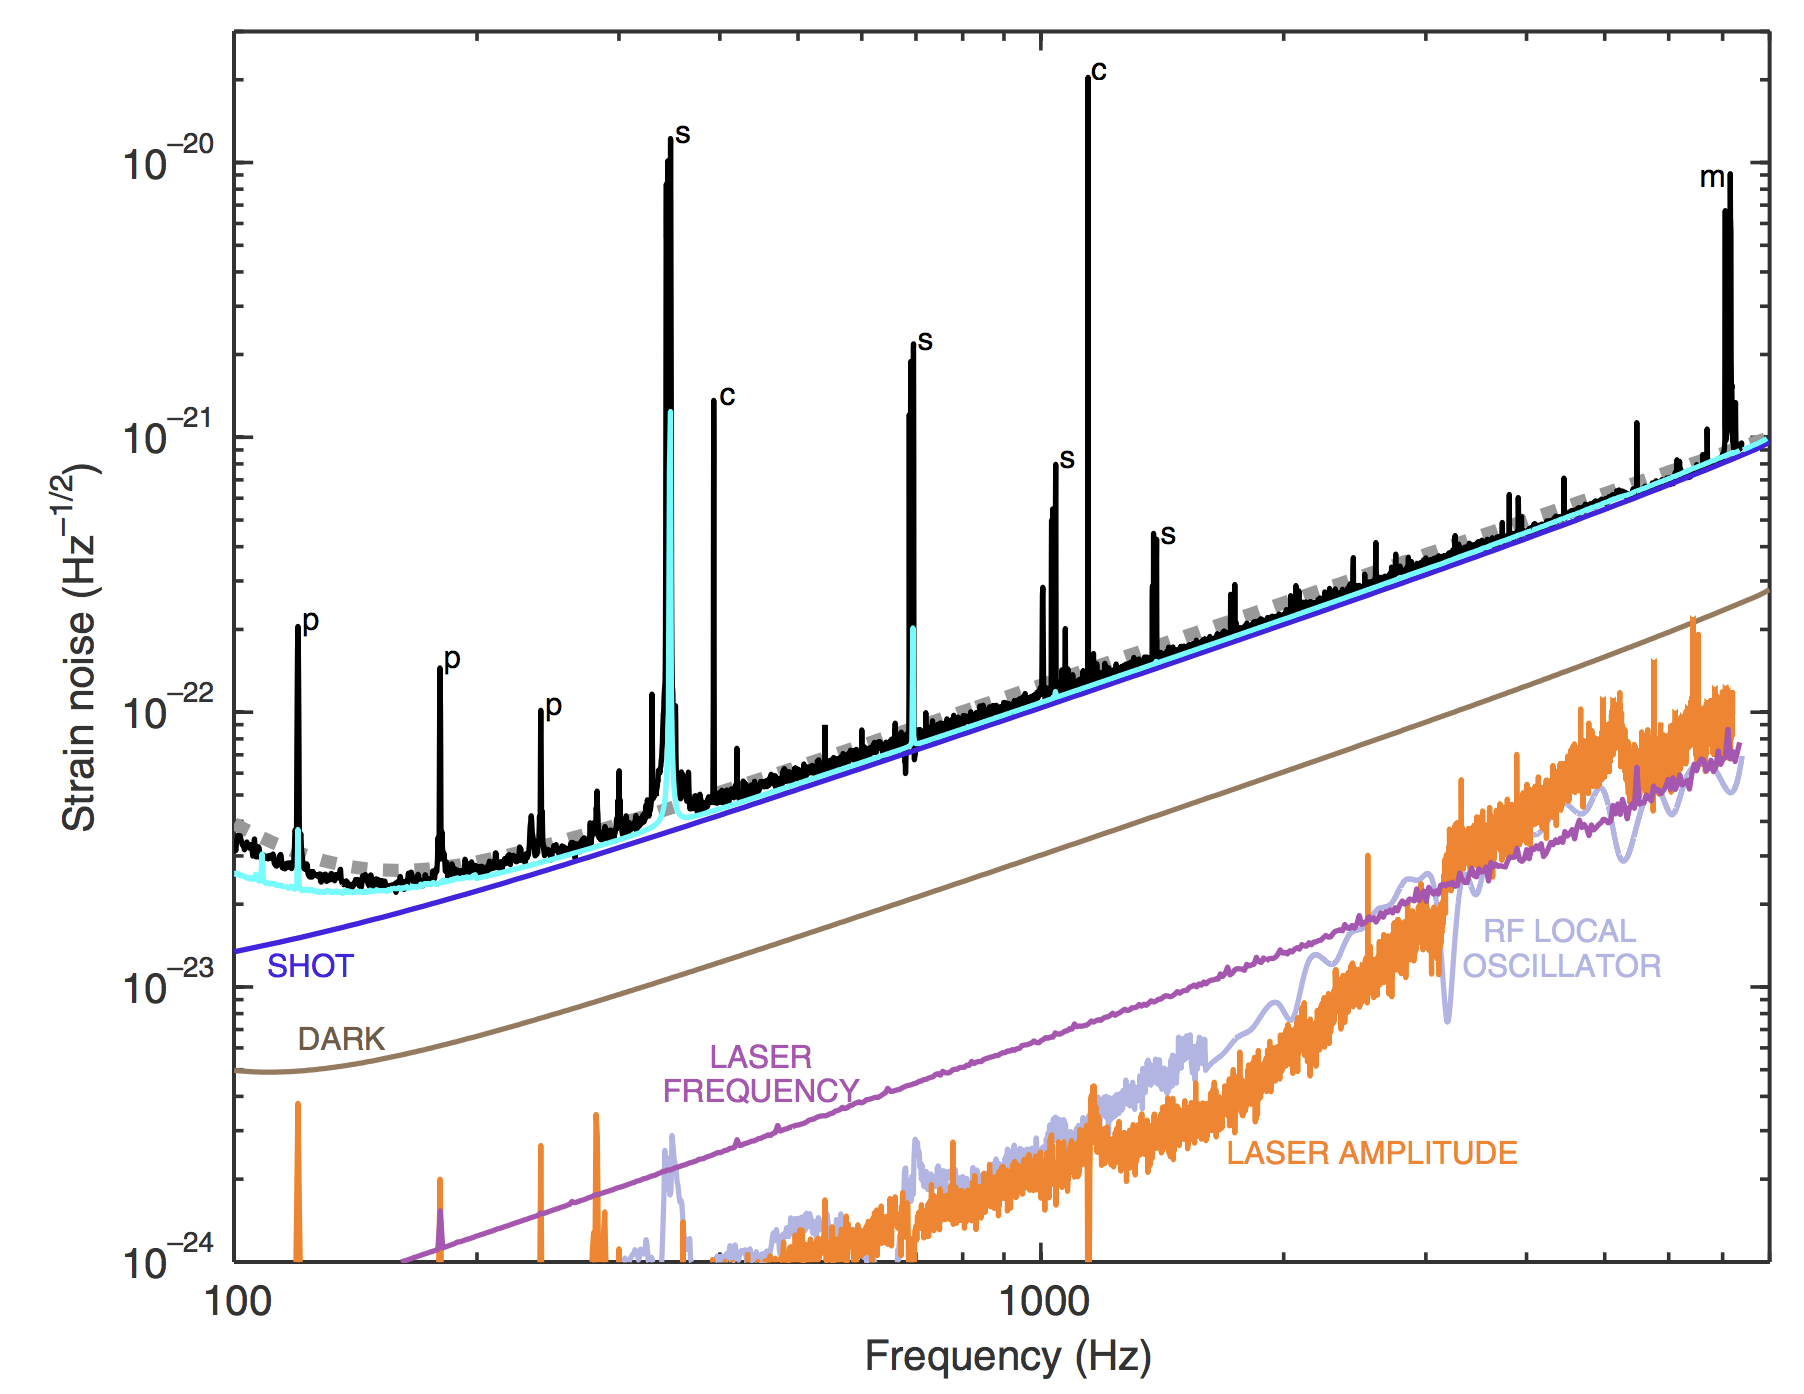
\includegraphics[width=7.5cm]{figures/SensingNoise.png}
    \caption{\footnotesize{Primary known contributors to the H1 detector noise spectrum. The left panel shows the displacement noise components, while the right panel shows sensing noises (note the different frequency scales). In both panels, the black curve is the measured strain noise (same spectrum as in Figure \ref{fig:strainnoise}), the dashed gray curve is the design goal and the cyan curve is the root-square-sum of all known contributors (both sensing and displacement noises). The known noise sources explain the observed noise very well at frequencies above $150\,{\rm Hz}$, and to within a factor of $2$ in the $40-100\,{\rm Hz}$ band. Spectral peaks are identified as follows: c, calibration line; p, power line harmonic; s, suspension wire vibrational mode; m, mirror (test mass) vibrational mode. Figure taken from Abbott (2009).}}
    \label{fig:ligonoise}
\end{figure}

% --------------------------------------------------------------
%               20. 
% --------------------------------------------------------------

\newpage
\subsection{Question 20}

Self-similarity is a useful idealization of many astrophysical systems. Explain what self-similarity means, when it works, and why it is so useful, and provide two examples from any field.

\subsubsection{Short answer}

Answer.

\subsubsection{Additional context}

Additional context.

% --------------------------------------------------------------
%               21. 
% --------------------------------------------------------------

\newpage
\subsection{Question 21}

Explain why diffraction-limited detectors tend to have sidelobes, and how sidelobes can be suppressed in optical and radio observations.

\subsubsection{Short answer}

Answer.

\subsubsection{Additional context}

Additional context.

% --------------------------------------------------------------
%               Resources 
% --------------------------------------------------------------

\newpage
\subsection{Resources}

\begin{itemize}
    \item Astronomical Statistics, Taylor (2004)
    \item Statistical Methods for Astronomical Data Analysis, Chattopadhyay \& Chattopadhyay (2014)
    \item Data Reduction and Error Analysis for the Physical Sciences, Bevington \& Robinson (2003)
    \item Bayesian Logical Data Analysis for the Physical Sciences, Gregory (2005)
    \item Magnetic Fields in Diffuse Media, Lazarian (2015)
    \item Optics, Hecht (2002)
    \item Astronomical Optics, Schroeder (1987)
    \item Handbook of CCD Astronomy, Howell (2006)
    \item Gravitational Waves, Thorne (1994)
    \item Gravitational Bending of Light, Edwards (2007)
    \item Gravitational Lensing, Abdo
    \item Principles of Interferometry, Jackson (2008)
    \item Astrophysics of the Interstellar Medium; Maciel (2013)
    \item Radio Polarimetry as a Probe of Interstellar Magnetism; Newton-McGee (2009)
    \item Synchrotron Radiation; Mobilio et al. (2015)
    \item Cosmic Magnetobremsstrahlung (Synchrotron Radiation); Ginzburg \& Syrovatskii (1965)
    \item The Evolution of Neutrino Astronomy; Bahcall \& Davies (2000)
    \item Observation of Gravitational Waves from a Binary Black Hole Merger; Abbott et al. (2016)
    \item LIGO: the Laser Interferometer Gravitational-Wave Observatory; Abbott et al. (2009)
    \item Self-similar Collapse of Isothermal Spheres and Star Formation; Shu (1977)
    \item Beyond the Diffraction Limit via Optical Amplification; Kellerer \& Ribak (2016)
    \item Log-Normal Distributions Across the Sciences: Keys and Clues; Limpert et al. (2001)
    \item Microlensing; Encyclopedia of Astronomy and Astrophysics (2001)
    \item Interferometry and Synthesis in Radio Astronomy; Thompson et al. (2017)
    \item Essential Radio Astronomy; Condon \& Ransom (2016)
    \item Principles of Interferometry; Jackson
\end{itemize}

\end{document}
